\documentclass{wissdoc}

% Autor: Roland Bless 1996-2009, bless <at> kit.edu
% ----------------------------------------------------------------
% Diplomarbeit - Hauptdokument
% ----------------------------------------------------------------
%%
%% $Id: diplarb.tex 53 2009-12-10 12:23:37Z bless $
%%
% wissdoc Optionen: draft, relaxed, pdf --> siehe wissdoc.cls
% ------------------------------------------------------------------
% Weitere packages: (Dokumentation dazu durch "latex <package>.dtx")
%\usepackage{bibgerm}
%\usepackage[backend=biber]{biblatex} 

\usepackage{csquotes} 
\usepackage{tabularx}
\usepackage{booktabs}
\usepackage{multirow}
%\usepackage{tocbibind}
\usepackage{siunitx}
\usepackage{xcolor}
\usepackage{textcomp}
\usepackage{listings}
\usepackage{newfloat,caption}
\usepackage{subcaption}
\usepackage{footnote}
\usepackage{rotating}
\usepackage{pgfplots}
\usepackage{pgfplotstable}
\usepackage{url}
\usepackage{boxhandler}
\usepackage{tabu}
\usepackage{amssymb}
%\usepackage{subfig}
%\usepackage{subcaption}
%\usepackage{caption}
\usepackage{subcaption}
%\usepackage[plainpages=true]{hyperref}
\usepackage[space]{grffile}
%\usepackage[numbers,sort&compress]{natbib}
\usepackage[backend=bibtex,natbib=true,hyperref=true,doi=false,url=false,style=numeric,sorting=none]{biblatex}

\usepackage{graphicx}

\usepackage{pifont}
\newcommand{\cmark}{\ding{51}}%
\newcommand{\xmark}{\ding{55}}%

%\usepackage{biblatex}
% \usepackage{varioref}
\usepackage{verbatim}
\usepackage{float}    %z.B. \floatstyle{ruled}\restylefloat{figure}
\usepackage[strings]{underscore}
%\usepackage[hidelinks]{hyperref}
% \usepackage{subfigure}
% \usepackage{fancybox} % für schattierte,ovale Boxen etc.
% \usepackage{tabularx} % automatische Spaltenbreite
% \usepackage{supertab} % mehrseitige Tabellen
% \usepackage[svnon,svnfoot]{svnver} % SVN Versionsinformation 
%% ---------------- end of usepackages -------------

%\svnversion{$Id: diplarb.tex 53 2009-12-10 12:23:37Z bless $} % In case that you want to include version information in the footer
%\hyphenation{if...-then...}
%% Informationen für die PDF-Datei

%\usepackage[utf8]{inputenc}

%\DeclareUnicodeCharacter{252C}{\signa}%┬}
%\DeclareUnicodeCharacter{2592}{\signb}%▒}




\pgfplotsset{compat=newest}

\hypersetup{
%%% styling of link inside pdf
	colorlinks,
  citecolor=black,
  filecolor=black,
  linkcolor=black,
  urlcolor=black,
%%%		
 pdfauthor={Sachin Rajgopal},
 pdftitle={Accessible EPUB}
 pdfsubject={Not set},
 pdfkeywords={Not set}
}
\DeclareFloatingEnvironment[fileext=frm,placement={!ht},name=Listing,within=section]{listing}

% Macros, nicht unbedingt notwendig
%%%%%%%%%%%%%%%%%%%%%%%%%%%%%%%%%%%%%%%%%%%%%%%%%%%%%%%%%%
% macros.tex -- einige mehr oder weniger nuetzliche Makros
% Autor: Roland Bless 1998
%%%%%%%%%%%%%%%%%%%%%%%%%%%%%%%%%%%%%%%%%%%%%%%%%%%%%%%%%%
% $Id: macros.tex 33 2007-01-23 09:00:59Z bless $
%%%%%%%%%%%%%%%%%%%%%%%%%%%%%%%%%%%%%%%%%%%%%%%%%%%%%%%%%%


%%%%%%%%%%%%%%%%%%%%%%%
% Kommentare 
%%%%%%%%%%%%%%%%%%%%%%%
\ifnotdraftelse{
\newcommand{\Kommentar}[1]{}
}{\newcommand{\Kommentar}[1]{{\em #1}}}
% Alles innerhalb von \Hide{} oder \ignore{} 
% wird von LaTeX komplett ignoriert (wie ein Kommentar)
\newcommand{\Hide}[1]{}
\let\ignore\Hide

%%%%%%%%%%%%%%%%%%%%%%%%%
% Leere Seite ohne Seitennummer, wird aber gezaehlt
%%%%%%%%%%%%%%%%%%%%%%%%%

\newcommand{\leereseite}{% Leerseite ohne Seitennummer, nächste Seite rechts (wenn 2-seitig)
 \clearpage{\pagestyle{empty}\cleardoublepage}
}
%%%%%%%%%%%%%%%%%%%%%%%%%%
% Flattersatz rechts und Silbentrennung, Leerraum nach rechts maximal 1cm
%%%%%%%%%%%%%%%%%%%%%%%%%%
\makeatletter
\newcommand{\myraggedright}{%
 \let\\\@centercr\@rightskip 0pt plus 1cm
 \rightskip\@rightskip
  \leftskip\z@skip
  \parindent\z@
  \spaceskip=.3333em
  \xspaceskip=.5em}
\makeatother

\makeatletter
\newcommand{\mynewline}{%
 \@centercr\@rightskip 0pt plus 1cm
}
\makeatother


%%%%%%%%%%%%%%%%%%%%%%%%%%
% Für Index
%%%%%%%%%%%%%%%%%%%%%%%%%%
\makeatletter
\def\mydotfill{\leavevmode\xleaders\hb@xt@ .44em{\hss.\hss}\hfill\kern\z@}
\makeatother
\def\bold#1{{\bfseries #1}}
\newbox\dbox \setbox\dbox=\hbox to .4em{\hss.\hss} % dot box for leaders
\newskip\rrskipb \rrskipb=.5em plus3em % ragged right space before break
\newskip\rrskipa \rrskipa=-.17em plus -3em minus.11em % ditto, after
\newskip\rlskipa \rlskipa=0pt plus3em % ragged left space after break
\newskip\rlskipb \rlskipb=.33em plus-3em minus.11em % ragged left before break
\newskip\lskip \lskip=3.3\wd\dbox plus1fil minus.3\wd\dbox % for leaders
\newskip \lskipa \lskipa=-2.67em plus -3em minus.11em %after leaders
\mathchardef\rlpen=1000 \mathchardef\leadpen=600
\def\rrspace{\nobreak\hskip\rrskipb\penalty0\hskip\rrskipa}
\def\rlspace{\penalty\rlpen\hskip\rlskipb\vadjust{}\nobreak\hskip\rlskipa}
\let\indexbreak\rlspace
\def\raggedurl{\penalty10000 \hskip.5em plus15em \penalty0 \hskip-.17em plus-15em minus.11em}
\def\raggeditems{\nobreak\hskip\rrskipb \penalty\leadpen \hskip\rrskipa %
\vadjust{}\nobreak\leaders\copy\dbox\hskip\lskip %
\kern3em \penalty\leadpen \hskip\lskipa %
\vadjust{}\nobreak\hskip\rlskipa}
\renewcommand*\see[2]{\rlspace\emph{\seename}~#1} % from makeidx.sty

%%%%%%%%%%%%%%%%%%%%%%%%%%
% Neue Seite rechts, leere linke Seite ohne Headings
%%%%%%%%%%%%%%%%%%%%%%%%%%
\newcommand{\xcleardoublepage}
{{\pagestyle{empty}\cleardoublepage}}

%%%%%%%%%%%%%%%%%%%%%%%%%%
% Tabellenspaltentypen (benoetigt colortbl)
%%%%%%%%%%%%%%%%%%%%%%%%%%
\newcommand{\PBS}[1]{\let\temp=\\#1\let\\=\temp}
\newcolumntype{y}{>{\PBS{\raggedright\hspace{0pt}}}p{1.35cm}}
\newcolumntype{z}{>{\PBS{\raggedright\hspace{0pt}}}p{2.5cm}}
\newcolumntype{q}{>{\PBS{\raggedright\hspace{0pt}}}p{6.5cm}}
\newcolumntype{g}{>{\columncolor[gray]{0.8}}c} % Grau
\newcolumntype{G}{>{\columncolor[gray]{0.9}}c} % helleres Grau

%%%%%%%%%%%%%%%%%%%%%%%%%%
% Anführungszeichen oben und unten
%%%%%%%%%%%%%%%%%%%%%%%%%%
\newcommand{\anf}[1]{"`{#1}"'}

%%%%%%%%%%%%%%%%%%%%%%%%%%
% Tiefstellen von Text
%%%%%%%%%%%%%%%%%%%%%%%%%%
% S\tl{0} setzt die 0 unter das S (ohne Mathemodus!)
% zum Hochstellen gibt es uebrigens \textsuperscript
\makeatletter
\DeclareRobustCommand*\textlowerscript[1]{%
  \@textlowerscript{\selectfont#1}}
\def\@textlowerscript#1{%
  {\m@th\ensuremath{_{\mbox{\fontsize\sf@size\z@#1}}}}}
\let\tl\textlowerscript
\let\ts\textsuperscript
\makeatother

%%%%%%%%%%%%%%%%%%%%%%%%%%
% Gauß-Klammern
%%%%%%%%%%%%%%%%%%%%%%%%%%
\newcommand{\ceil}[1]{\lceil{#1}\rceil}
\newcommand{\floor}[1]{\lfloor{#1}\rfloor}

%%%%%%%%%%%%%%%%%%%%%%%%%%
% Average Operator (analog zu min, max)
%%%%%%%%%%%%%%%%%%%%%%%%%%
\def\avg{\mathop{\mathgroup\symoperators avg}}

%%%%%%%%%%%%%%%%%%%%%%%%%%
% Wortabkürzungen
%%%%%%%%%%%%%%%%%%%%%%%%%%
\def\zB{z.\,B.\ }
\def\dh{d.\,h.\ }
\def\ua{u.\,a.\ }
\def\su{s.\,u.\ }
\newcommand{\bzw}{bzw.\ }

%%%%%%%%%%%%%%%%%%%%%%%%%%%%%%%%%%%
% Einbinden von Graphiken
%%%%%%%%%%%%%%%%%%%%%%%%%%%%%%%%%%%
% global scaling factor
\def\gsf{0.9}
%% Graphik, 
%% 3 Argumente: Datei, Label, Unterschrift
\newcommand{\Abbildung}[3]{%
\begin{figure}[tbh] %
\centerline{\scalebox{\gsf}{\includegraphics*{#1}}} %
\caption{#3} %
\label{#2} %
\end{figure} %
}
\let\Abb\Abbildung
%% Abbps
%% Graphik, skaliert, Angabe der Position
%% 5 Argumente: Position, Breite (0 bis 1.0), Datei, Label, Unterschrift
\newcommand{\Abbildungps}[5]{%
\begin{figure}[#1]%
\begin{center}
\scalebox{\gsf}{\includegraphics*[width=#2\textwidth]{#3}}%
\caption{#5}%
\label{#4}%
\end{center}
\end{figure}%
}
\let\Abbps\Abbildungps
%% Graphik, Angabe der Position, frei wählbares Argument für includegraphics
%% 5 Argumente: Position, Optionen, Datei, Label, Unterschrift
\newcommand{\Abbildungpf}[5]{%
\begin{figure}[#1]%
\begin{center}
\scalebox{\gsf}{\includegraphics*[#2]{#3}}%
\caption{#5}%
\label{#4}%
\end{center}
\end{figure}%
}
\let\Abbpf\Abbildungpf

%%
% Anmerkung: \resizebox{x}{y}{box} skaliert die box auf Breite x und Höhe y,
%            ist x oder y ein !, dann wird das usprüngliche 
%            Seitenverhältnis beibehalten.
%            \rescalebox funktioniert ähnlich, nur das dort ein Faktor
%            statt einer Dimension angegeben wird.
%%
% \Abbps{Position}{Breite in Bruchteilen der Textbreite}{Dateiname}{Label}{Bildunterschrift}
%

\newcommand{\refAbb}[1]{%
s.~Abbildung \ref{#1}}

%%%%%%%%%%%%%%%%%%%%
%% end of macros.tex
%%%%%%%%%%%%%%%%%%%%

\renewcommand{\familydefault}{\sfdefault}
% Print URLs not in Typewriter Font
\def\UrlFont{\rm}

\newcommand{\specialcell}[2][c]{%
  \begin{tabular}[#1]{@{}c@{}}#2\end{tabular}}

\newcommand\todo[1]{\textcolor{red}{TODO: #1}}

\newcommand\hlcode[1]{\textcolor{red}{#1}}

\newcommand\citeable[1]{\textcolor{green}{\hl{citeable: #1}}}

\newcolumntype{$}{>{\global\let\currentrowstyle\relax}}
\newcolumntype{^}{>{\currentrowstyle}}
\newcommand{\rowstyle}[1]{\gdef\currentrowstyle{#1}%
  #1\ignorespaces
}

\newif\ifcomment
%\commenttrue %# Show comments


\newcommand{\blankpage}{% Leerseite ohne Seitennummer, nächste Seite rechts
 \clearpage{\pagestyle{empty}\cleardoublepage}
}

%% Einstellungen für das gesamte Dokument

% Trennhilfen
% Wichtig! 
% Im german-paket sind zusätzlich folgende Trennhinweise enthalten:
% "- = zusätzliche Trennstelle
% "| = Vermeidung von Ligaturen und mögliche Trennung (bsp: Schaf"|fell)
% "~ = Bindestrich an dem keine Trennung erlaubt ist (bsp: bergauf und "~ab)
% "= = Bindestrich bei dem Worte vor und dahinter getrennt werden dürfen
% "" = Trennstelle ohne Erzeugung eines Trennstrichs (bsp: und/""oder)

% Trennhinweise fuer Woerter hier beschreiben
\hyphenation{
% Pro-to-koll-in-stan-zen
% Ma-na-ge-ment  Netz-werk-ele-men-ten
% Netz-werk Netz-werk-re-ser-vie-rung
% Netz-werk-adap-ter Fein-ju-stier-ung
% Da-ten-strom-spe-zi-fi-ka-tion Pa-ket-rumpf
% Kon-troll-in-stanz
}
\lstset{
    frame=single,
    breaklines=true,
		basicstyle=\scriptsize,
	 escapeinside={\%*}{*)},
    %postbreak=\raisebox{0ex}[0ex][0ex]{\ensuremath{\color{red}\hookrightarrow\space}}
}

% Index-Datei öffnen
\ifnotdraft{\makeindex}
%%%%%%%%%%%%%% includeonly %%%%%%%%%%%%%%%%%%%
% Es werden nur die Teile eingebunden, die hier 
% aufgefuehrt sind!
\includeonly{%
titlepage,%
statement,% Ist in KA Pflicht für Diplomarbeiten
introduction,% Motivation, Zielsetzung, Gliederung
background,% Grundlagen 
%analysis,   % Problembeschreibung (Detail) und Related Work
%design,   % Beschreibung der Problemlösung (Konzepte, allg. Architektur, ...)
%implementation,  % Beschreibung der Umsetzung/Implementierung
%evaluation,      % Nachweis und Auswertung
epubDocumentStandard,
evaluationEpubStandard,
editor,
evaluationEditor,
futurework,% Future Work
summary  % Zusammenfassung der Ergebnisse 
}

\bibliography{Literature, Websites}
\bibliography{Accessible_EPUB}

\usepgfplotslibrary{groupplots}
\usetikzlibrary{pgfplots.groupplots}
%\addbibresource{diplarb.bib}

%%%%%%%%%%%%%%%%%%%%%%%%%%%%%%%%%%%%%%%%%%%%%%
\begin{document}

\frontmatter
\pagenumbering{roman}
\ifnotdraft{
 %% Titelseite
%% Vorlage $Id: titelseite.tex 54 2009-12-10 12:23:58Z bless $

\def\usesf{}
\let\usesf\sffamily % diese Zeile auskommentieren für normalen TeX Font

\newsavebox{\Erstgutachter}
\savebox{\Erstgutachter}{\usesf Prof.~Dr.~Rainer Stiefelhagen}
\newsavebox{\Zweitgutachter}
\savebox{\Zweitgutachter}{\usesf \todo{Eintragen}}

\begin{titlepage}
\setlength{\unitlength}{1pt}

\begin{picture}(0,0)(85,770)

\includegraphics[width=\paperwidth]{logos/KIT_Deckblatt}
\end{picture}

\vspace*{-45pt}\hspace*{400pt}
\includegraphics[width=.1\paperwidth]{logos/SZS.png}

\thispagestyle{empty}

%\begin{titlepage}
%%\let\footnotesize\small \let\footnoterule\relax
\begin{center}
\hbox{}
\vfill
{\usesf
{\huge\bfseries Accessible EPUB
 \par}
\vskip 1.8cm
Bachelor Thesis\\
by\\[2mm]
\vskip 1cm

{\large\bfseries Sachin Rajgopal\\}
\vskip 1.2cm
Study Centre for the Visually Impaired Students (SZS)\\
Department of Informatics\\
%Universität Karlsruhe (TH)\\[2ex]
\vskip 3cm
\begin{tabular}{p{5.5cm}l}
First Reviewer: & \usebox{\Erstgutachter} \\
Second Reviewer: & \usebox{\Zweitgutachter} \\
Supervisor: & Dr. Thorsten Schwarz \\
\end{tabular}
\vskip 3cm
Project Period:\qquad 01/12/2017 -- XX/XX/20XX
}
\end{center}
\vfill
\end{titlepage}
%% Titelseite Ende


%%% Local Variables: 
%%% mode: latex
%%% TeX-master: "diplarb"
%%% End: 

 \blankpage % Leerseite auf Titelrückseite
 %
 % Die folgende Erklärung ist für Diplomarbeiten Pflicht
 % (siehe Prüfungsordnung), für Studienarbeiten nicht notwendig
 \thispagestyle{empty}
\vspace*{42\baselineskip}
\hbox to \textwidth{\hrulefill}
\par
Ich versichere wahrheitsgemäß, die Arbeit selbstständig angefertigt, alle benutzten Hilfsmittel vollständig und genau angegeben und alles kenntlich gemacht zu haben, was aus Arbeiten anderer unverändert oder mit Abänderungen entnommen wurde.

Karlsruhe, den \todo{date}

\cleardoublepage

\vspace*{1em}
\begin{center}
	\textbf{Zusammenfassung}
\end{center}
\par
\todo{Zusammenfassung (Deutsch)}
\cleardoublepage
\vspace*{1em}
\begin{center}
	\textbf{Abstract}
\end{center}
\par
\todo{Zusammenfassung (Englisch)}

\cleardoublepage


 \blankpage % Leerseite auf Erklärungsrückseite
}
%
%% *************** Hier geht's ab ****************
%% ++++++++++++++++++++++++++++++++++++++++++
%% Verzeichnisse
%% ++++++++++++++++++++++++++++++++++++++++++
\ifnotdraft{
{\parskip 0pt\tableofcontents} % toc bitte einzeilig
%\pagenumbering{roman}
%\cleardoublepage
%\addcontentsline{toc}{chapter}{\listfigurename}
%\listoffigures
%
%\cleardoublepage
%\addcontentsline{toc}{chapter}{\listtablename}
%\listoftables
%\addcontensline{toc}{section}{List of Tables}
%\pagenumbering{roman}
%\listoffigures
%\addcontensline{toc}{section}{List of Figures}
%\blankpage
%\listoffigures
%\blankpage
%\listoftables
%\blankpage
}
\cleardoublepage
%\blankpage

%% ++++++++++++++++++++++++++++++++++++++++++
%% Hauptteil
%% ++++++++++++++++++++++++++++++++++++++++++
\graphicspath{{images/}}

\mainmatter
%\null
%\newpage
\pagenumbering{arabic}
%% Einleitung.tex
%% $Id: einleitung.tex 28 2007-01-18 16:31:32Z bless $
%%

\chapter{Introduction}
\label{ch:Introduction}
%% ==============================
% CLEARLY SHOW CONTRIBUTIONS AND LINK THEM TO SECTIONS
  % Einleitung
%% grundlagen.tex
%% $Id: grundlagen.tex 28 2007-01-18 16:31:32Z bless $
%%

\chapter{Related Work}
\label{ch:RelatedWork}

A project which also uses HTML/XHTML to make documents accessible is discussed in a paper \cite{markdownSyntax} by Voegler et al.. HTML is chosen as a book format, because it is operating system independent, accessible to screen readers and the content can be adapted visually to a person's wishes.  However, the work is generally not done by the original document author. Instead university/service staff or students transcribe it to accessible versions. They have to request the content from authors and get permission. 
Coding with HTML creates problems like linking errors, invalid HTML-code, etc., so Voegler et al. recommend using Markdown \cite{Markdown}, which is easier to write than HTML. It can then be converted to a variety of formats using pandoc \cite{Pandoc}, which also converts \LaTeX code to MathML.
While reducing the number of mistakes compared to HTML, Markdown still requires programming and only people with sufficient knowledge of it will be able to use it effectively. Students doing the transcription will be more knowledgeable in coding than teachers in schools for the blind. 

If EPUB is compared to HTML as book format, it is of course very similar as EPUB uses HTML/XHTML. HTML as a book format can be described as a simplified version of EPUB only without the packaging such as the package document, in essence only having the OEBPS folder. However, images have to be added manually to the folders, and CSS files have to be created. These are extra steps that might result in frequent mistakes. Furthermore, Pandoc is command line based and is therefore more difficult to use than programs with a graphical user interface (GUI). It also has to be run separately after coding in Markdown, instead of being integrated in the creation process. Nevertheless, this paper shows that HTML, if created properly, is suitable to the needs of blind and visually impaired students.

Another approach is offered by Leporini et al. in their project Book4All \cite{book4all}. It originally allowed PDFs to be exported to XHTML or DAISY, later EPUB 3 was added as an option. It reads the PDF with the PDF Viewer to gather information about fonts and recognize if the document is in a multi-column layout. Then Book4All has to take this information and extracts the text and semantic information. This includes keeping the format of the PDF, such as recognizing headings, images and tables being properly tagged. The user has the option of correcting tagging mistakes. It then has to be exported to its final format. 

\begin{figure}[H]
	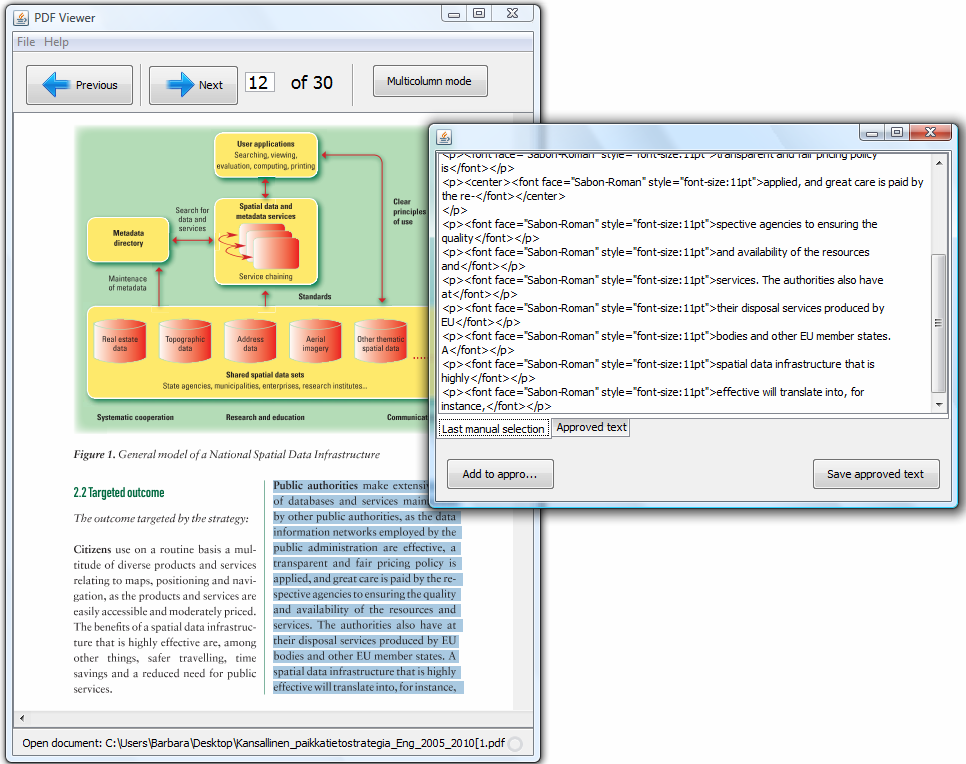
\includegraphics[width=\linewidth]{figures/book4all1.png}
	\caption{A view of the ad-hoc PDF Viewer extracting text from a multi-column layout document \protect\cite{book4all}}
	\label{fig:book4all1}
\end{figure}

Book4All attempts to semi-automate the conversion process as far as possible, but still offers the option of post processing the resulting markup as shown in figure~\ref{fig:book4all1}. While this is optional, important parts like alternative text for images can only be added like this. The markup is in Intermediate Book Format (IBF), which is based on XML. Without basic knowledge of XML, post-processing becomes much more difficult. 

\begin{figure}[H]
	\centering
	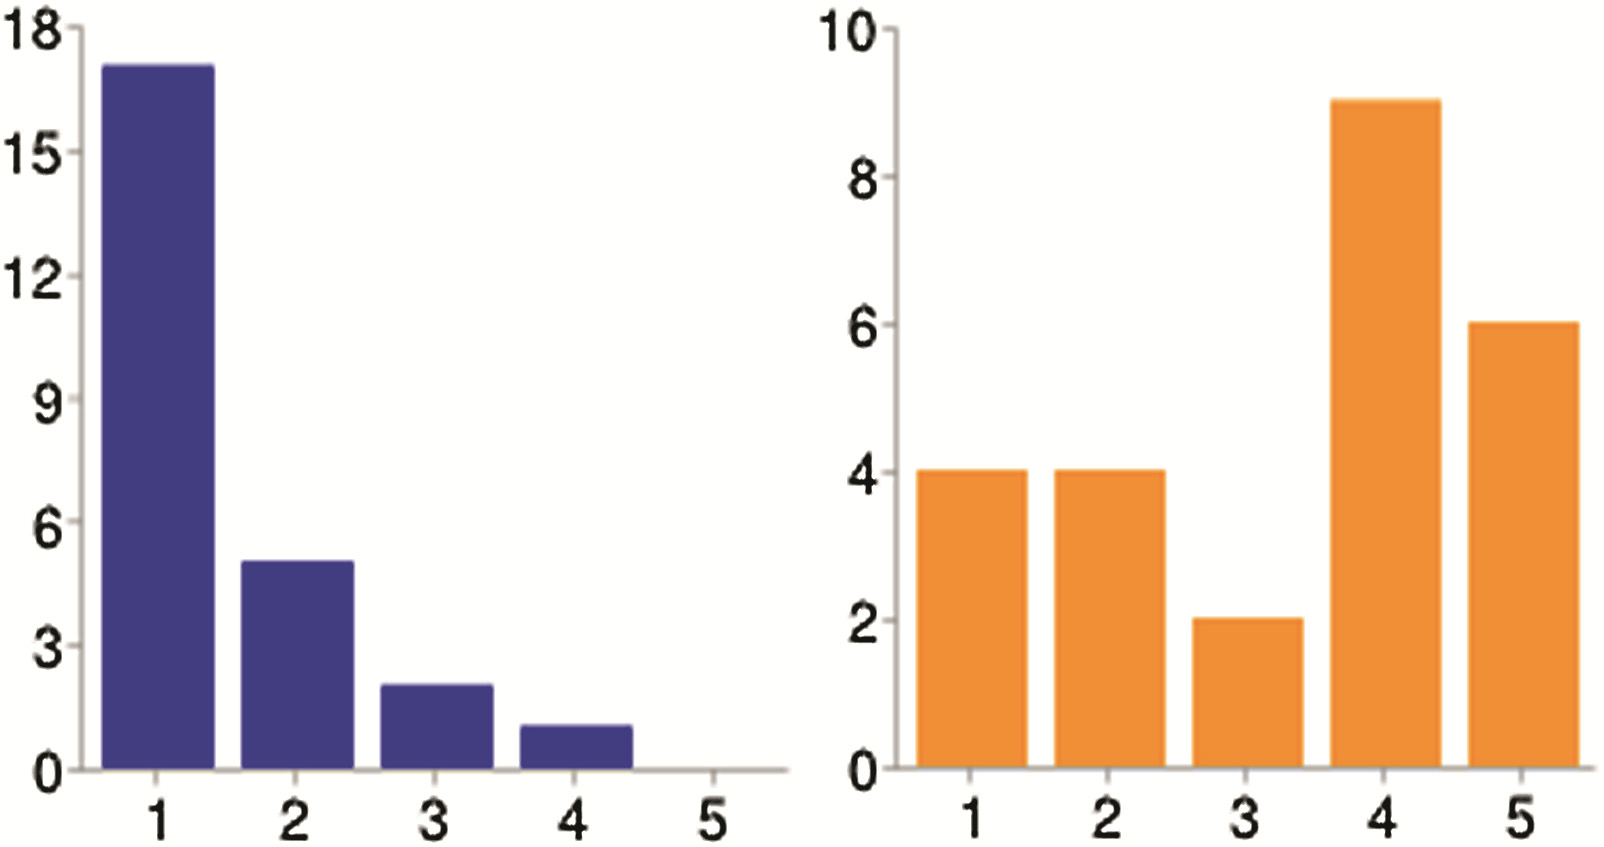
\includegraphics[width=\linewidth*4/5]{figures/easeOfContentAccess.png}
	\caption{Difficulty degree to access the content for the EPUB (blue, left) and PDF (orange, right), respectively (1-not difficult
		to 5-very difficult) \protect\cite{enrichEPUB}} 
	\label{fig:enrichEpub1}
\end{figure}

Bartalesi and Leporini \cite{enrichEPUB} also carried out an online survey in a follow-up work and asked 25 users to rate "enriched" EPUBs created in Book4All in comparison to the original PDF format regarding accessibility and usability. $50\%$ of respondents preferred EPUB over other e-book formats, while $13\%$ said EPUB was equivalent.
The sample group also felt that it was easier to access content in EPUBs and use the table of contents than in PDFs.
Furthermore, $80\%$ of blind users were unable to read images in PDFs correctly with their screen reader, while the corresponding value for EPUBs was less than $50\%$. $64\%$ of users found the EPUB's document structure easy to understand. Users also reported that it is much easier to access content in the EPUB than in a PDF, as shown in figure~\ref{fig:enrichEpub1}.  The results show that EPUB is suitable format for blind people, if the EPUB contains proper tagging. 
Those works motivate us to develop a new universal approach.

  % Grundlagen
\chapter{EPUB Document Standard}
\label{ch:EPUB Document Standard}

\section{Requirements}

One requirement of the new standard is that incorporates a way to switch between three versions, them being:

\begin{itemize}
	\item Blind
	\item Visually impaired
	\item Normal/sighted 
\end{itemize}

Switching between three versions should be simple and visible. It should not be hidden behind menus and settings and must be part of the document itself. A document of the standard must conform to EPUB 3 and not rely on external programs to switch between the versions.

The specifications of each version will be compared with each important component of a document.


\subsection{Switching between versions}

Initially the intent was to find one new standard so that EPUB documents can be accessible. Unfortunately, creating a single standard was not possible due to not all EPUB readers supporting all EPUB 3 features.

\subsubsection{JavaScript}
JavaScript is used to make websites interactive, so it was the logical option to dynamically change the versions. The coding was also quite simple and only involved replacing a single line in the CSS file with programming. This was easy to do in JavaScript, and testing the individual XHTML files in the EPUB showed that it was successful. 

Shown in \ref{fig:jsStyleCss} is style.css which just imports the rules of a CSS file. The methods \lstinline|selectVisible()|, \lstinline|selectImpaired()| and \lstinline|selectBlind()| in script.js all function in the same way. To remember the version chosen, local and session storage is used. First they check if local storage is available. If it is then the method attempts to get the item \lstinline|accessibleEPUBcurrentCSS|. If it does not exist, then it is created. This item is then set with the same import line in figure \ref{fig:jsStyleCss}, only with different CSS file name for each version. If local storage is not available the same process is repeated with session storage. Local storage is preferable to session storage as changes are kept even after the program has been exited. This is not the case with session storage so the user has to set version again at the start of the program. Afterwards the method \lstinline|loadCSS()| is called which deletes the CSS rule of a XHTML file and adds the rule set by the earlier methods.

The content of the XHTML file responsible for the switching mechanism, VersionChanger.xhtml, is shown in figure \ref{fig:js_switch}. It is important that both style.css and script.js are referred to, or the switchi mechanism would be unsuccessful. In the body of the XHTML document, the method \lstinline{storageCSS()} is called whenever the XHTML file is loaded, so whenever the XHTML are switched back to it from another. This method checks if local and then session storage are available. If either one is avaiable then it sets the item in the storage and calls \lstinline{loadCSS()}.

\begin{figure}
	
	\begin{lstlisting}
	@import url("../Styles/visible.css");
	\end{lstlisting}
	\caption{Contents of style.css}
	\label{fig:jsStyleCss}
\end{figure}

\begin{figure}
	
	\begin{lstlisting}
	<head>
	<title></title>
	<link rel="stylesheet" href="../Styles/style.css"/>
	<script src="../Misc/script.js"></script>
	</head>
	
	<body epub:type="frontmatter" onload="storageCSS();">
	<a id="a1" href="#a1" onclick="selectVisible();">Normal</a>
	<a id="a2" href="#a2" onclick="selectImpaired();">Visually impaired</a>
	<a id="a3" href="#a3" onclick="selectBlind();">Blind</a>
	</body>
	\end{lstlisting}
	\caption{The links in the JavaScript version}
	\label{fig:js_switch}
\end{figure}

There are some issues with JavaScript version changer. If the software or hardware reader does not support temporary storage, the EPUB is always displayed in its default appearance. Due to this, switching with JavaScript is not a reliable option. As mentioned in chapter \ref{ch:Introduction}, JavaScript does not have to be supported by all EPUB readers. Nevertheless, the JavaScript implementation supports multiple XHTML files, because temporary storage is supported. For the same reason table of contents are also supported, as they are normally displayed in a separate file, named \lstinline|nav.xhtml|. 

\subsubsection{CSS}
The second method does not use JavaScript and uses some advanced features of CSS, introduced in CSS 3. This mainly refers to CSS selectors. Selectors allow HTML documents to have limited interactive capabilities, such as changing the appearance of a clicked element.\cite{cssSelectors}\footnote{https://www.w3schools.com/cssref/css\_selectors.asp} 

Before showing how the selectors work, the format of the content file should be discussed. It is shown in figure~\ref{fig:css_switch}. Unlike the JavaScript version, the links are in the same XHTML file and are shown at the beginning of the EPUB file. In the JavaScript version, the links are on a separate page.


\begin{figure}
	
	\begin{lstlisting}
	<body>
	<a class="versionChanger" id="a1" href="#visible">Normal</a>
	<a class="versionChanger" id="a2" href="#impaired">Visually impaired</a>
	<a class="versionChanger" id="a3" href="#blind">Blind</a>
	
	<div style="padding:none" id="impaired" class="impaired">
	...
	</div>
	<div id="blind" class="blind">
	...
	</div>
	<div id="visible" class="visible">
	...
	</div>
	</body>
	\end{lstlisting}
	\caption{The links and divs in the CSS version}
	\label{fig:css_switch}
\end{figure}

The code shown in figure~\ref{fig:css_selector} is responsible for the switching mechanism. At first only the visible version can be seen and the other two are hidden. The versions appear with the \lstinline|:target| selector, which affects the appearance of the element if it was a target of a link(\lstinline|<a> element|). If another link was clicked, then the current version becomes hidden again. However, the visible version would not become hidden, and this was a major problem. CSS selectors have limited capabilities compared to JavaScript, because they were intended to complement and not replace each other. After a bit of experimentation with various CSS selectors, the \lstinline|~| selector delivered the desired results. \lstinline|~| allows every element on the right hand side to be selected if it preceded by a left hand side element. So in the case of \lstinline|.impaired:target ~ .visible|, once the impaired link has been clicked, the visible sections becomes hidden.

\begin{figure}
	
	\begin{lstlisting}
	.visible {
	display:inline; 
	}
	
	.impaired:target ~ .visible {
	display:none; 
	}
	
	.blind:target ~ .visible {
	display:none; 
	}
	
	.impaired {
	display:none; 
	}
	
	.blind {
	display:none; 
	}
	
	.impaired:target{
	display:inline; 
	}
	
	.blind:target{
	display:inline; 
	}
	\end{lstlisting}
	\caption{The CSS selectors responsible for the dynamic version switching}
	\label{fig:css_selector}
\end{figure}

\subsection{Text}

The blind version does not have to have any special requirements for text, and its appearance will be identical to the normal version. The text size could be made much smaller, but leaving it at a standard size will allow other people to also read the text, such as for proofreading of the blind version.

The visually impaired version needs to use sans-serif fonts, as seen in figure \ref{fig:sansSerif}, instead of serif fonts, as it easier to read and identify individual characters.\cite{pdfBarrierefrei} Furthermore, the font should be larger than the normal version. 

\begin{figure}
	
	\begin{center}
		
\includegraphics[width=\linewidth/2]{figures/sansSerif.jpg}
	\end{center}

	
	\caption{Comparison of serif(left) and sans serif(right) fonts
		\\Source: https://cdncms.fonts.net/images/6bff0c2cdbbcca14/A.SerifSansPrint.jpg}
	\label{fig:sansSerif}
\end{figure}

The font of the normal version can be any font, but for this standard a serif font was chosen. Most importantly, the text should not go beyond the edge of the screen so that horizontal scrolling is not required. All normal text in the document will be between \lstinline|<p>| and \lstinline|</p>| tags. A comparison of the visually impaired and normal version can be seen in figures \ref{fig:viText} and \ref{fig:nText}. 

\begin{figure}
	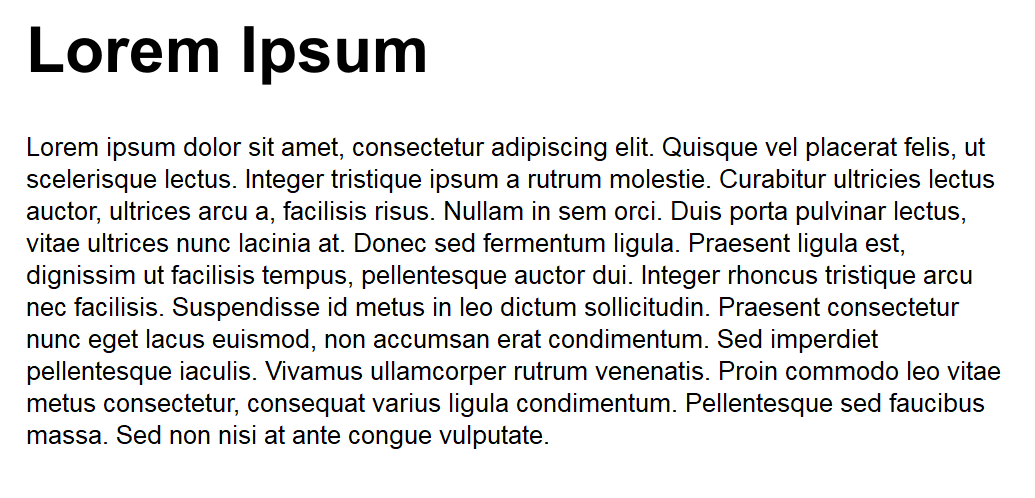
\includegraphics[width=\linewidth]{figures/VItext.png}	
	\caption{Text of the visually impaired version}
	\label{fig:viText}
\end{figure}

\begin{figure}
	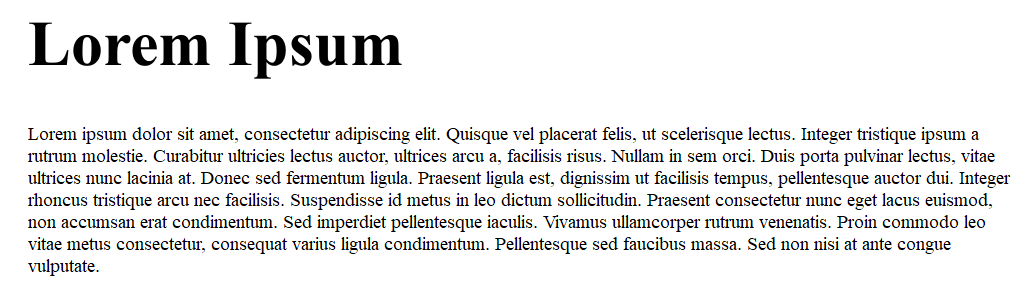
\includegraphics[width=\linewidth]{figures/Ntext.png}	
	\caption{Text of the normal version}
	\label{fig:nText}
\end{figure}

\subsection{Images}

All images need to have alternative text to describe them and preferably have a title given to them. This will help blind users as the screen reader will read out both of them. Usually the alternative text will be set as a property and the screen reader will have to identify the image. However, there was an issue. In some programs the screen reader does not read out the alternative text, so a different way had to be found to display it. The image will be part of a figure element of HTML5, shown in figure~\ref{fig:image_code}. A figure can also contain a caption, which will be identified by the screen reader as such, seen in  figure~\ref{fig:image_viimp} Furthermore, the alternative text will be inserted as a paragraph with the \lstinline|<p>| element. It will remain invisible in normal and visually impaired mode, but will appear as normal text in blind mode. The text should be surrounded by specific tags, like <Image> or <Graph> shown in figure~\ref{fig:image_blind}. It also has the CSS class "transparent", which only appears in blind mode.

Images in visually impaired and normal mode will be displayed normally, but the image, caption and figure will all have a maximum length of 100\% of the screen size.

\begin{figure}[H]
	\centering
	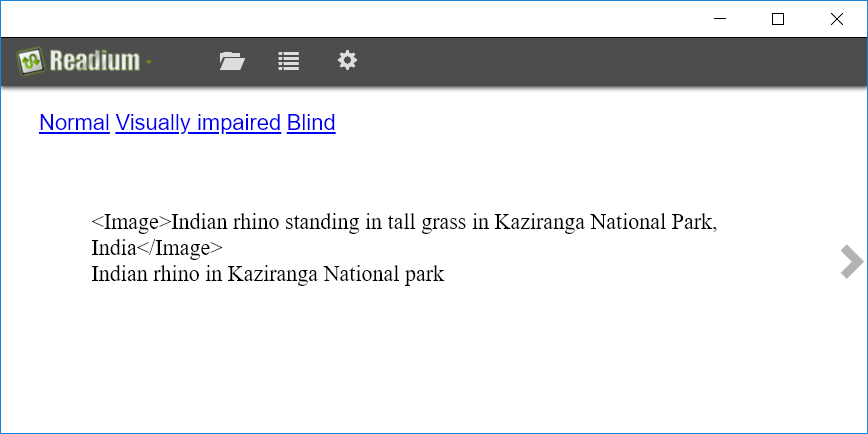
\includegraphics[width=\linewidth]{figures/ImageBl.PNG}
	\caption{Image in 'Blind' mode}
	\label{fig:image_blind}
\end{figure}

\begin{figure}[H]
	\centering
	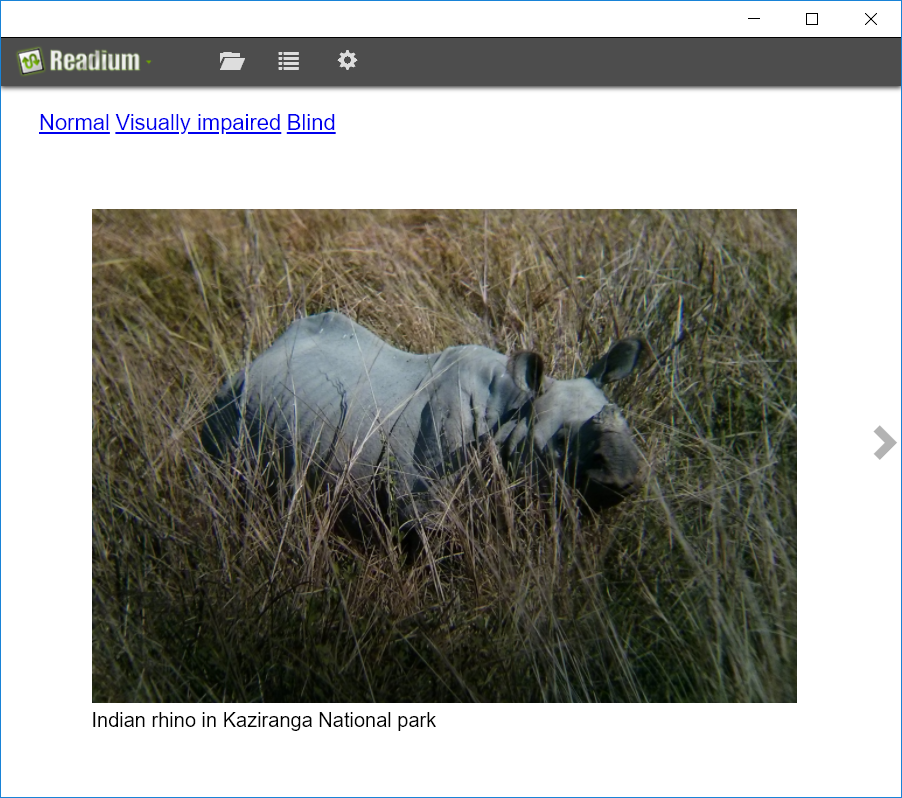
\includegraphics[width=\linewidth]{figures/ImageVi.PNG}
	\caption{Image in 'Visual impairment' mode}
	\label{fig:image_viimp}
\end{figure}



\begin{figure}[H]
	\begin{lstlisting}
	<figure>
		<img title="KazirangaRhino" alt="Indian rhino standing in tall grass in Kaziranga National Park, India" src="..\Images\KazirangaRhino.png"/>
		<p class="transparent">
			&lt;Image&gt;Indian rhino standing in tall grass in Kaziranga National Park, India&lt;/Image&gt;
		</p>
		<figcaption> 
			Indian rhino in Kaziranga National park
		</figcaption>
	</figure>
	\end{lstlisting}
	\caption{Code of figure~\ref{fig:image_viimp} and \ref{fig:image_blind}}
	\label{fig:image_code}
\end{figure}

\subsection{Mathematical formulas}

Formulas should be displayed in MathML. MathML is quite clunky and time consuming to write in, so a LaTeX to MathML converter has to be used. For the sample documents, a online converting tool was used. The input formula was the quadratic equation, which appeared in \ref{fig:quadEquaPng}.

\begin{figure}[H]
	\centering
	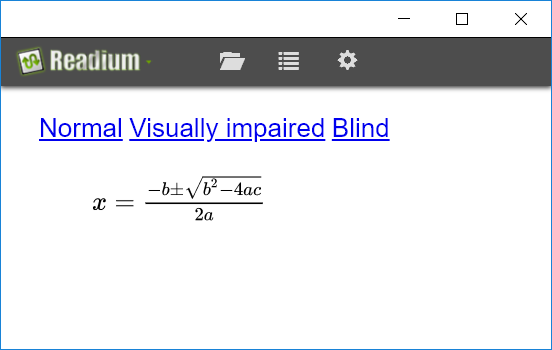
\includegraphics[width=\linewidth*2/3]{figures/EquationNo.PNG}
	\caption{Equation in 'Normal' mode}
	\label{fig:equation_normal}
\end{figure}

\begin{figure}[H]
	\centering
	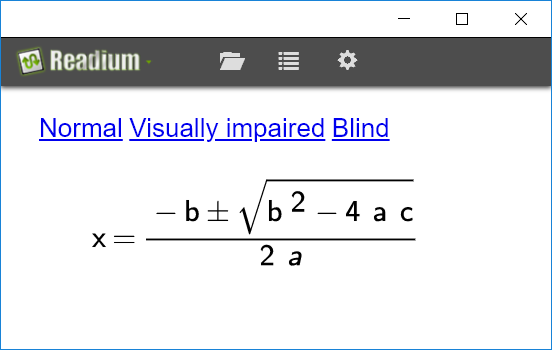
\includegraphics[width=\linewidth*2/3]{figures/EquationVi.PNG}
	\caption{Equation in 'Visual impairment' mode}
	\label{fig:equation_viimp}
\end{figure}



In the normal version the default display style is used, which uses a serif font and a combination of italicized and unitalicized letters, as shown in figure~\ref{fig:equation_normal}. Serif fonts are not suitable in the visually impaired version, so a sans serif had to be chosen. At first the font was changed in the CSS. This unfortunately resulted in the text not scaling properly, and therefore some characters were not properly spaced. The root symbol also wasn't displayed clearly. Instead the mstyle attribute of MathML had to be changed to sans serif which resulted in figure~\ref{fig:equation_viimp}. The mstyle attribute can not be changed in CSS, it has to be inserted into every math element.

\begin{figure}[H]
	\centering
	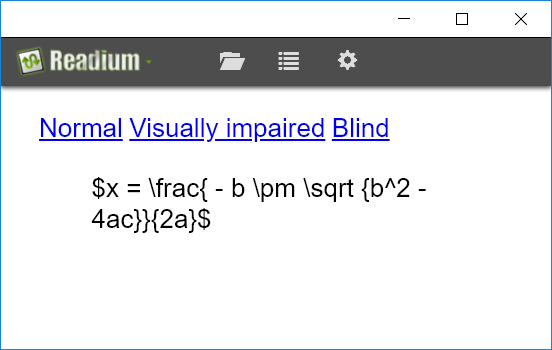
\includegraphics[width=\linewidth*2/3]{figures/EquationBl.PNG}
	\caption{Equation in 'Blind' mode}
	\label{fig:equation_blind}
\end{figure}

In the blind version, the text has to appear as LaTeX code. Much like the alternative text for images, it will appear as a separate paragraph enclosed in \lstinline{<p>}  tags. To signify that it is code, it has to be surrounded by \$ signs, as shown in figure~\ref{fig:equation_blind}. The math element is in a \lstinline{<div>} with CSS class "math", which is hidden in the blind version.




\begin{figure}
	
	\begin{lstlisting}
	<figure>
		<div role="math" class="math">
		<math xmlns="http://www.w3.org/1998/Math/MathML" id="Formula" title="Quadratic Formula" alttext="{x=\frac{-b\pm\sqrt{b^2-4ac}}{2a}}">
			<mstyle>
			<semantics>

			<mrow>
			<mi>x</mi>
			<mo>=</mo>
			<mfrac>
			<mrow>
			<mrow>
			<mo>-</mo>
			<mi>b</mi>
			</mrow>
			<mo>%*±</mo>*)
			<msqrt>
			<mrow>
			<msup>
			<mi>b</mi>
			<mn>2</mn>
			</msup>
			<mo>-</mo>
			<mrow>
			<mn>4</mn>
			<mo></mo>
			<mi>a</mi>
			<mo></ mo>
			<mi>c</mi>
			</mrow>
			</mrow>
			</msqrt>
			</mrow>
			<mrow>
			<mn>2</mn>
			<mo></mo>
			<mi>a</mi>
			</mrow>
			</mfrac>
			</mrow> 
			
			</semantics>
			</mstyle>
	</math>
	</div>

	<p class="transparent">
		$x = \frac{ - b \pm \sqrt {b^2 - 4ac}}{2a}$
	</p>

</figure>
	\end{lstlisting}
	
\caption{Code of figures \ref{fig:equation_normal} and \ref{fig:equation_blind}}
	\label{fig:math_code}
\end{figure}

\begin{figure}
	
	\begin{lstlisting}
		<mstyle scriptsizemultiplier="1" lspace="20%" rspace="20%" mathvariant="sans-serif">
	\end{lstlisting}
	\caption{Addition to the code shown in \ref{fig:math_code} for the visually impaired version to make the formula appear as sans serif and not in italics}
		\label{fig:math_vi_code}
\end{figure}



\chapter{Evaluation EPUB Standard}
\label{ch:Evaluation EPUB Standard}

\begin{figure}[h]

	\begin{minipage}{0.5\textwidth}
		\centering
		\fbox{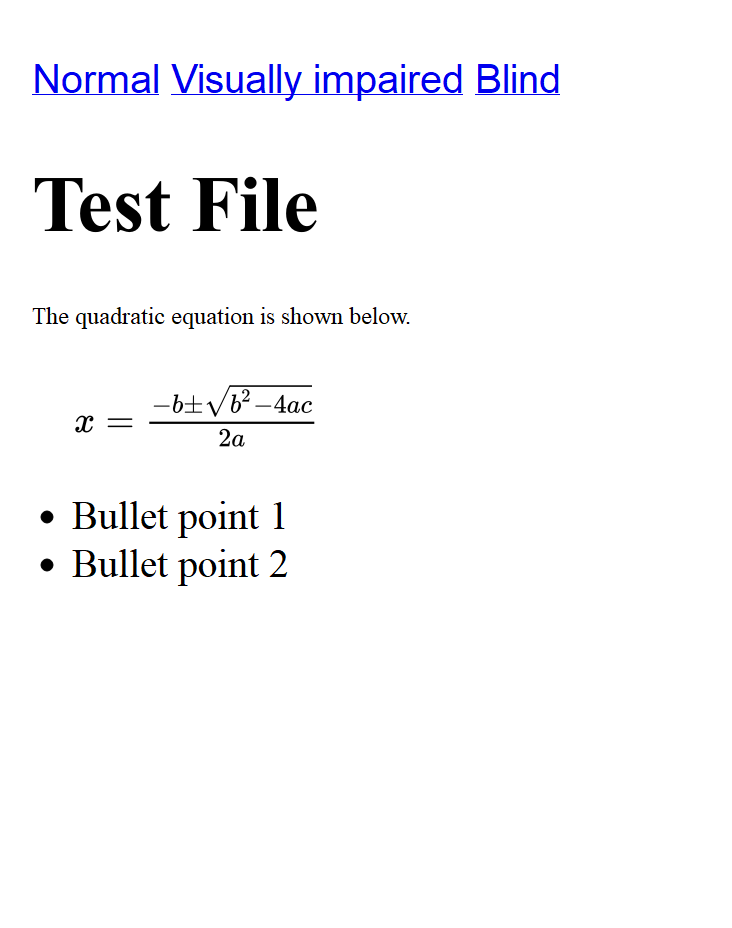
\includegraphics[height=10cm]{figures/ExampleEPUB1.png}}
	\end{minipage}\hfill
	\begin{minipage}{0.5\textwidth}
		\centering
		\fbox{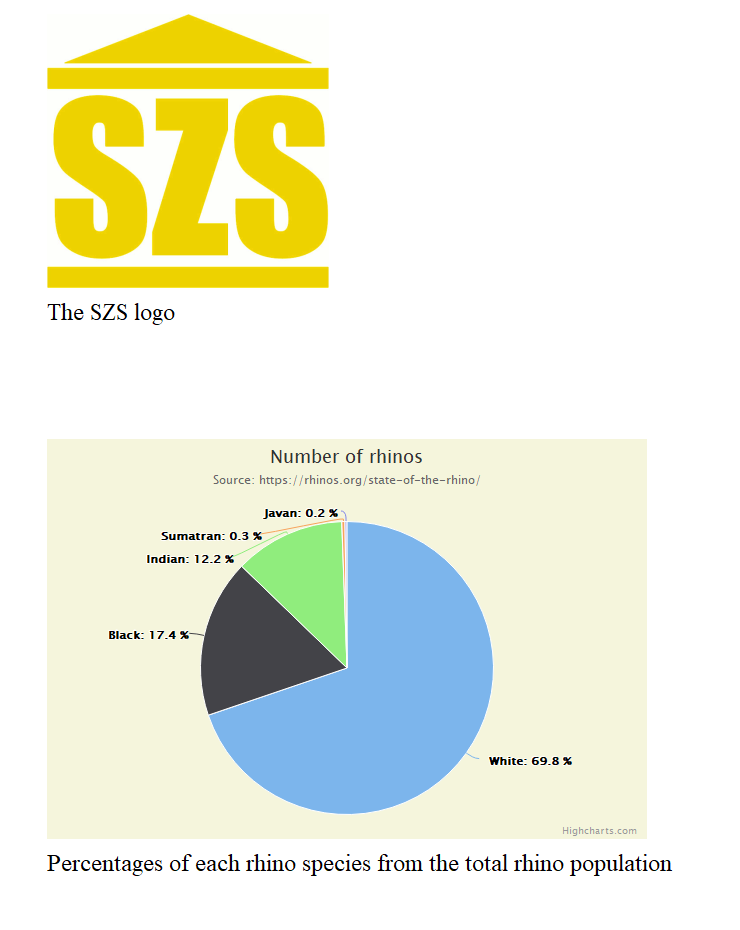
\includegraphics[height=10cm]{figures/ExampleEPUB2.png}}
	\end{minipage}

	\caption{Example EPUB which will be tested}
	\label{fig:exampleEPUB}
\end{figure}

%This chapter is going to present an evaluation of how documents of the new standard were displayed in several EPUB reading systems. The test document has the same content that will be in both versions of the new standard. The CSS version is shown in figure \ref{fig:exampleEPUB}. It is shown in dual column mode so that the whole document can be shown at once. Actually the SZS logo is followed by the graph, so that is the proper reading order. The file has following content:
This chapter presents the evaluation of both new document standards developed for this thesis. A test document in both standards was created (the CSS version is shown in figure 4.1). To test the all new functionalities, the documents contain the following elements:
\begin{enumerate}
	\item A heading of level 1
	\item Standard text
	\item A figure with a MathML equation
	\item A short list
	\item A figure with a PNG
	\item A figure with a SVG
\end{enumerate}

%All of these features are important to keep the document accessible. It is vital to have both a PNG and a SVG to test if a SVG can be displayed. Unlike PNG, they are not a standard format so they might not be supported. The operating systems tested are Android 8.1, iOS 11.2 and Windows 10.

All of these features are important to keep the document accessible. It is vital to have both a PNG and a SVG to test if a SVG can be displayed. Unlike PNG, it are not a standard format so it might not be supported. The standards were tested on several devices and tools running on Android 8.1, iOS 11.2 and Windows 10.
The following parts present the individual tools and discuss the pros and cons. The last part is a conclusion with a summary. 


\section{Reading systems on Android}
	
\subsection{Reasily}

\begin{figure}[h]
	
	\begin{minipage}{0.47\textwidth}
		\centering
		\fbox{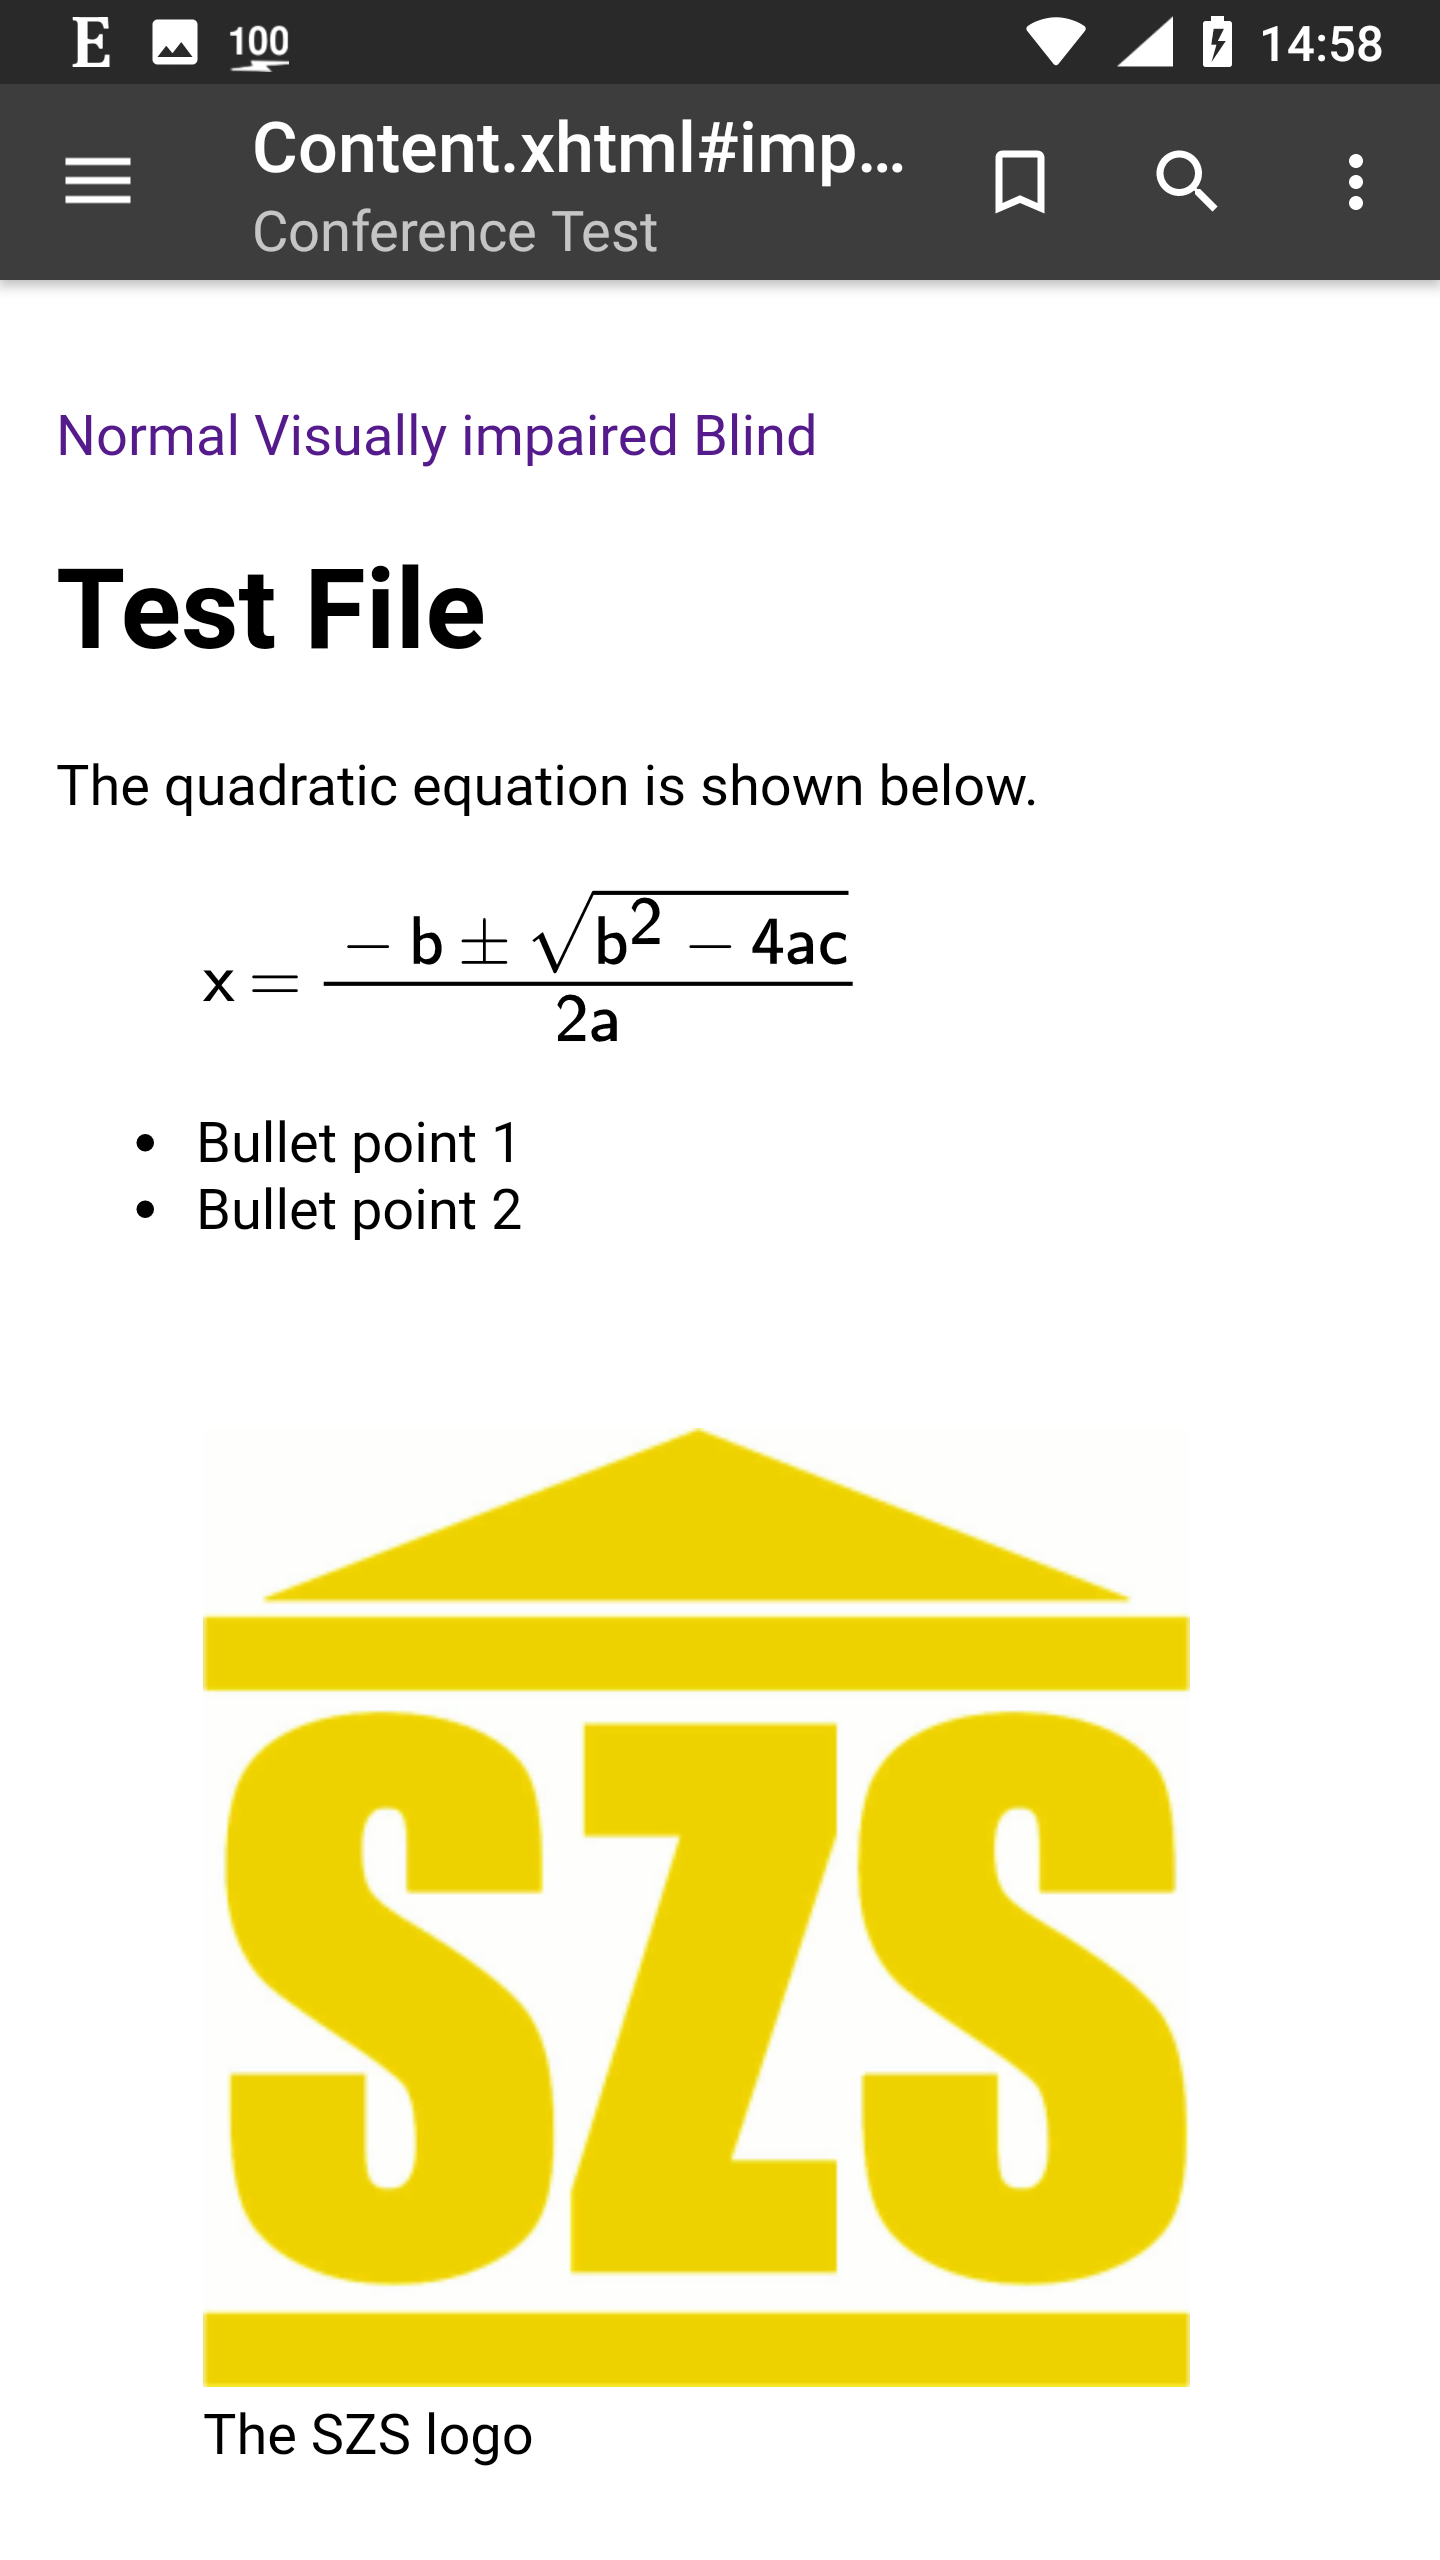
\includegraphics[width=\linewidth]{figures/ReasilyVi1.png}}
	\end{minipage}\hfill
	\hspace{0.05cm}
	\begin{minipage}{0.47\textwidth}
		\centering
		\fbox{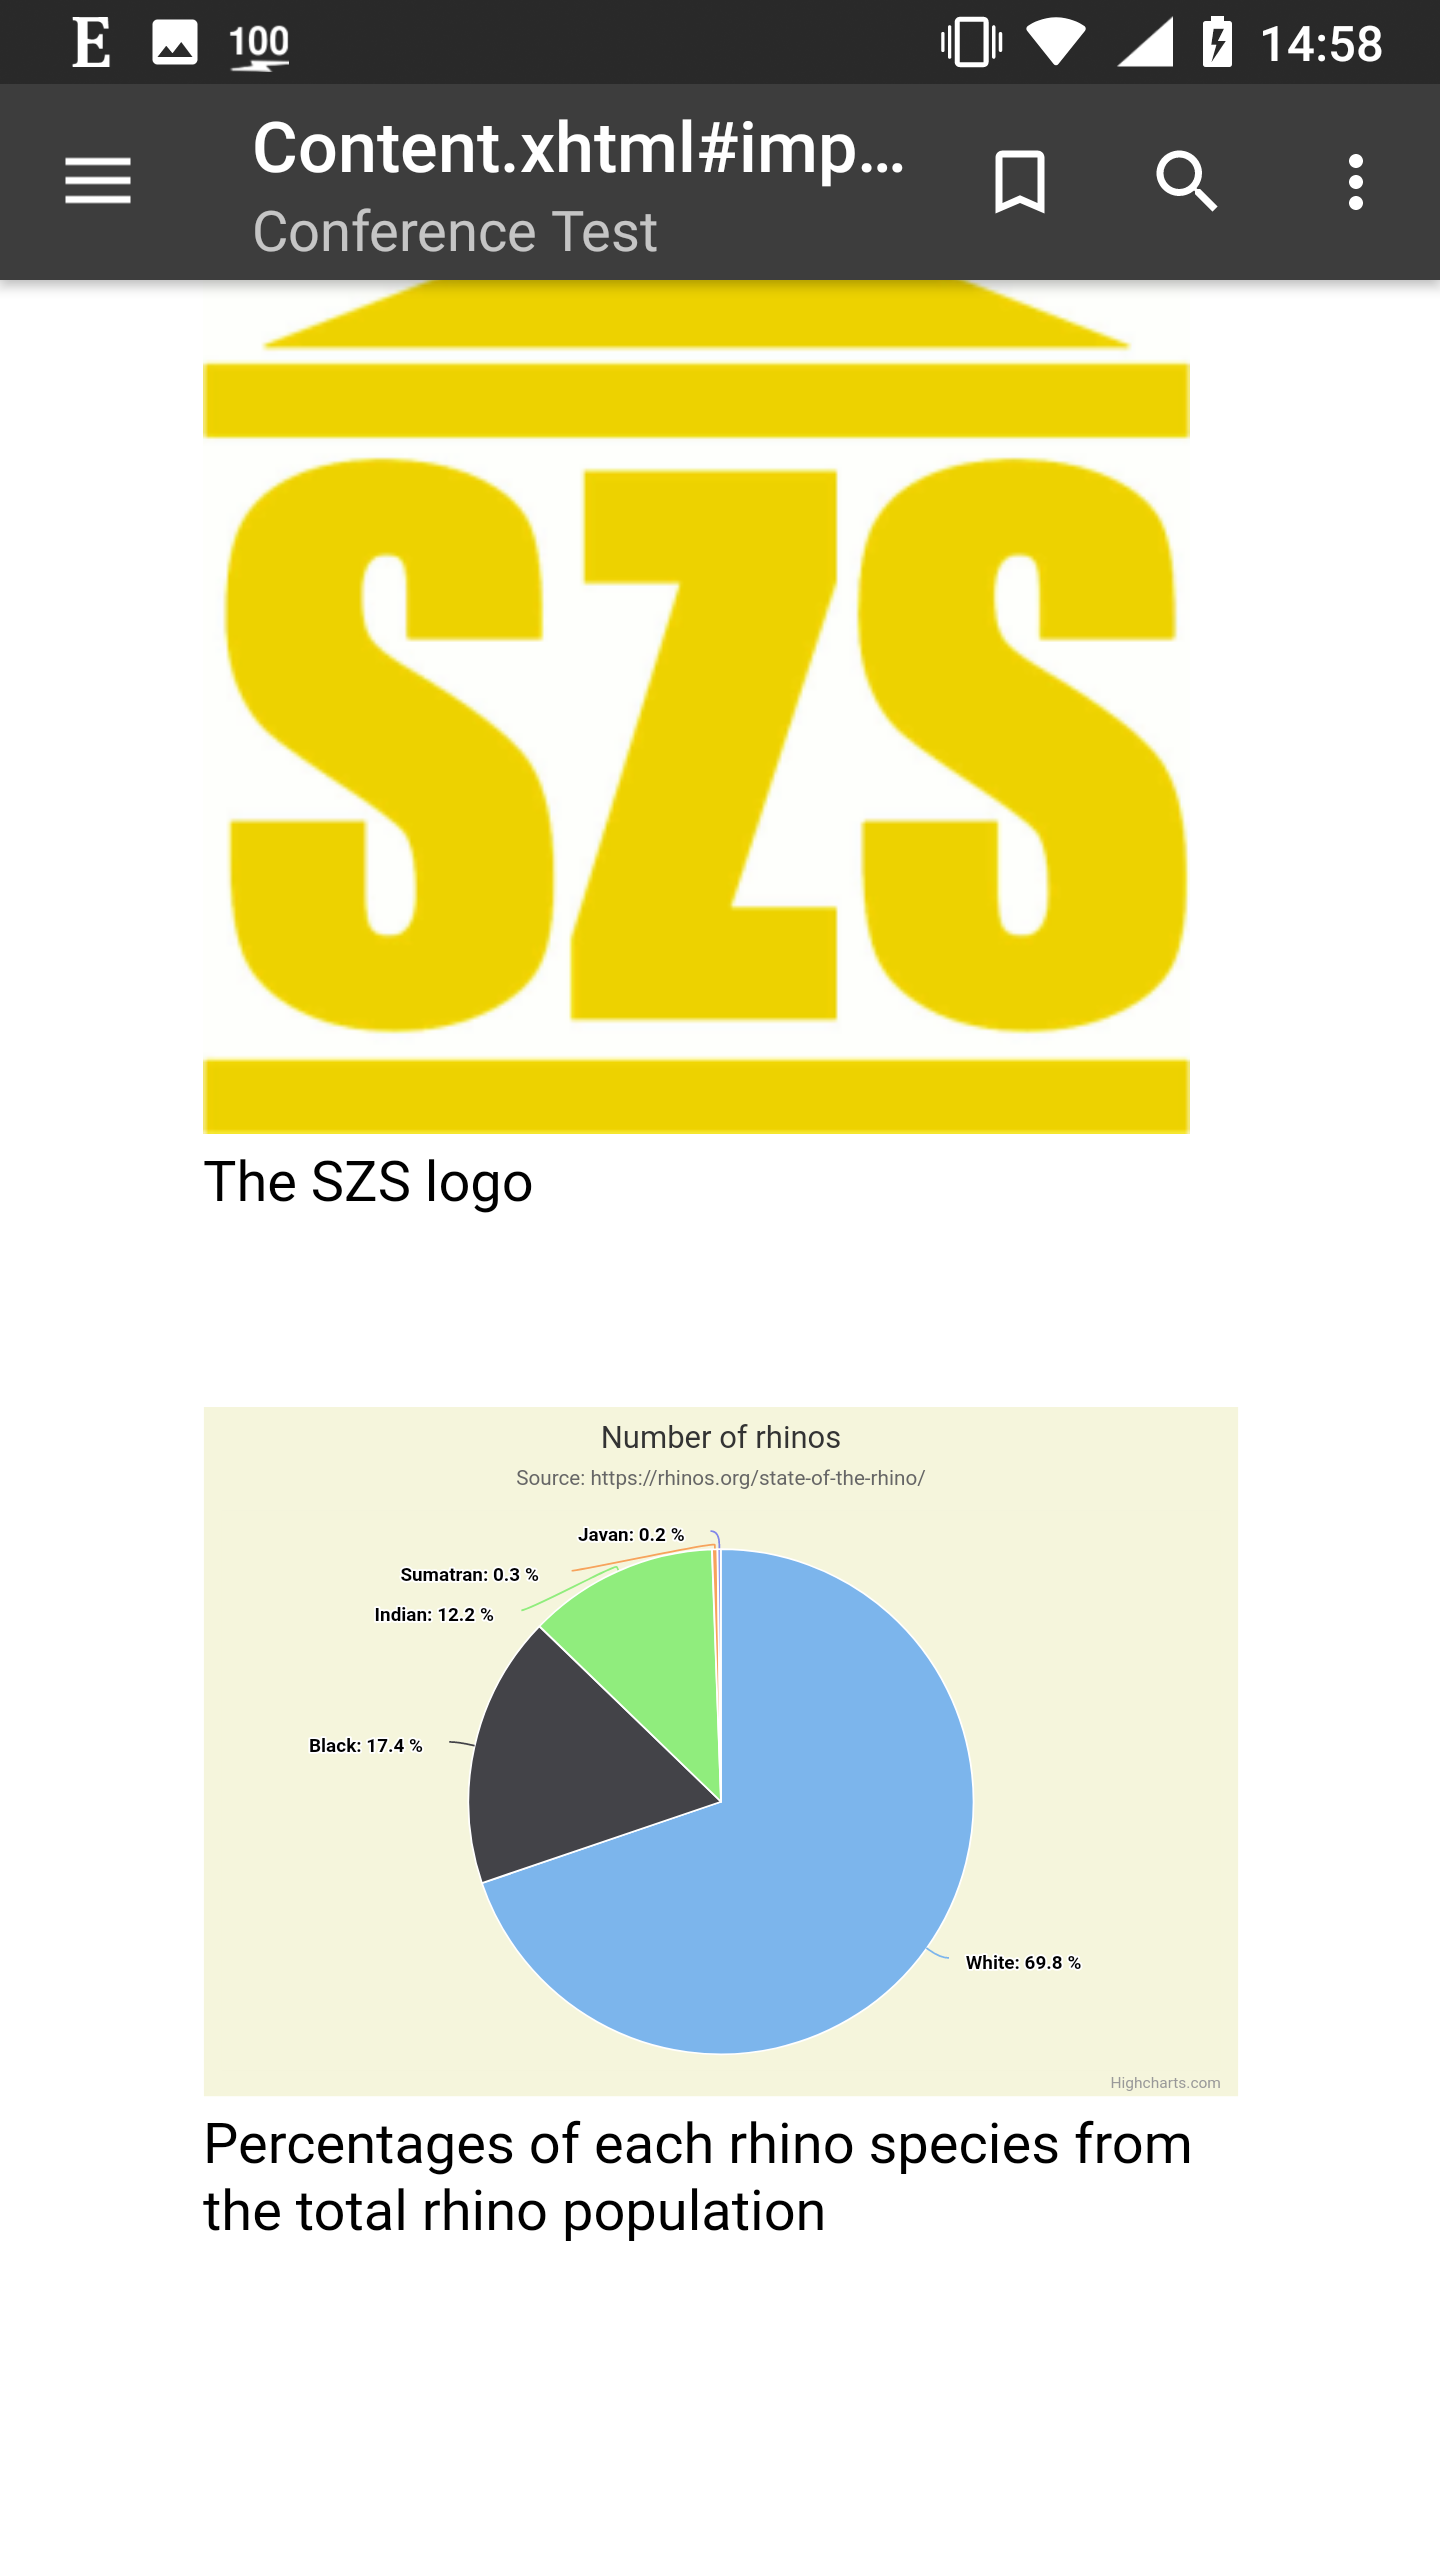
\includegraphics[width=\linewidth]{figures/ReasilyVi2.png}}
	\end{minipage}
	
	\caption{The visually impaired display style in Reasily}
	\label{fig:reasilyVi}
\end{figure}
Reasily is an Android EPUB reading app which states that it has support for several EPUB 3 features such as MathML and media overlay for read aloud books\footnote{https://play.google.com/store/apps/details?id=com.gmail.jxlab.app.reasily}. While the JavaScript standard does not switch versions correctly, the CSS version does. The normal display style is shown much like in figure \ref{fig:exampleEPUB}. All elements are shown as desired. Each of the figures with MathML, PNG and SVG are displayed properly. 

\begin{comment}
\begin{figure}[h]
	\begin{minipage}{0.5\textwidth}
		\centering
		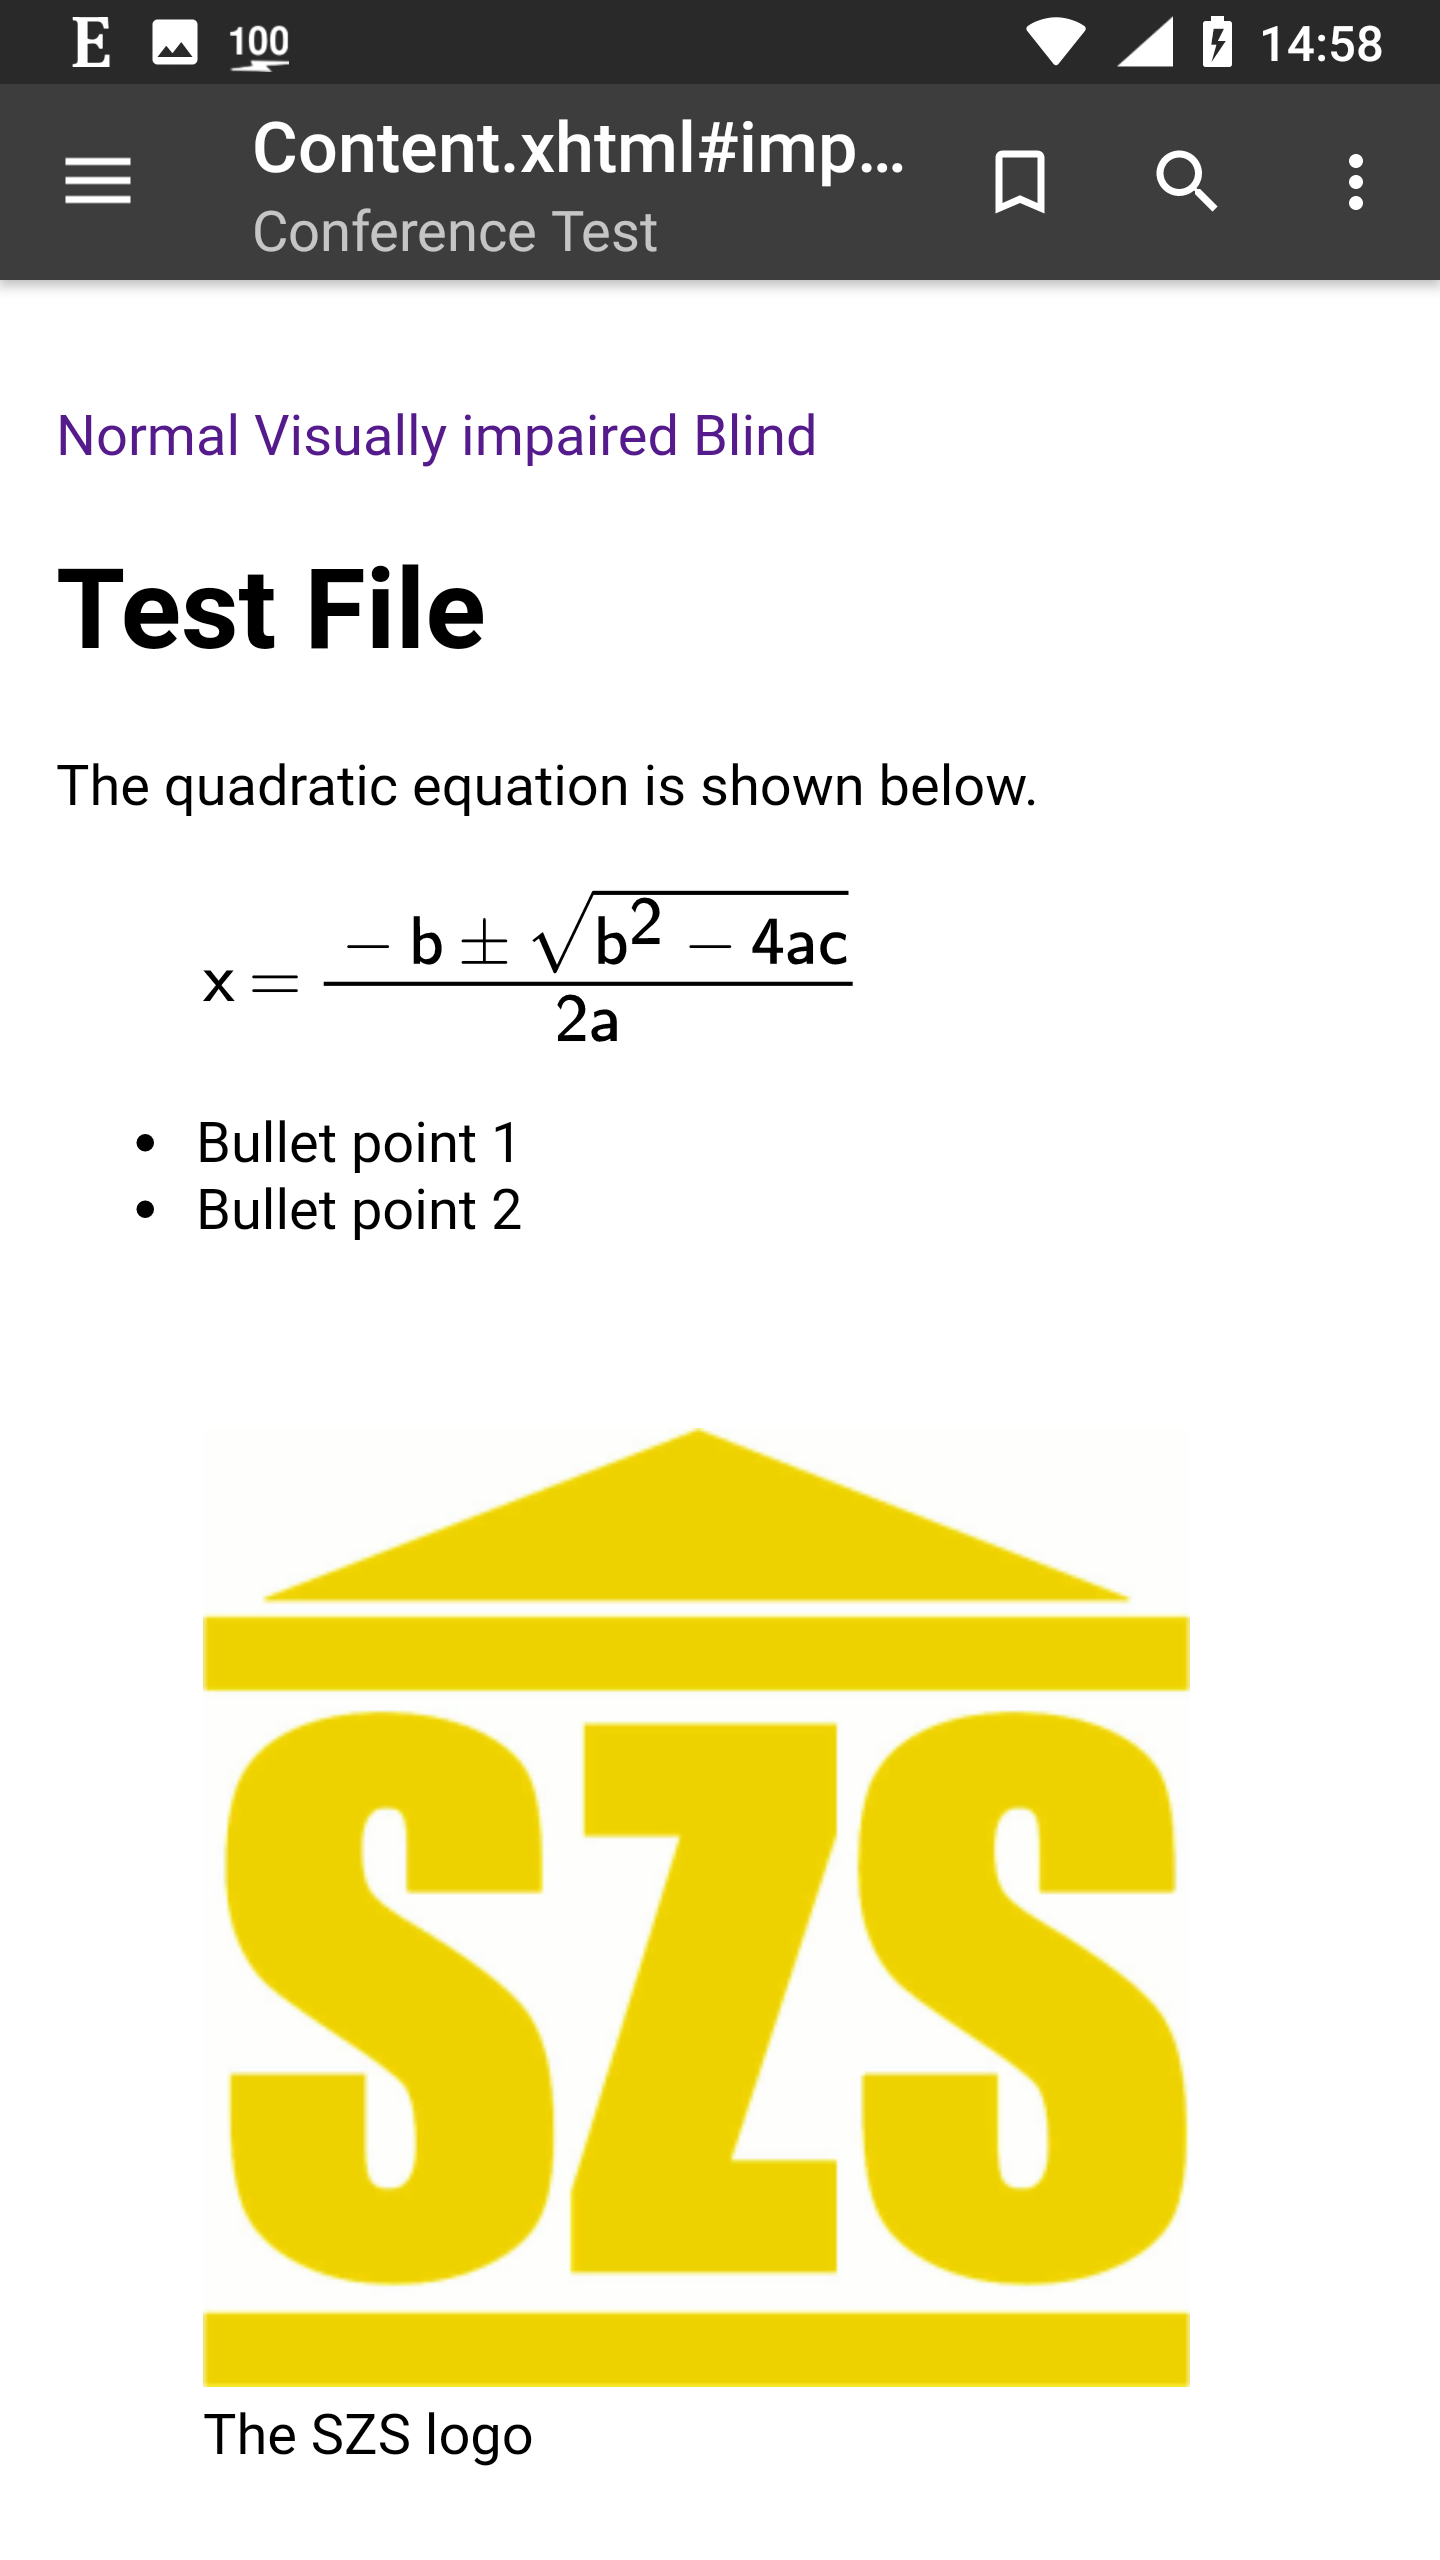
\includegraphics[width=\linewidth]{figures/ReasilyVi1.png}
	\end{minipage}\hfill
	\begin{minipage}{0.5\textwidth}
		\centering
		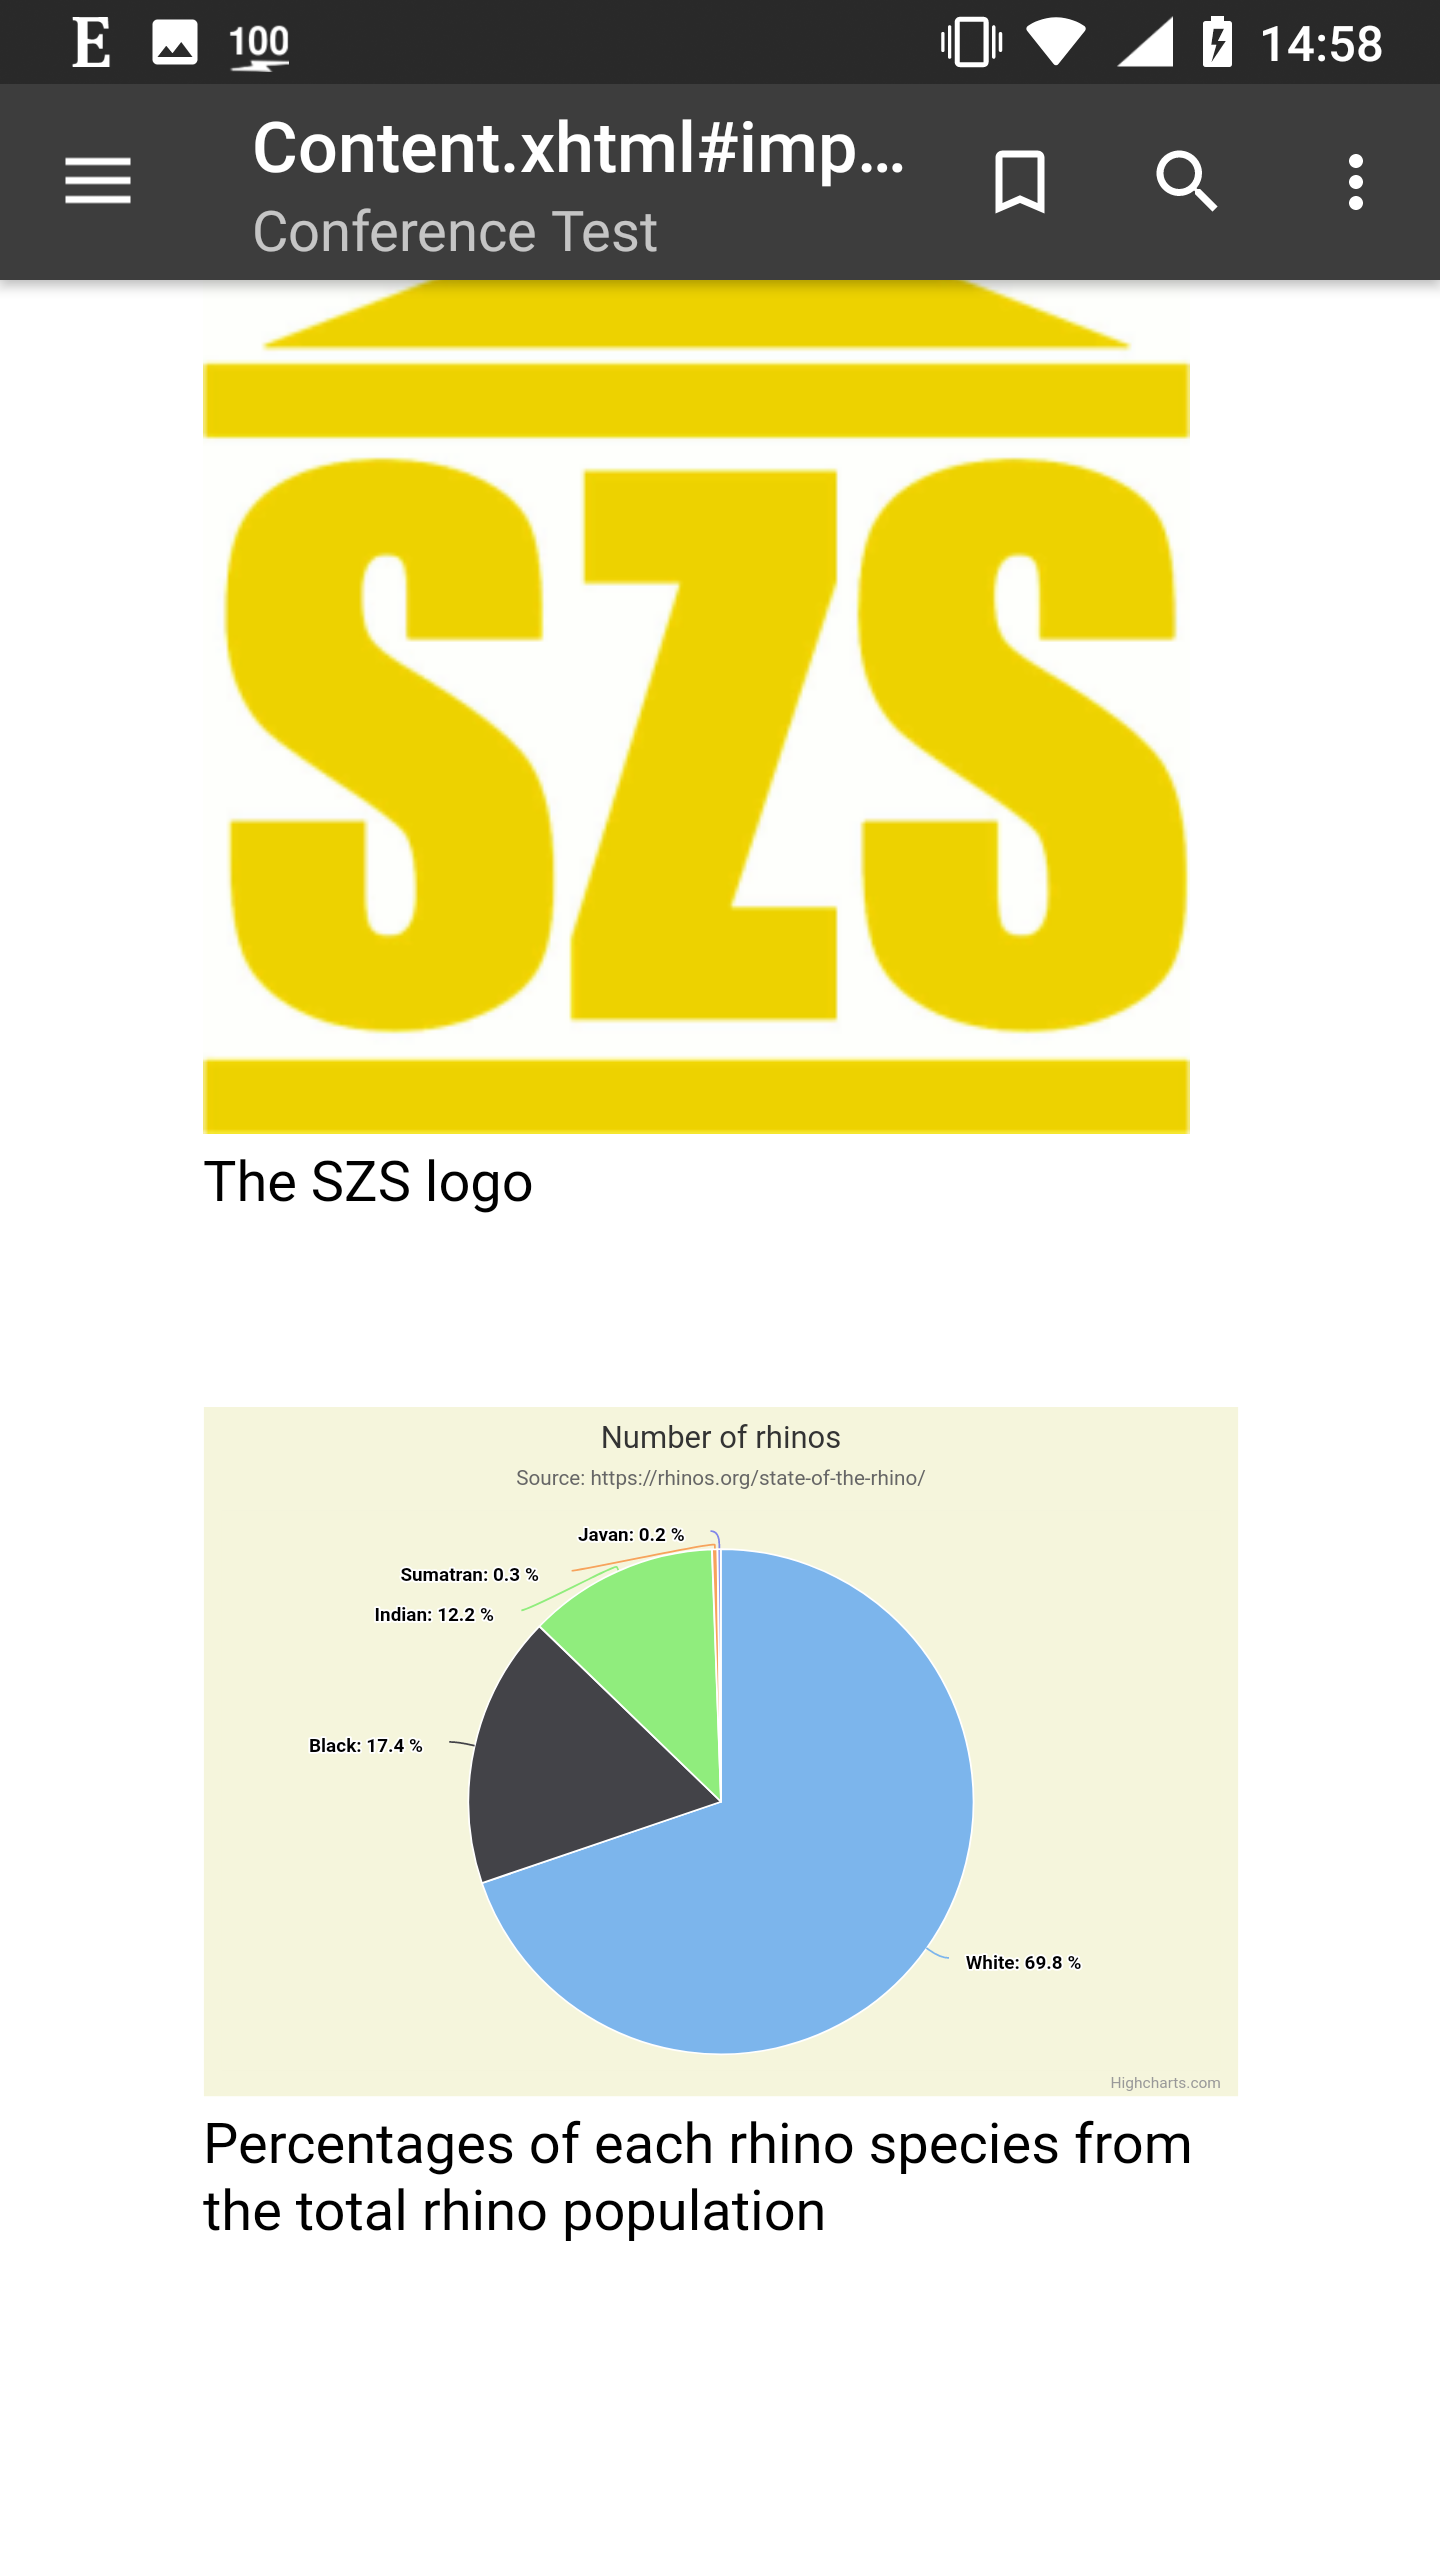
\includegraphics[width=\linewidth]{figures/ReasilyVi2.png}
	\end{minipage}
	\caption{The visually impaired display style in Reasily}
	\label{fig:reasilyVi2}
\end{figure}
\end{comment}

The visually impaired display style in figure \ref{fig:reasilyVi} is also shown properly, with the MathML equation using a sans serif font. The blind display style in figure \ref{fig:reasilyBl} is shown correctly, with the equations and images showing the alternative text with the appropriate tags. Furthermore, Reasily supports the preinstalled screen reader of Android, TalkBack, and elements such as the heading of level 1 are identified properly.

\begin{figure}[H]
	\centering
	\fbox{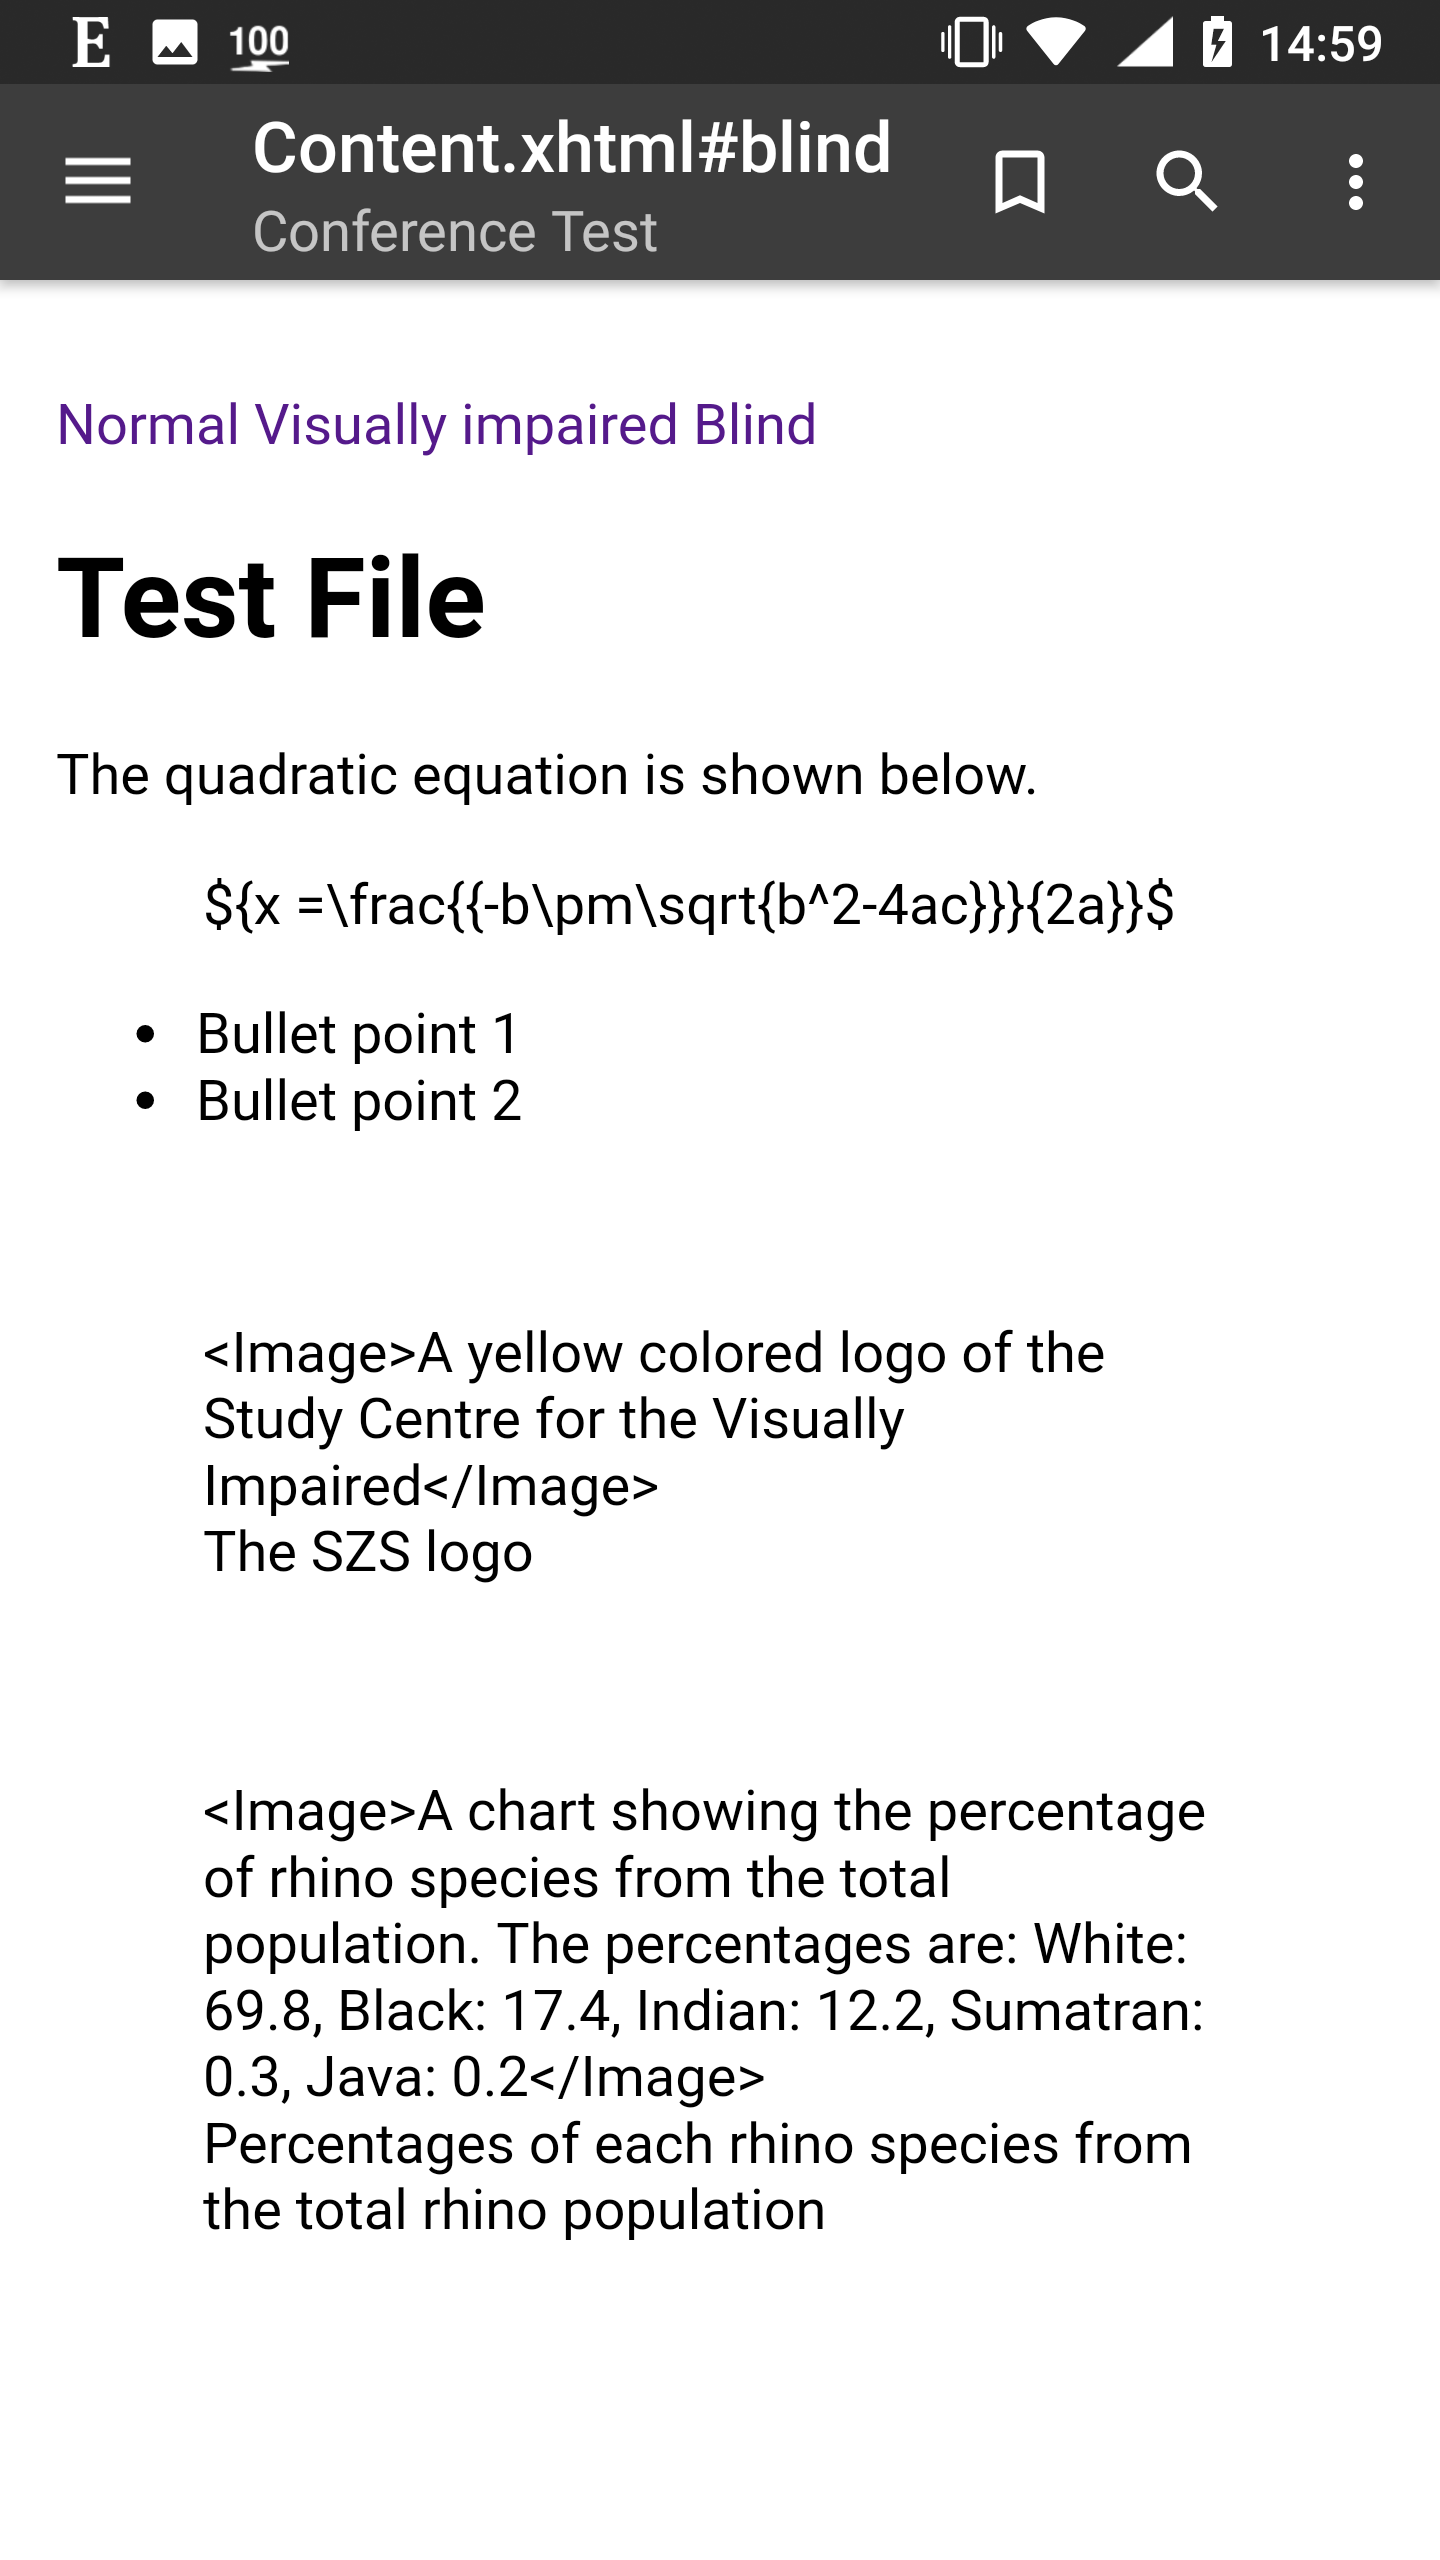
\includegraphics[width=\linewidth/3]{figures/ReasilyBl.png}}
	\caption{The blind display style in Reasily}
	\label{fig:reasilyBl}
\end{figure}

\subsection{Unusable reading systems}

\subsubsection{Tolino}
Tolino is a cooperation of several large German booksellers to create a unified E-Book reading device\footnote{https://mytolino.de/tolino-kooperationen-und-vertrieb/}. There is a Tolino app on Android which can be used to see how well the EPUBs following the document standard run on the Tolino reading device family, as they likely share similar technology. However, the Android app is more powerful than the Tolino reading devices as it can also show color beyond greyscale. As seen in figure \ref{fig:tolino}, the app is unable to display MathML. Furthermore, it does not show the PNG file, which should actually be supported, as other files with images are displayed properly. This is due to the image being enclosed in a figure element. If it is not in one, the image is displayed correctly. 

\begin{figure}[h]
	\centering
	\fbox{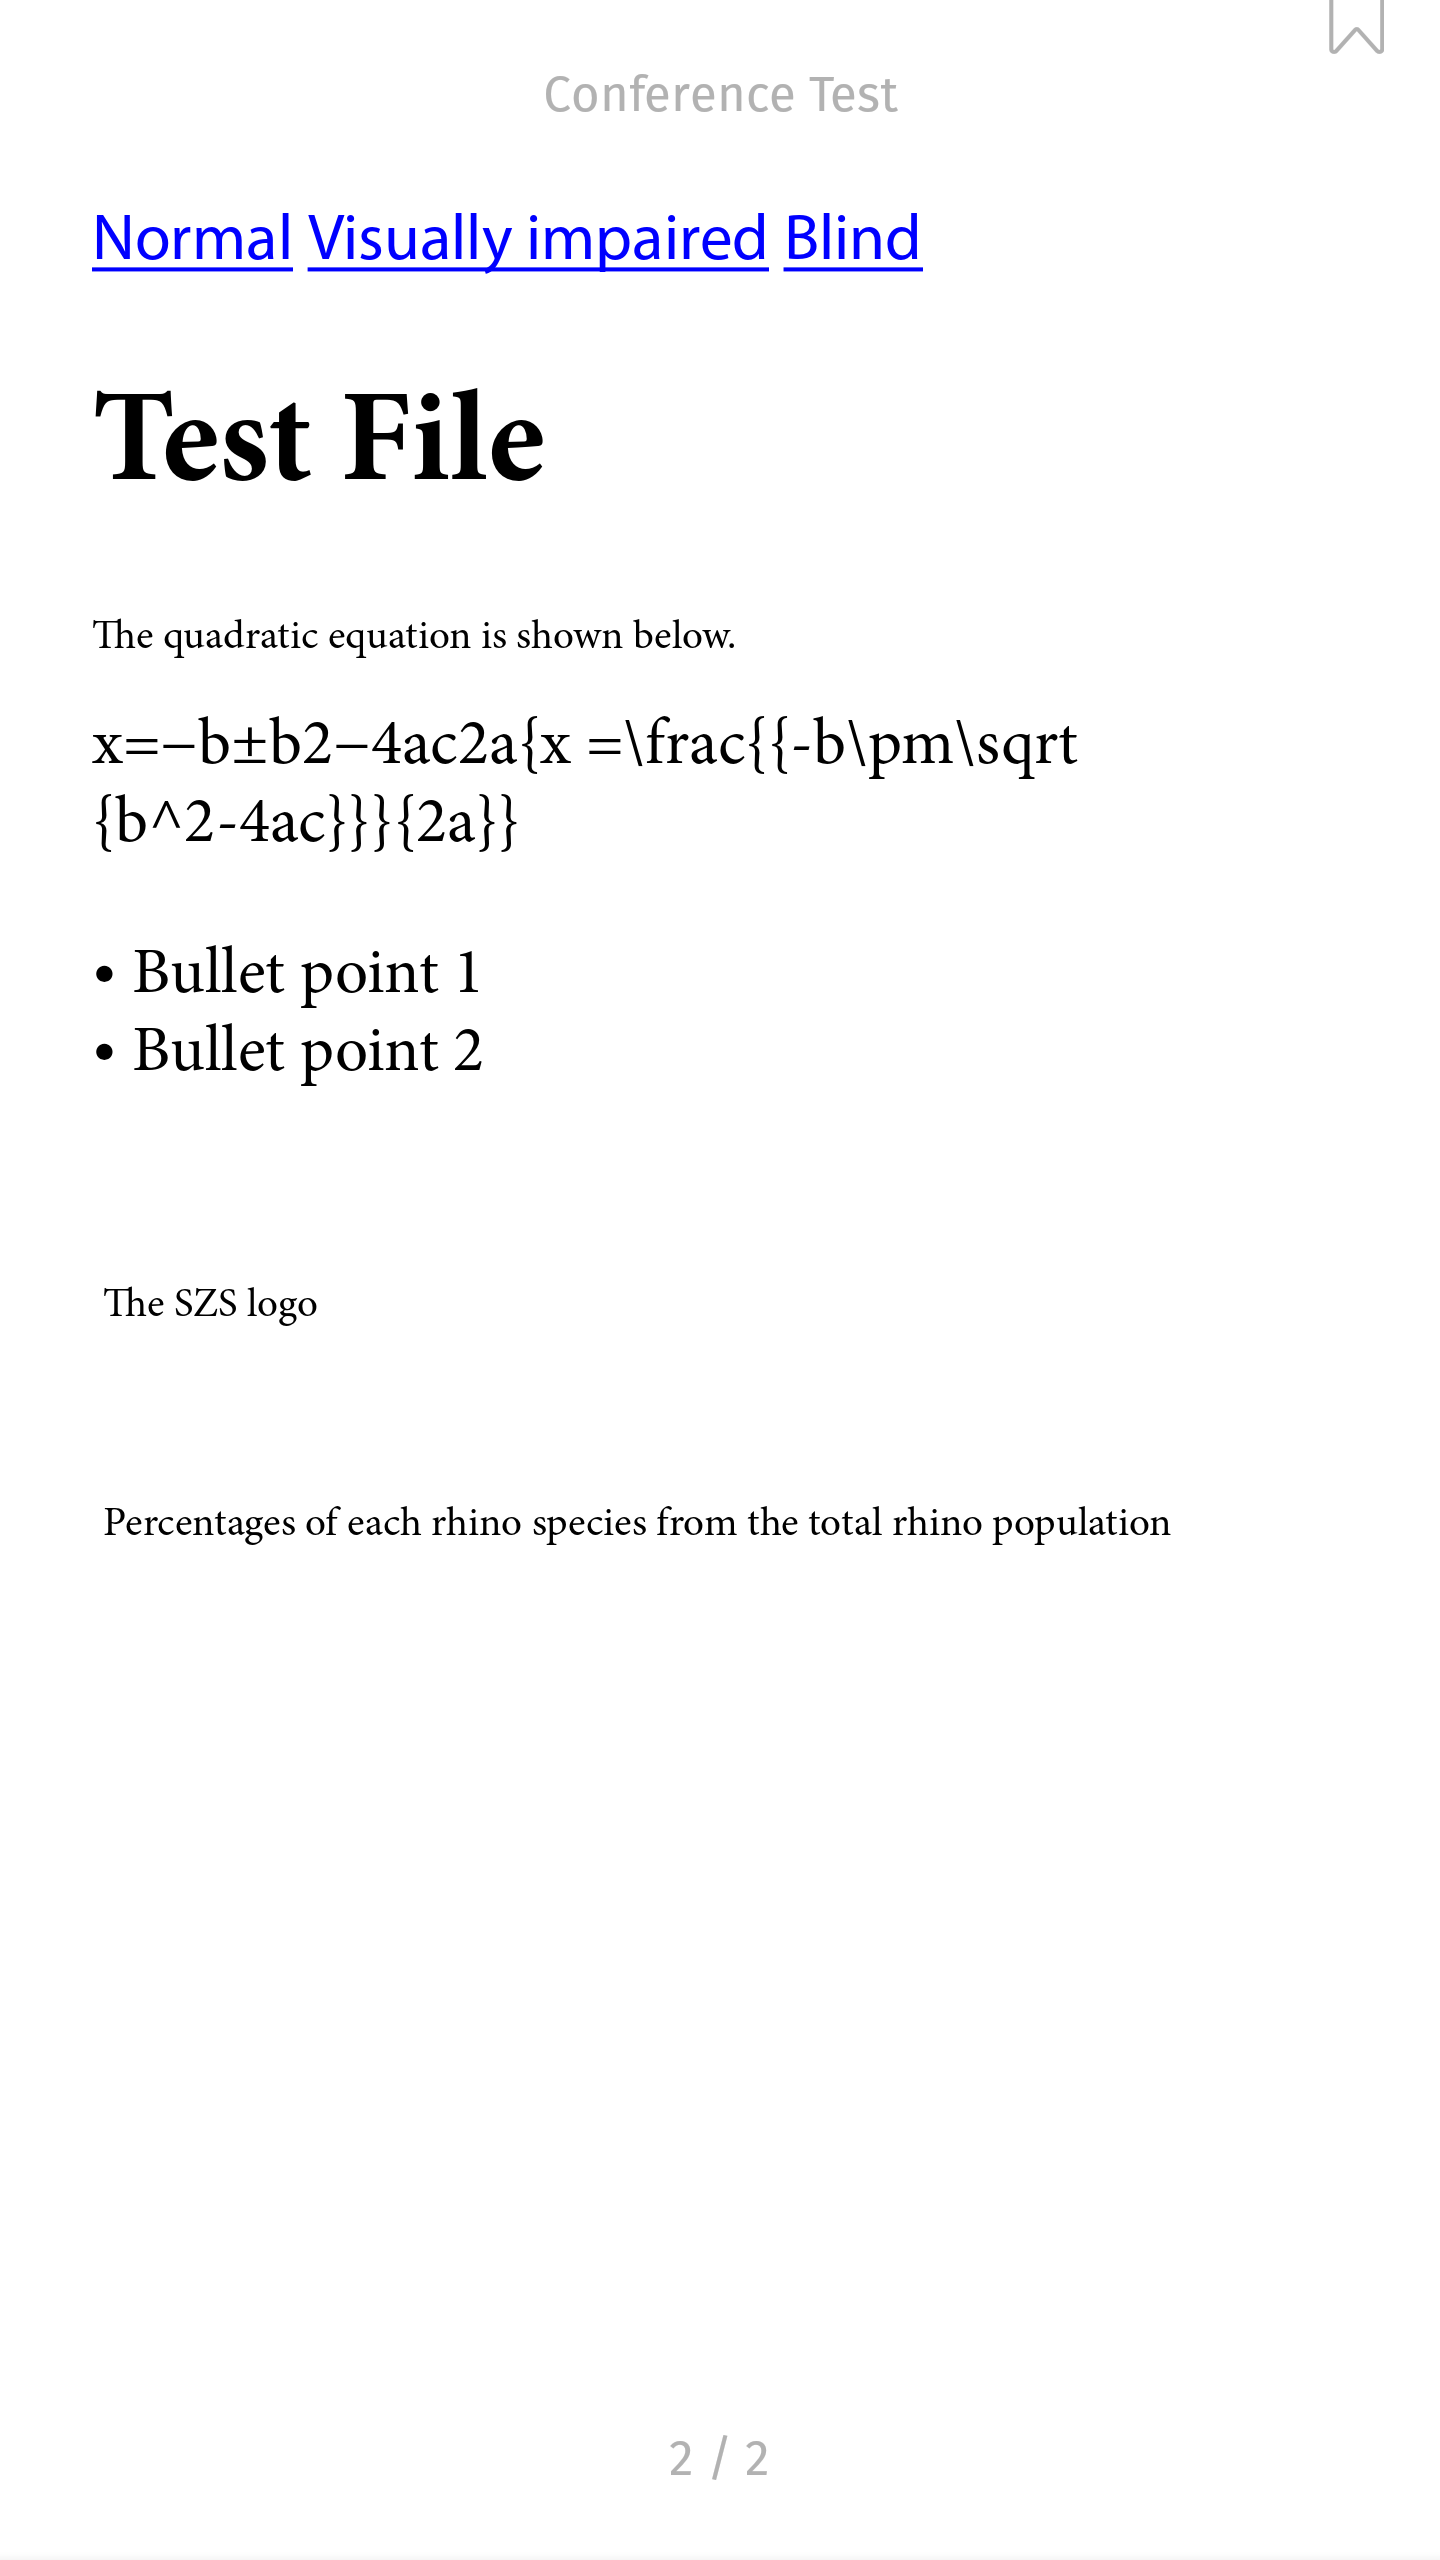
\includegraphics[width=\linewidth/3]{figures/Tolino.png}}
	\caption{EPUB of the CSS standard shown in Tolino}
	\label{fig:tolino}
\end{figure}

The switching mechanism does not work with both the CSS and JavaScript versions. This means that the Tolino app does not support scripting and also does  not support CSS 3. TalkBack also does not work with the Tolino app.

\subsubsection{Gitden Reader}

Gitden Reader is an Android app\footnote{https://play.google.com/store/apps/details?id=com.gitden.epub.reader.app} with MathML support. It does not support both of the switching mechanisms, but does display the MathML, PNG and SVG properly. It supports TalkBack, but the equation is not identified properly and not read aloud.

\subsubsection{FBReader}
\begin{figure}[H]
	\centering
	\fbox{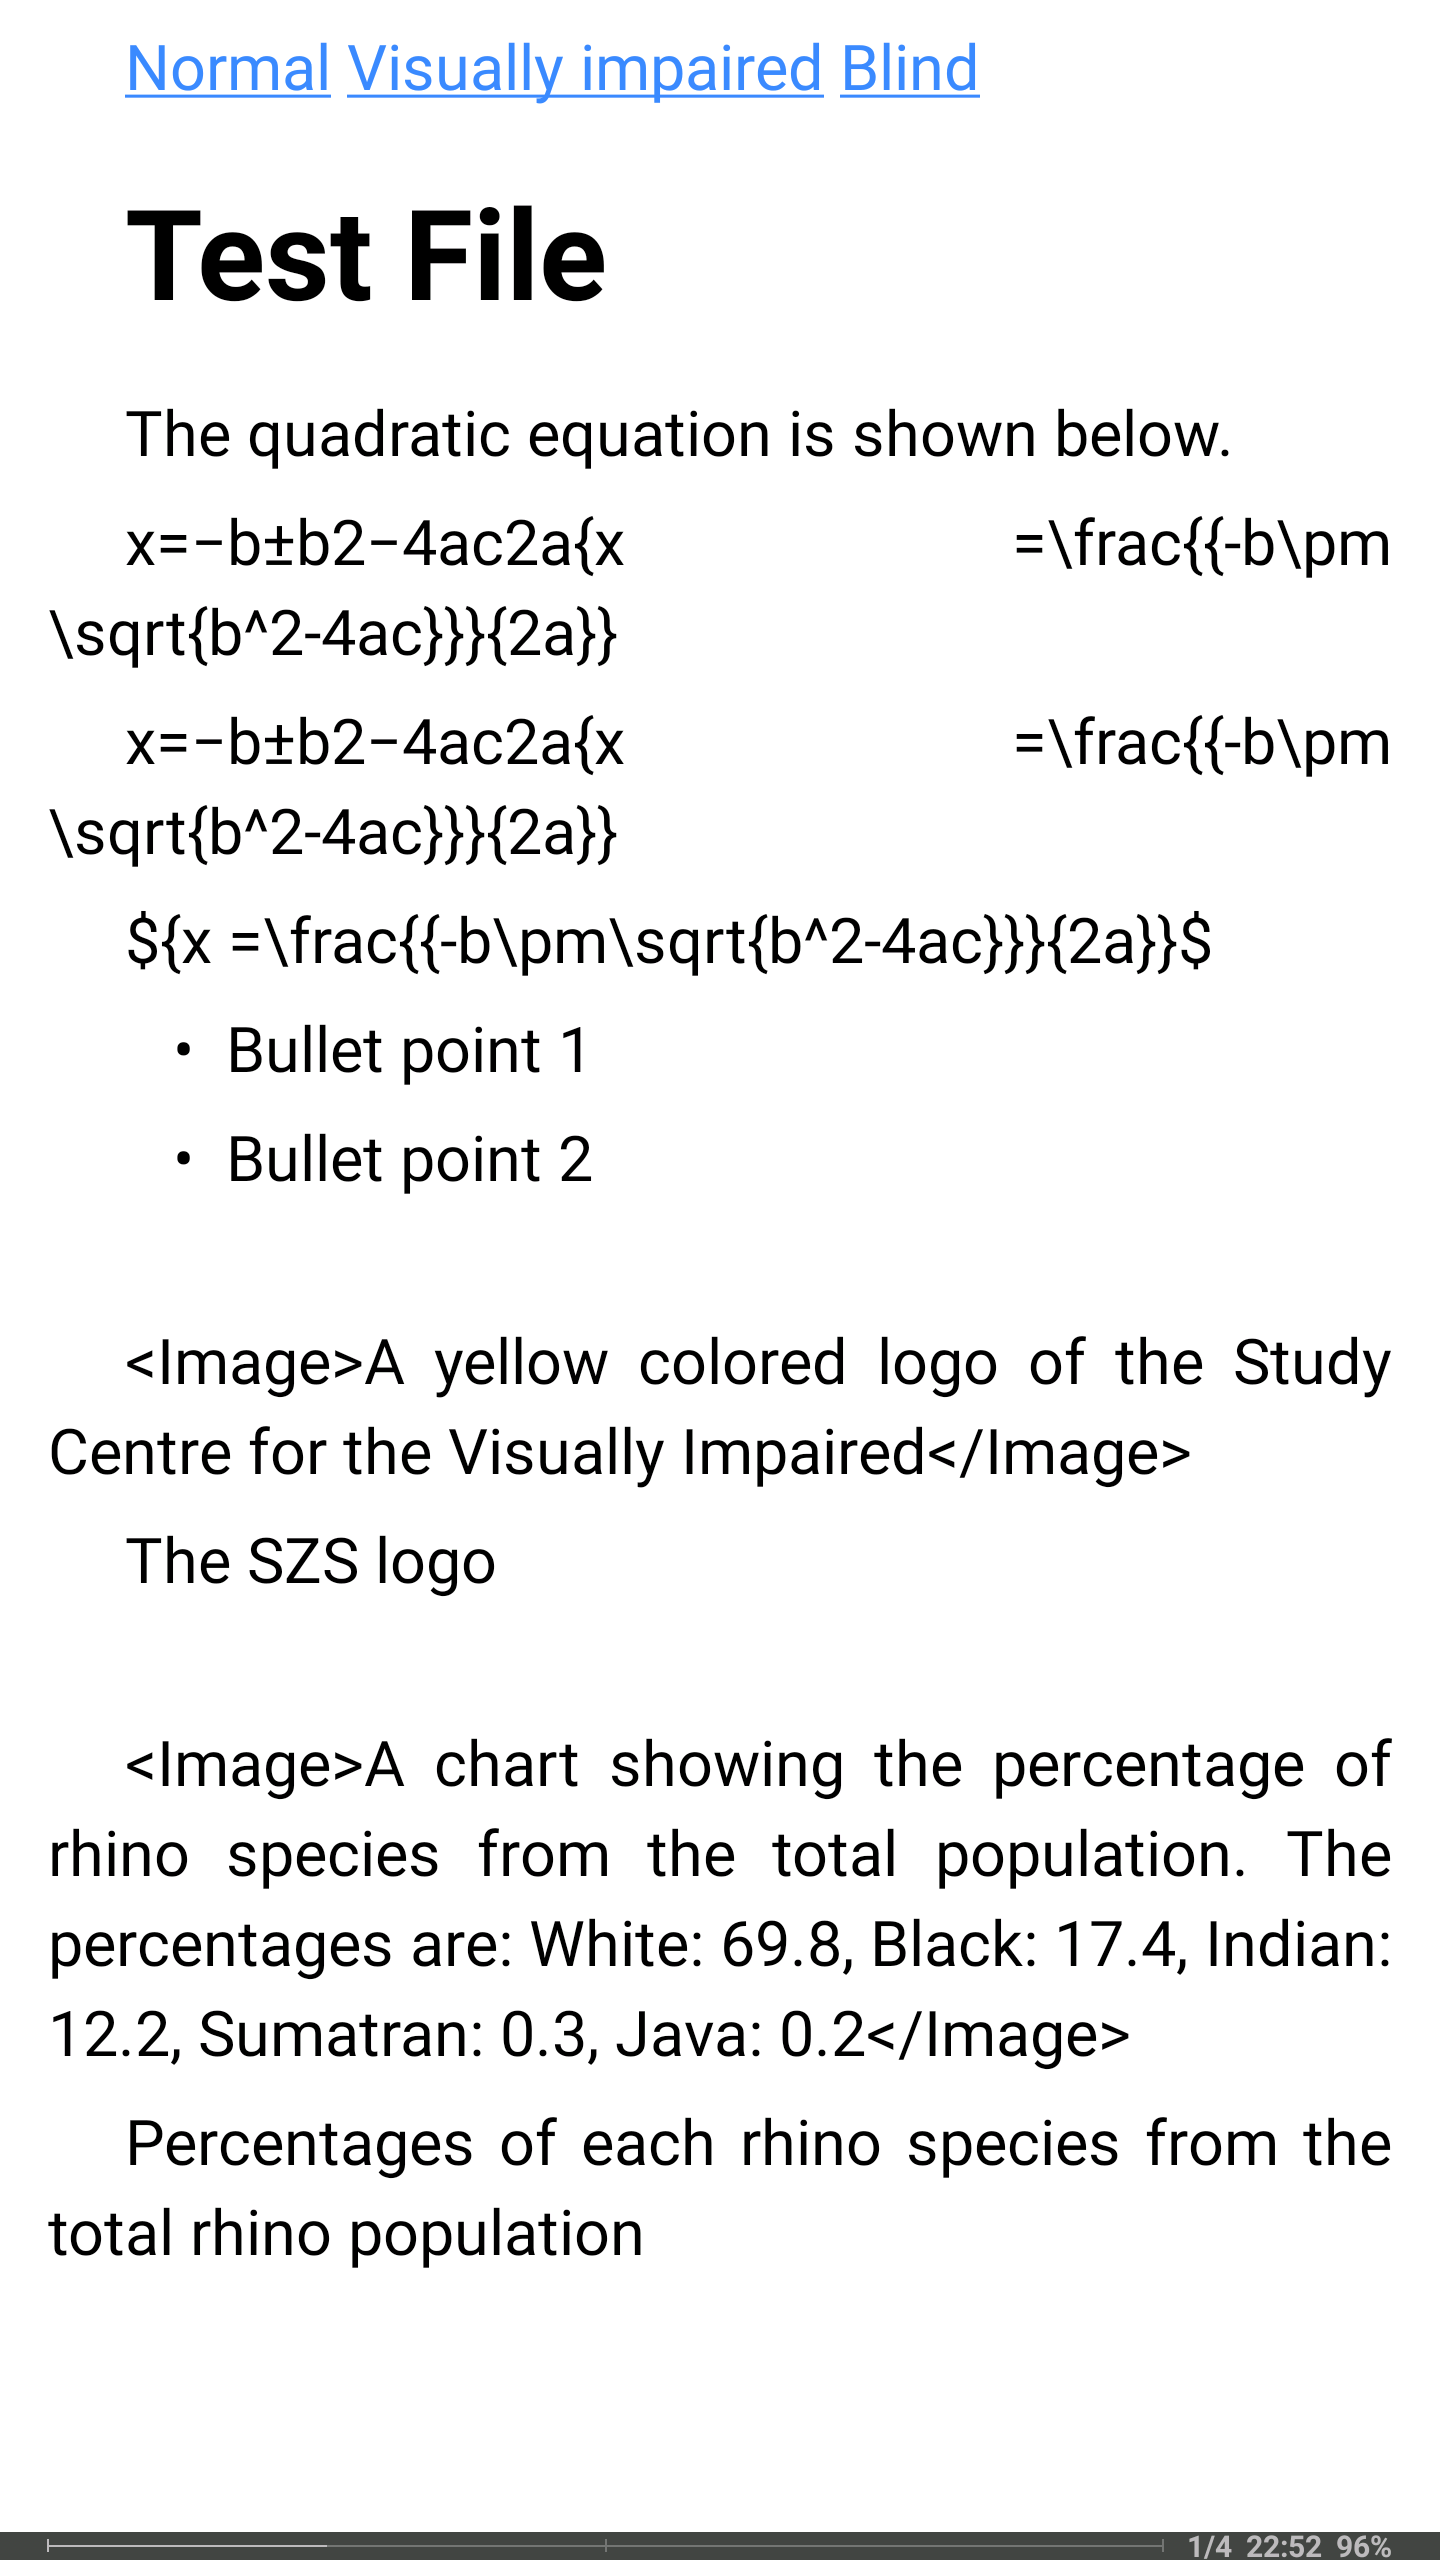
\includegraphics[width=\linewidth/3]{figures/fbreader.png}}
	\caption{The CSS file in FBReader}
	\label{fig:fbreader}
\end{figure}
FBReader is a popular E-Book reader available on Android\footnote{https://play.google.com/store/apps/details?id=org.geometerplus.zlibrary.ui.android}. Both CSS and JavaScript switching do not function as intended. Furthermore, none of the MathML, PNG and SVG are shown properly. The MathML first shows the equation not rendered properly and then annotation which should actually be hidden. One interesting observation is that elements which are supposed to be hidden, such as the text between the \lstinline|<Image>| tags, are shown. The CSS file even has three pages showing the same page as shown in figure \ref{fig:fbreader}, only the links at the top are missing. Thus it is likely that FBReader does not support certain CSS features such as hiding elements.

\subsubsection{UB Reader}

\begin{figure}[H]
	\centering
	\fbox{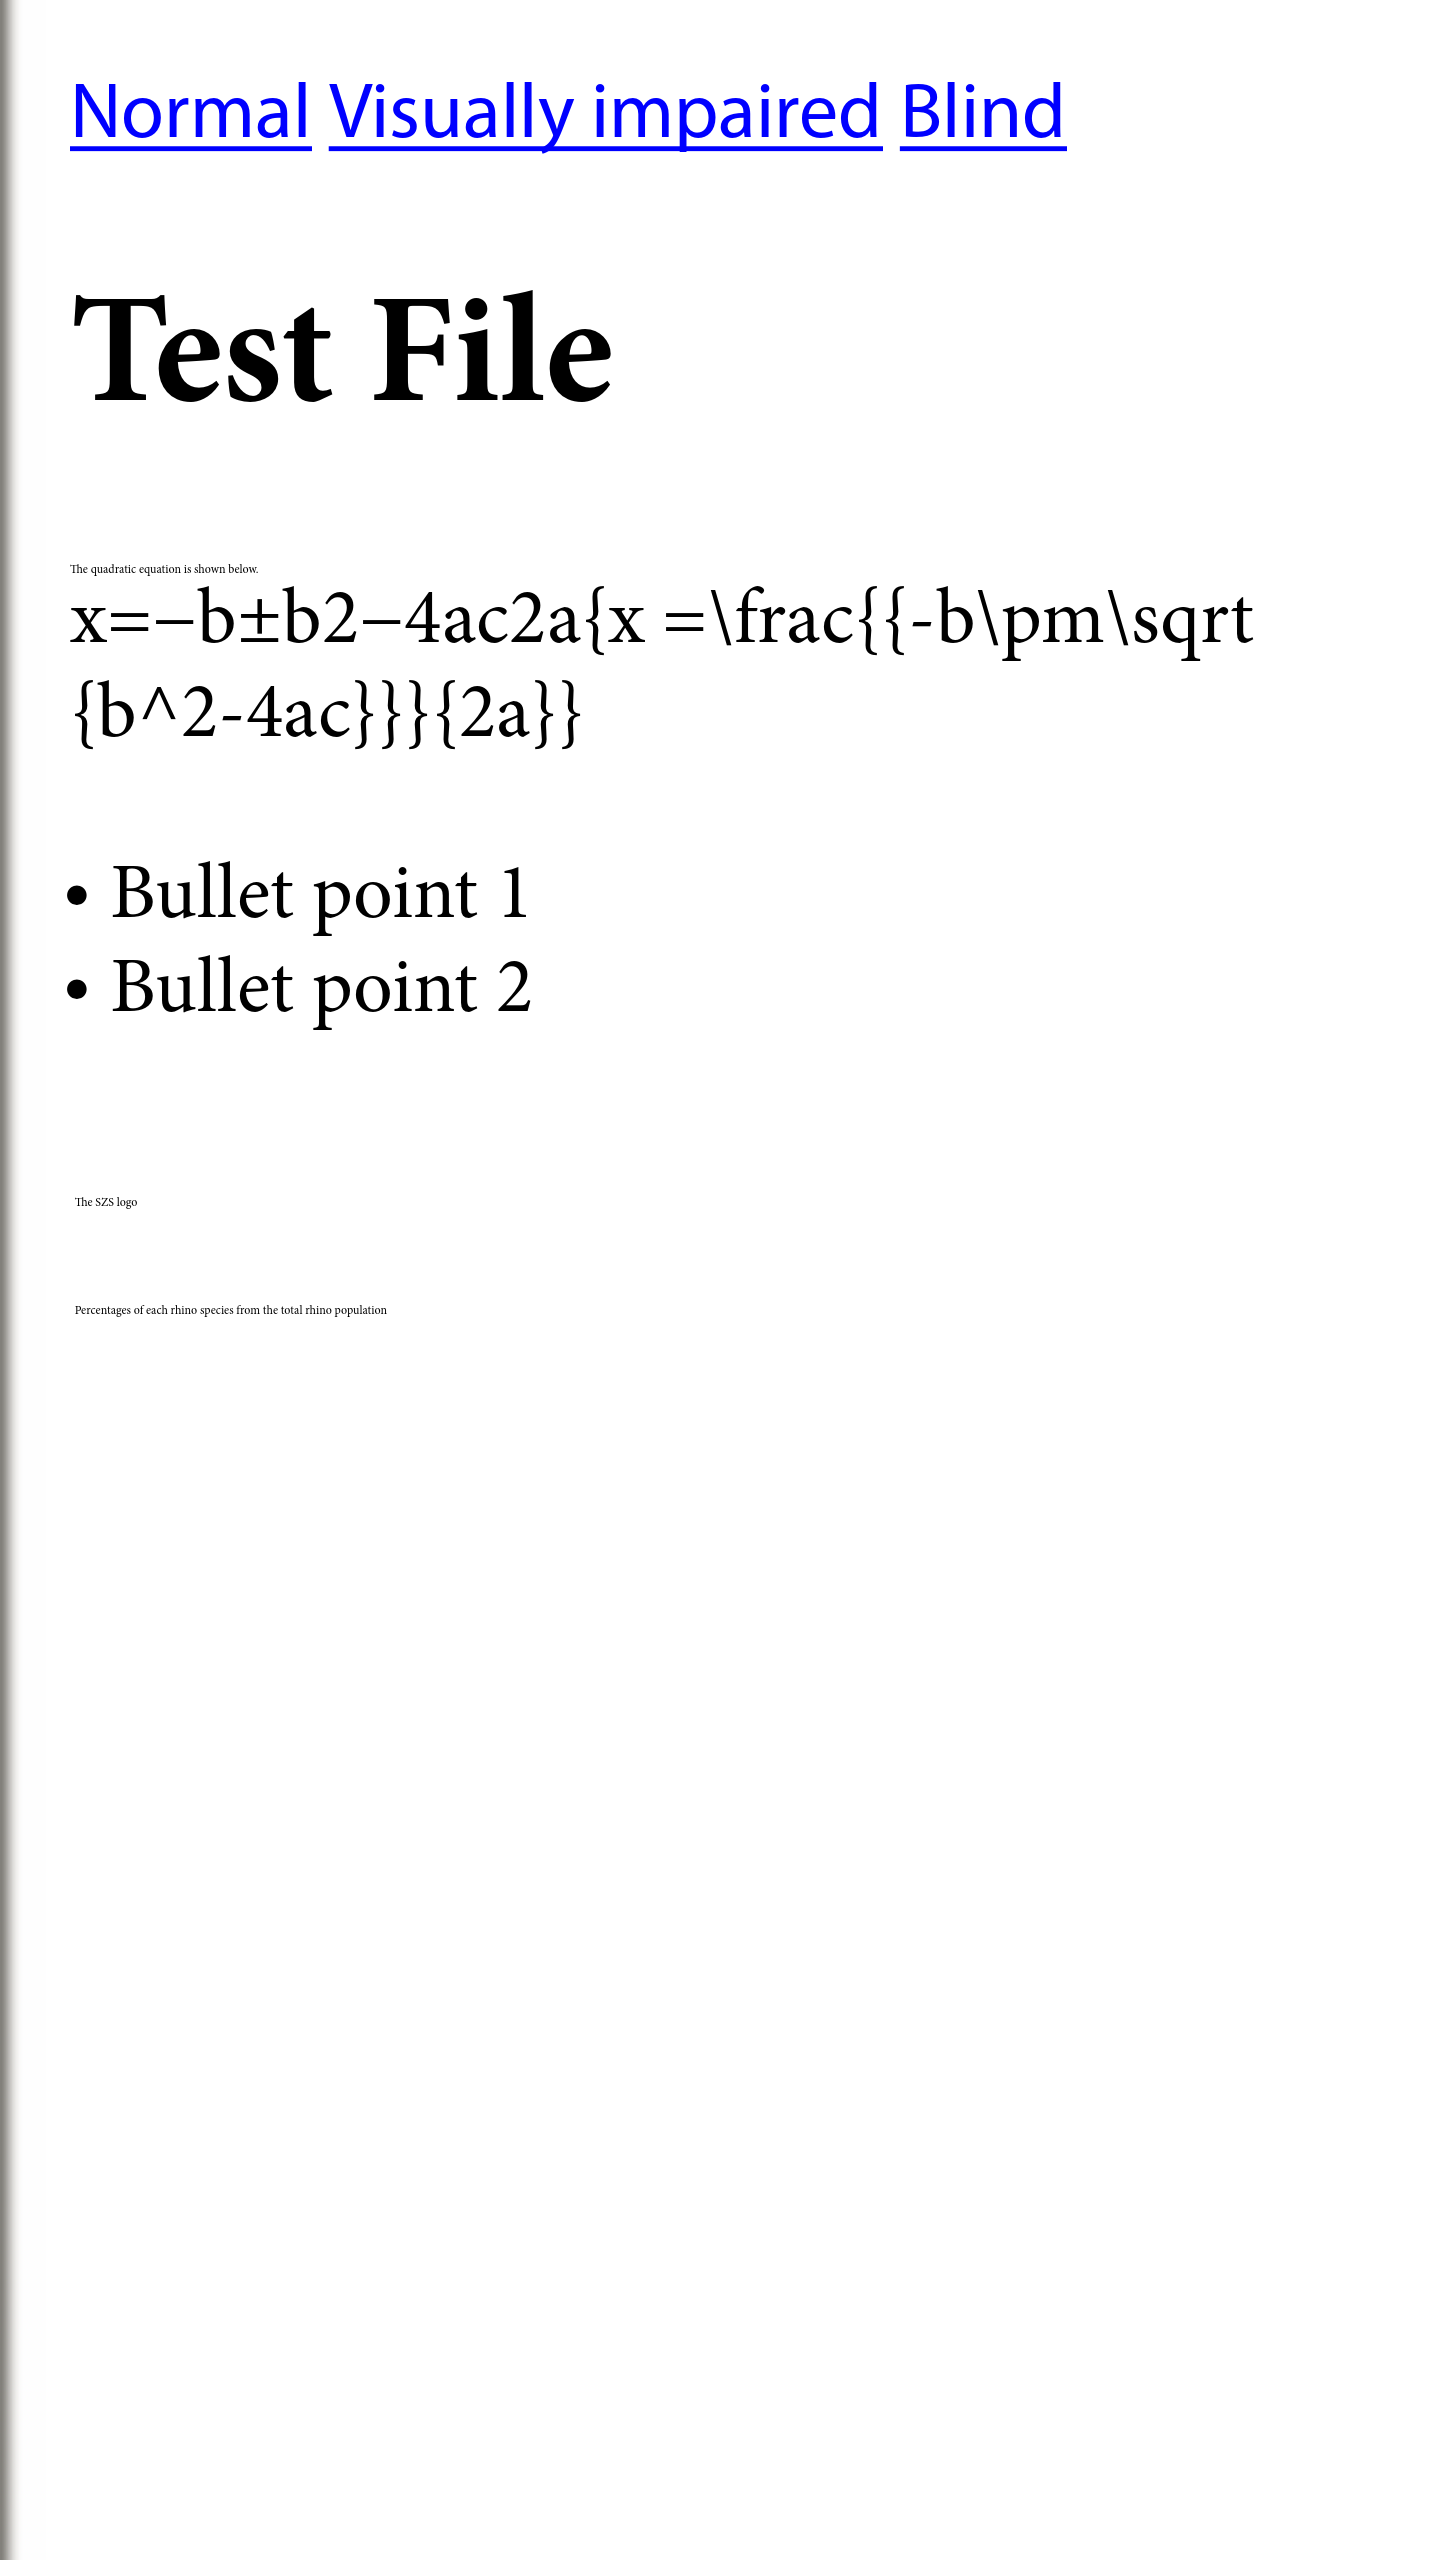
\includegraphics[width=\linewidth/3]{figures/ubreader.png}}
	\caption{The CSS file in UB Reader}
	\label{fig:ubreader}
\end{figure}
UB Reader (Universal Book Reader) is another popular Android E-Book reader\footnote{https://play.google.com/store/apps/details?id=com.mobisystems.ubreader\_west}. The switching mechanism does not work with either standard and as shown in figure \ref{fig:ubreader}, the equation and the images are not shown. Strangely enough, the standard text is shown very small, while links, bullet points and other text is shown much larger.

\section{Reading systems on iOS}
\subsection{Marvin}


Marvin is an app for iOS devices\footnote{https://itunes.apple.com/app/id1086482858} and the JavaScript version is displayed correctly. The CSS version does not work. It also renders the SVG correctly, but it is not in the figure. The only problem is with the script size in the visually impaired display style in \ref{fig:marvinVi}. The exponent of b should be the same size like in Reasily shown in figure \ref{fig:reasilyVi}. This will have to be tested further. The blind display style is shown correctly, much like in figure \ref{fig:reasilyBl}. The iOS screen reader, VoiceOver, works very well in Marvin, identifying all elements correctly.

\begin{figure}[H]
	\centering
	\fbox{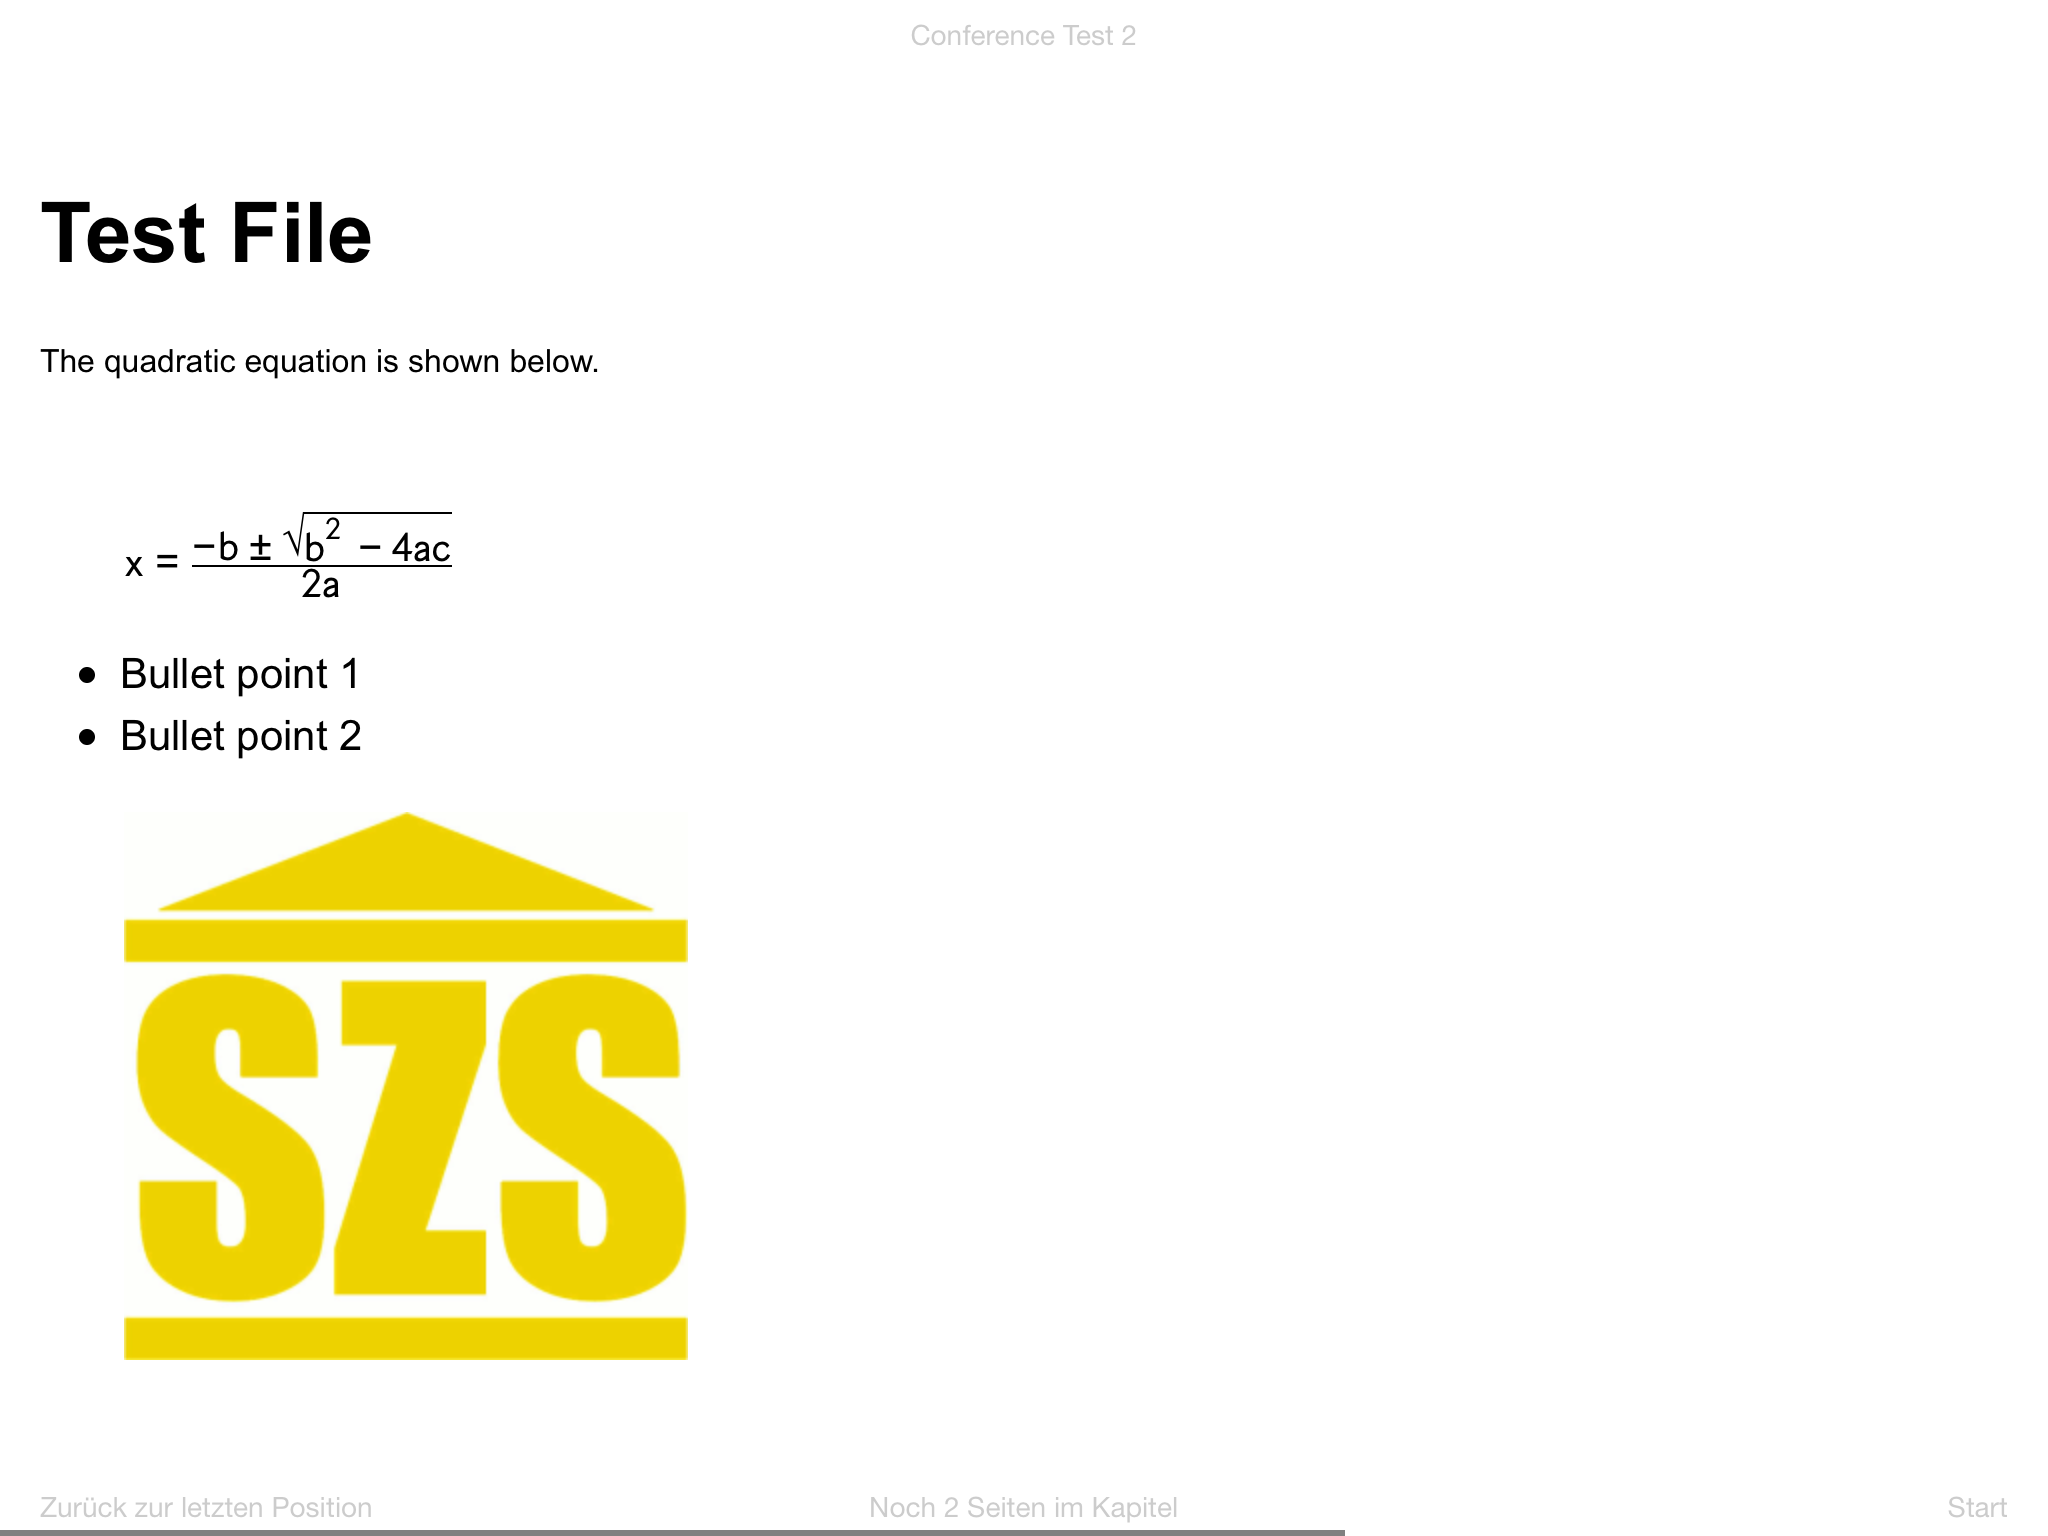
\includegraphics[width=\linewidth*4/5]{figures/MarvinVi.png}}
	\caption{The first half of the visually impaired display style in Marvin}
	\label{fig:marvinVi}
\end{figure}

\begin{comment}
\begin{figure}[H]
	\centering
	\fbox{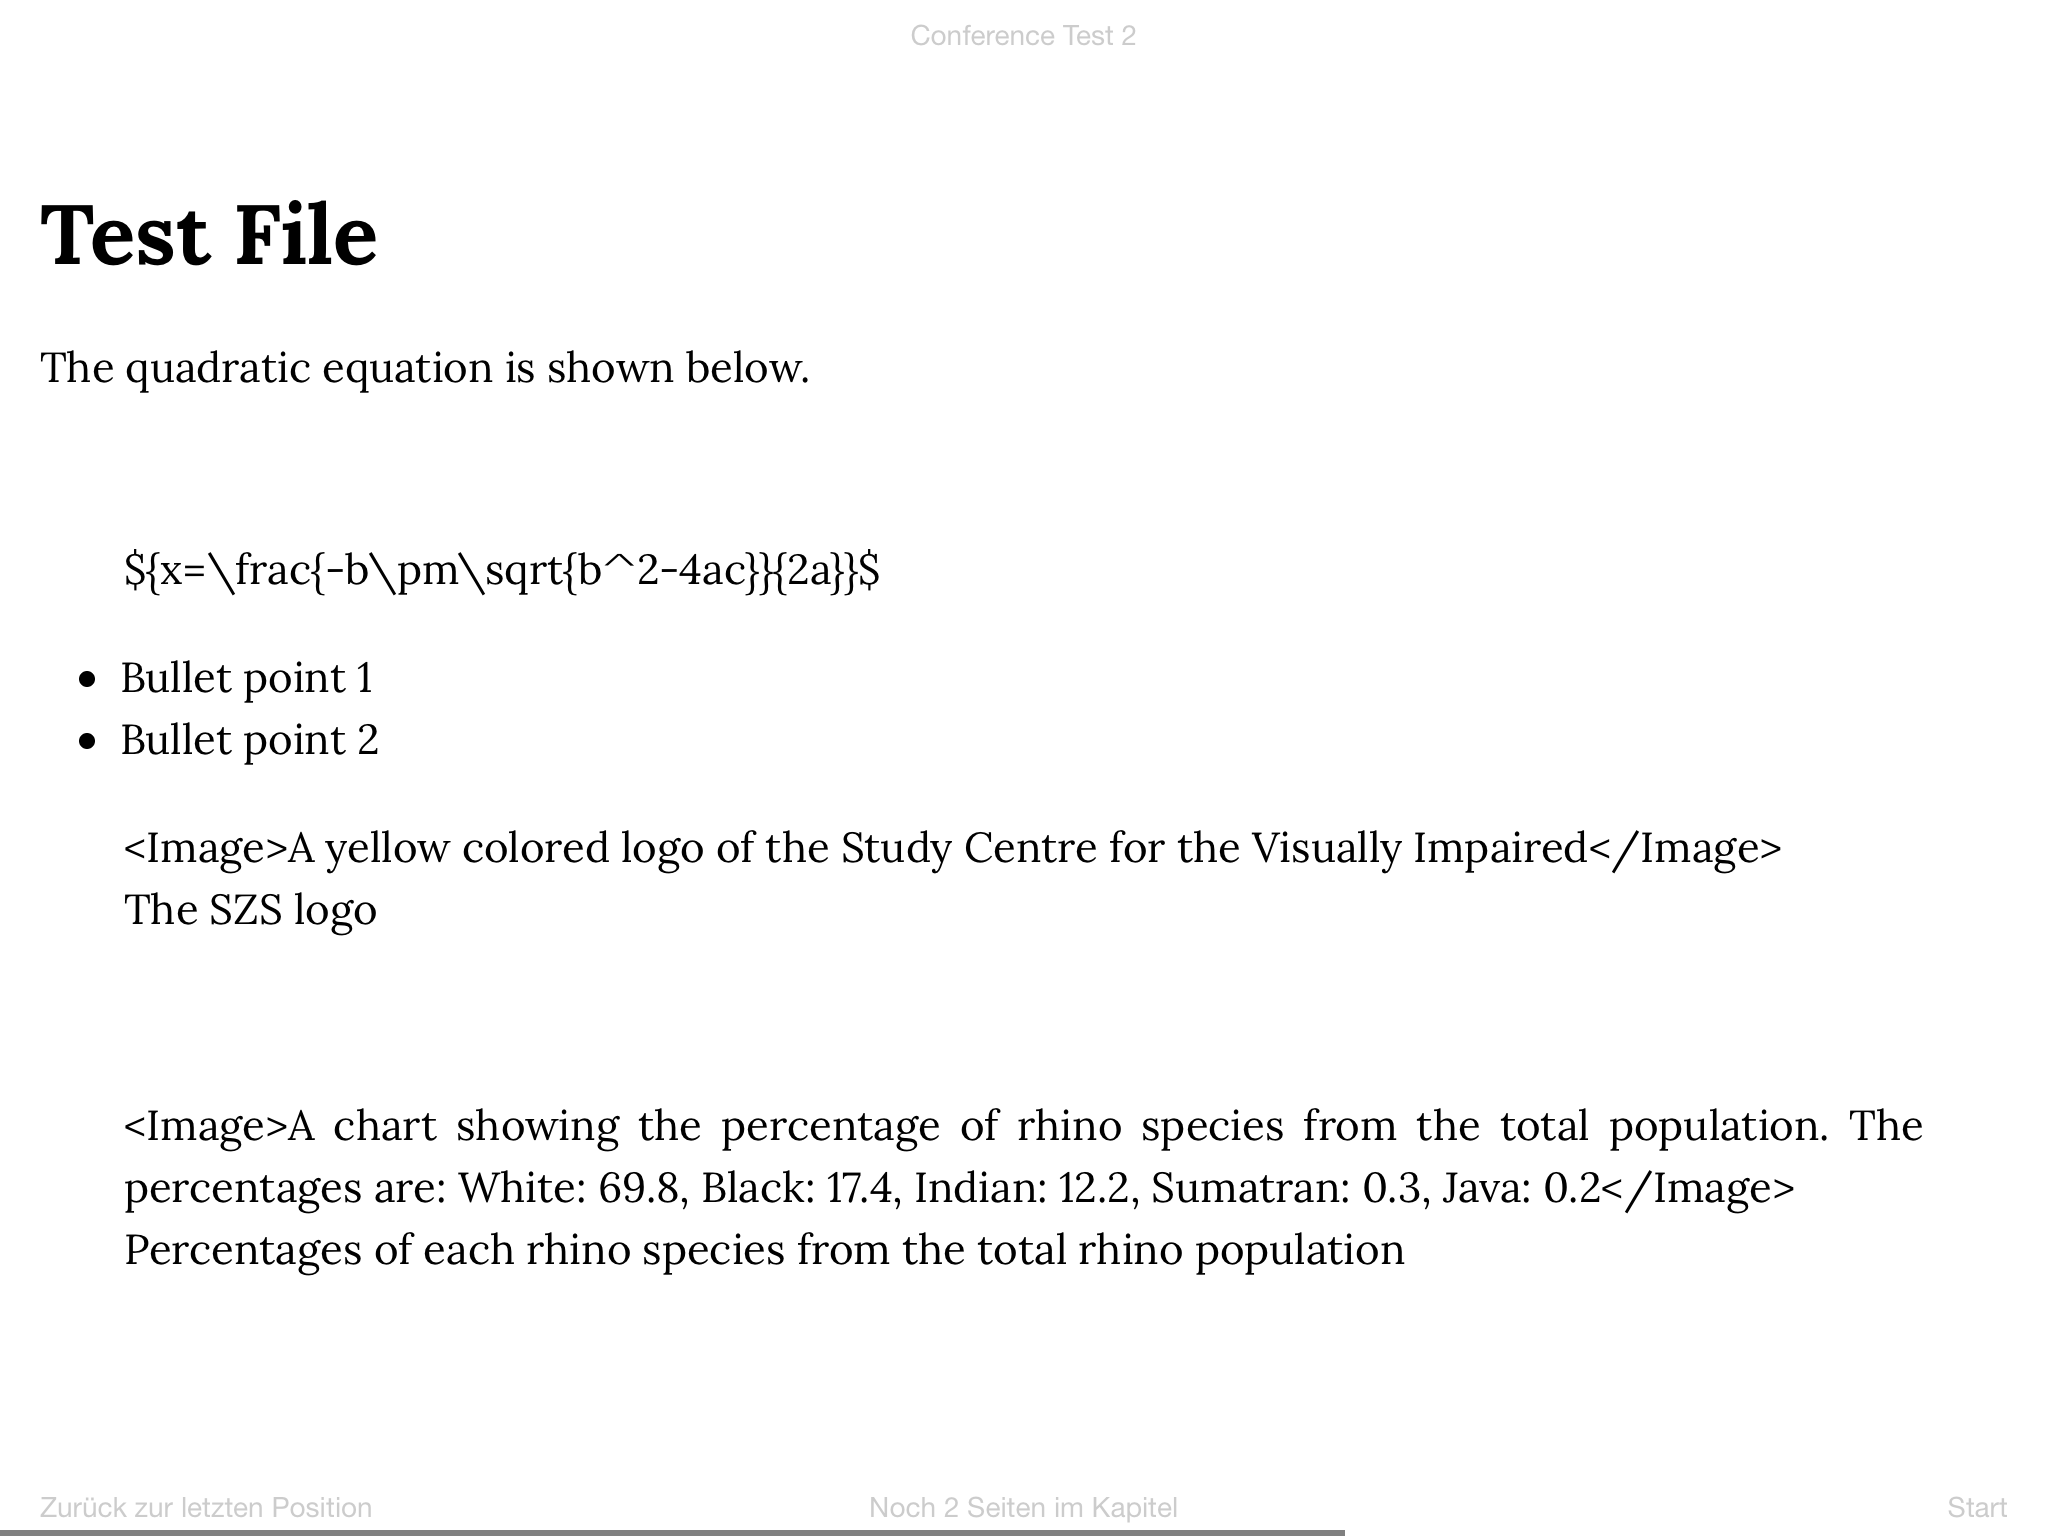
\includegraphics[width=\linewidth*4/5]{figures/MarvinBl.png}}
	\caption{The blind display style in Marvin}
	\label{fig:marvinBl}
\end{figure}
\end{comment}

\subsection{Unusable reading systems}
\subsubsection{iBooks}
iBooks is a E-Book reading system create by Apple for their devices\footnote{https://www.apple.com/ibooks/}. It does not support either one of the switching mechanisms, but can display MathML. Images are not displayed properly, and this likely due to them being in figure elements. The Apple screen reader, VoiceOver, can be used to read EPUB files.

\subsubsection{Yomu}
Yomu EBook Reader on iOS\footnote{https://itunes.apple.com/app/yomu/id562211012} depicts a rendering not seen on other reading systems. In figure \ref{fig:yomu} all elements seem to be displayed correctly. But for some reason the equation appears twice, the first one being a SVG. The SVG is supposed to be hidden and all other reading systems do hide it. It is likely that Yomu does not hide the SVG of an equation which has to included because of the editor in chapter \ref{ch:AccessibleEPUB Editor}. This does not happen to other elements that are hidden the same way. Both the JavaScript and CSS version switching do not work. VoiceOver works with Yomu, and it can identify even individual elements of a SVG, like the percentages shown in the SVG in the test file.
\begin{figure}[H]
	\centering
	\fbox{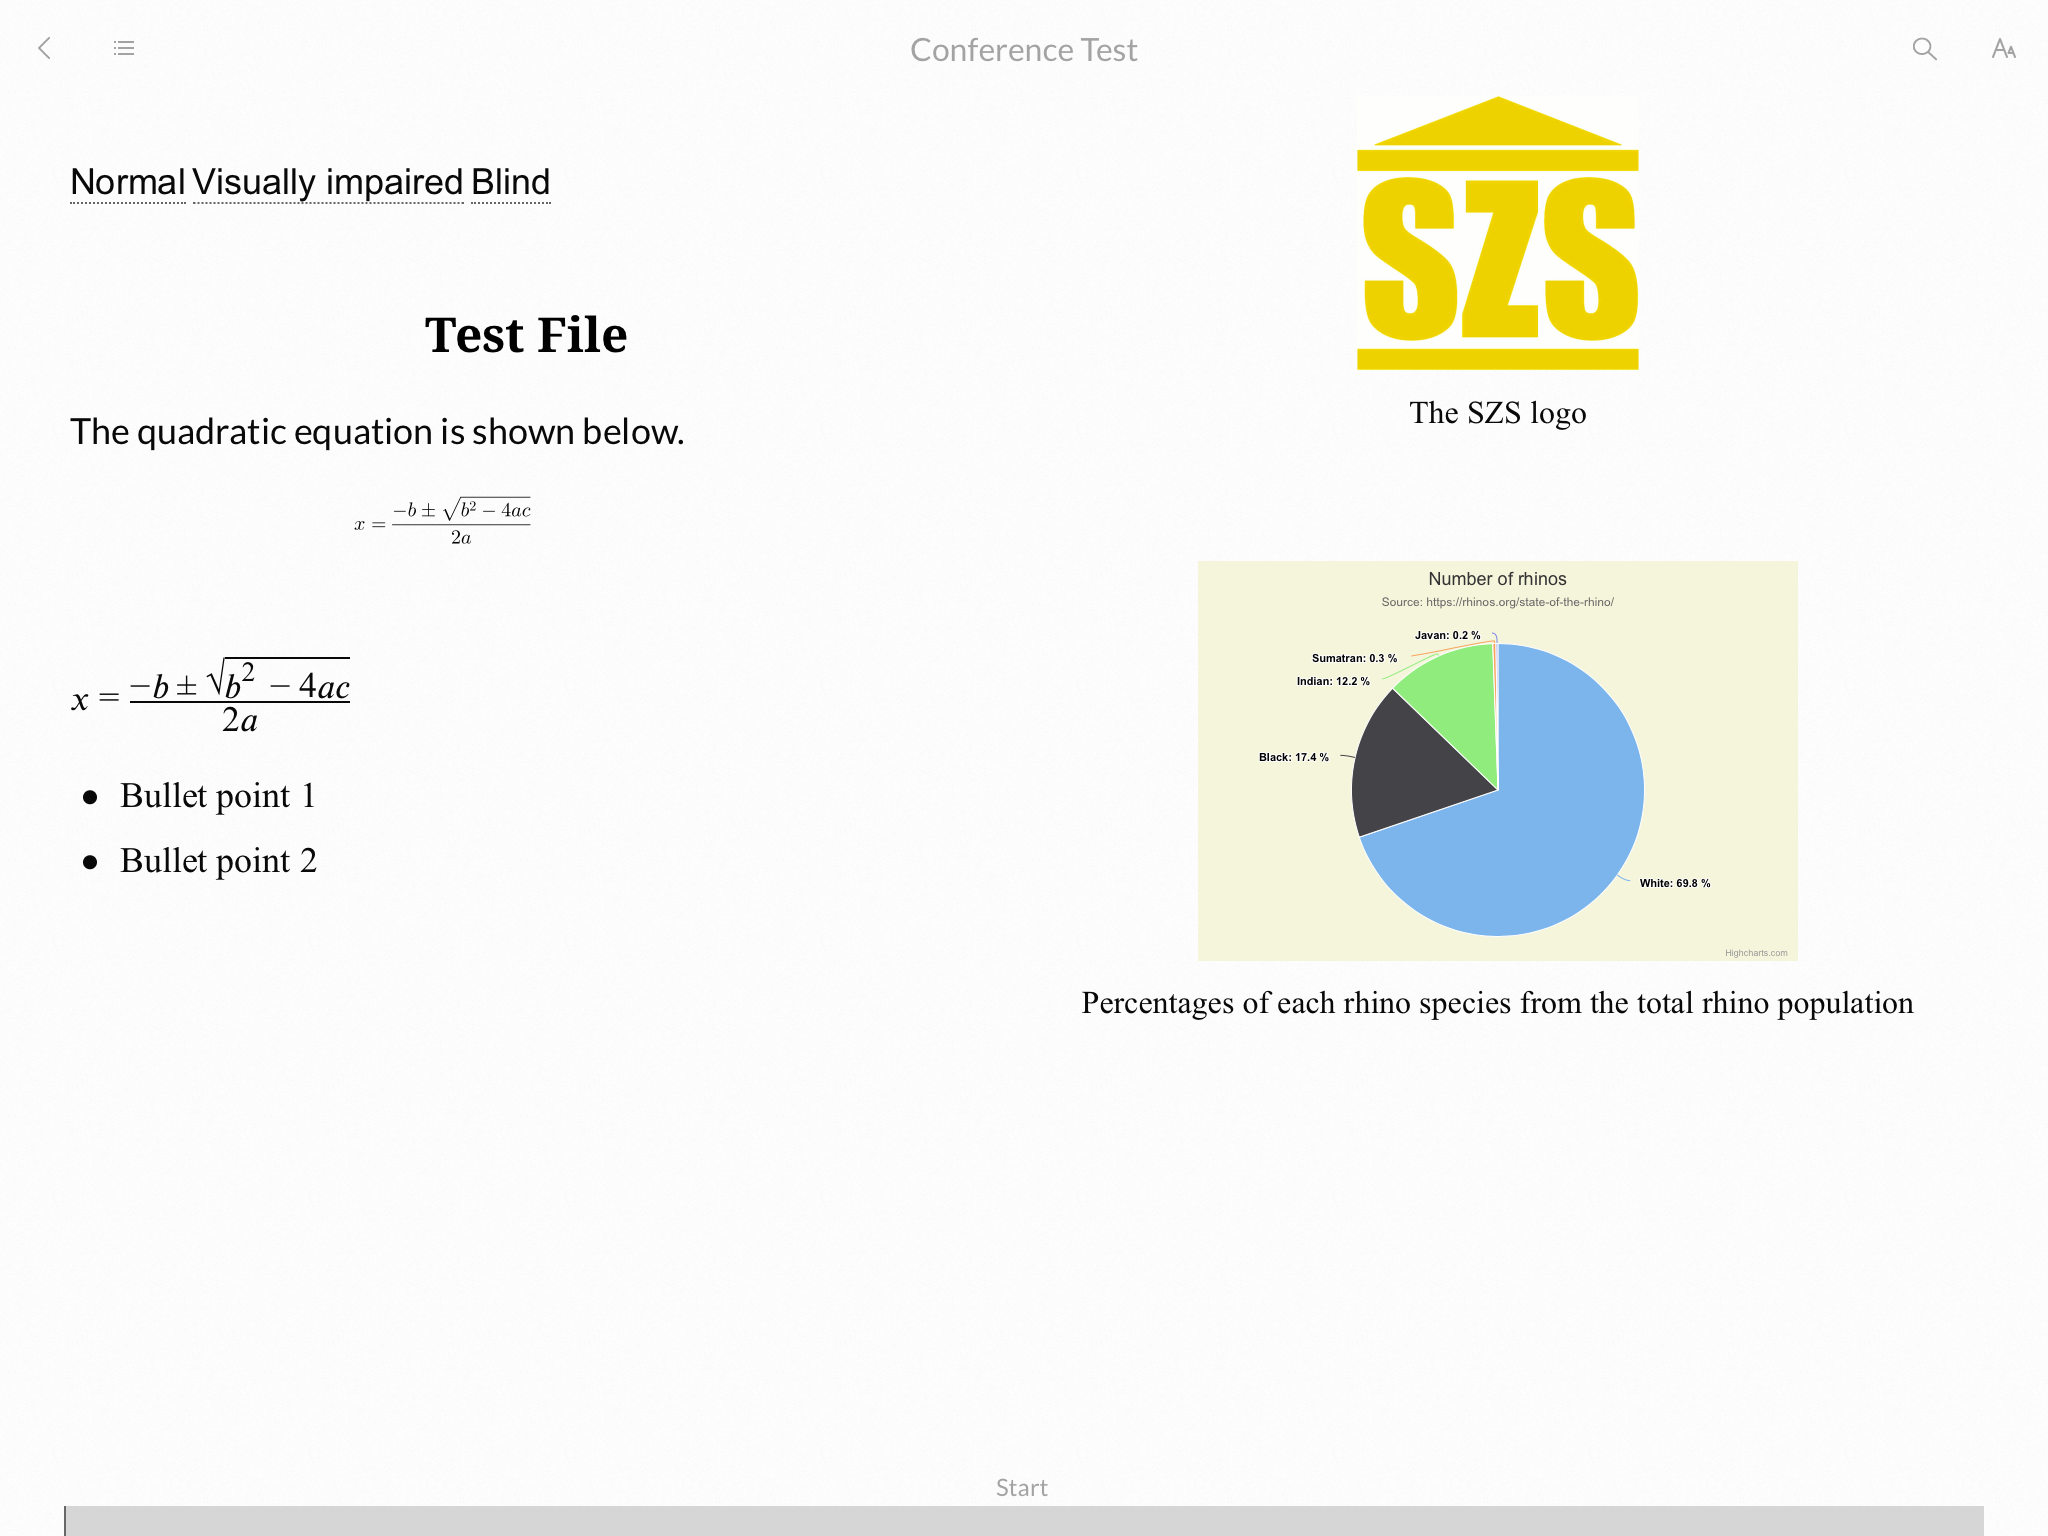
\includegraphics[width=\linewidth*4/5]{figures/Yomu.png}}
	\caption{The CSS file in Yomu}
	\label{fig:yomu}
\end{figure}

\section{Reading systems on Windows}
\subsection{Calibre}
\begin{figure}[H]
	\centering
	\fbox{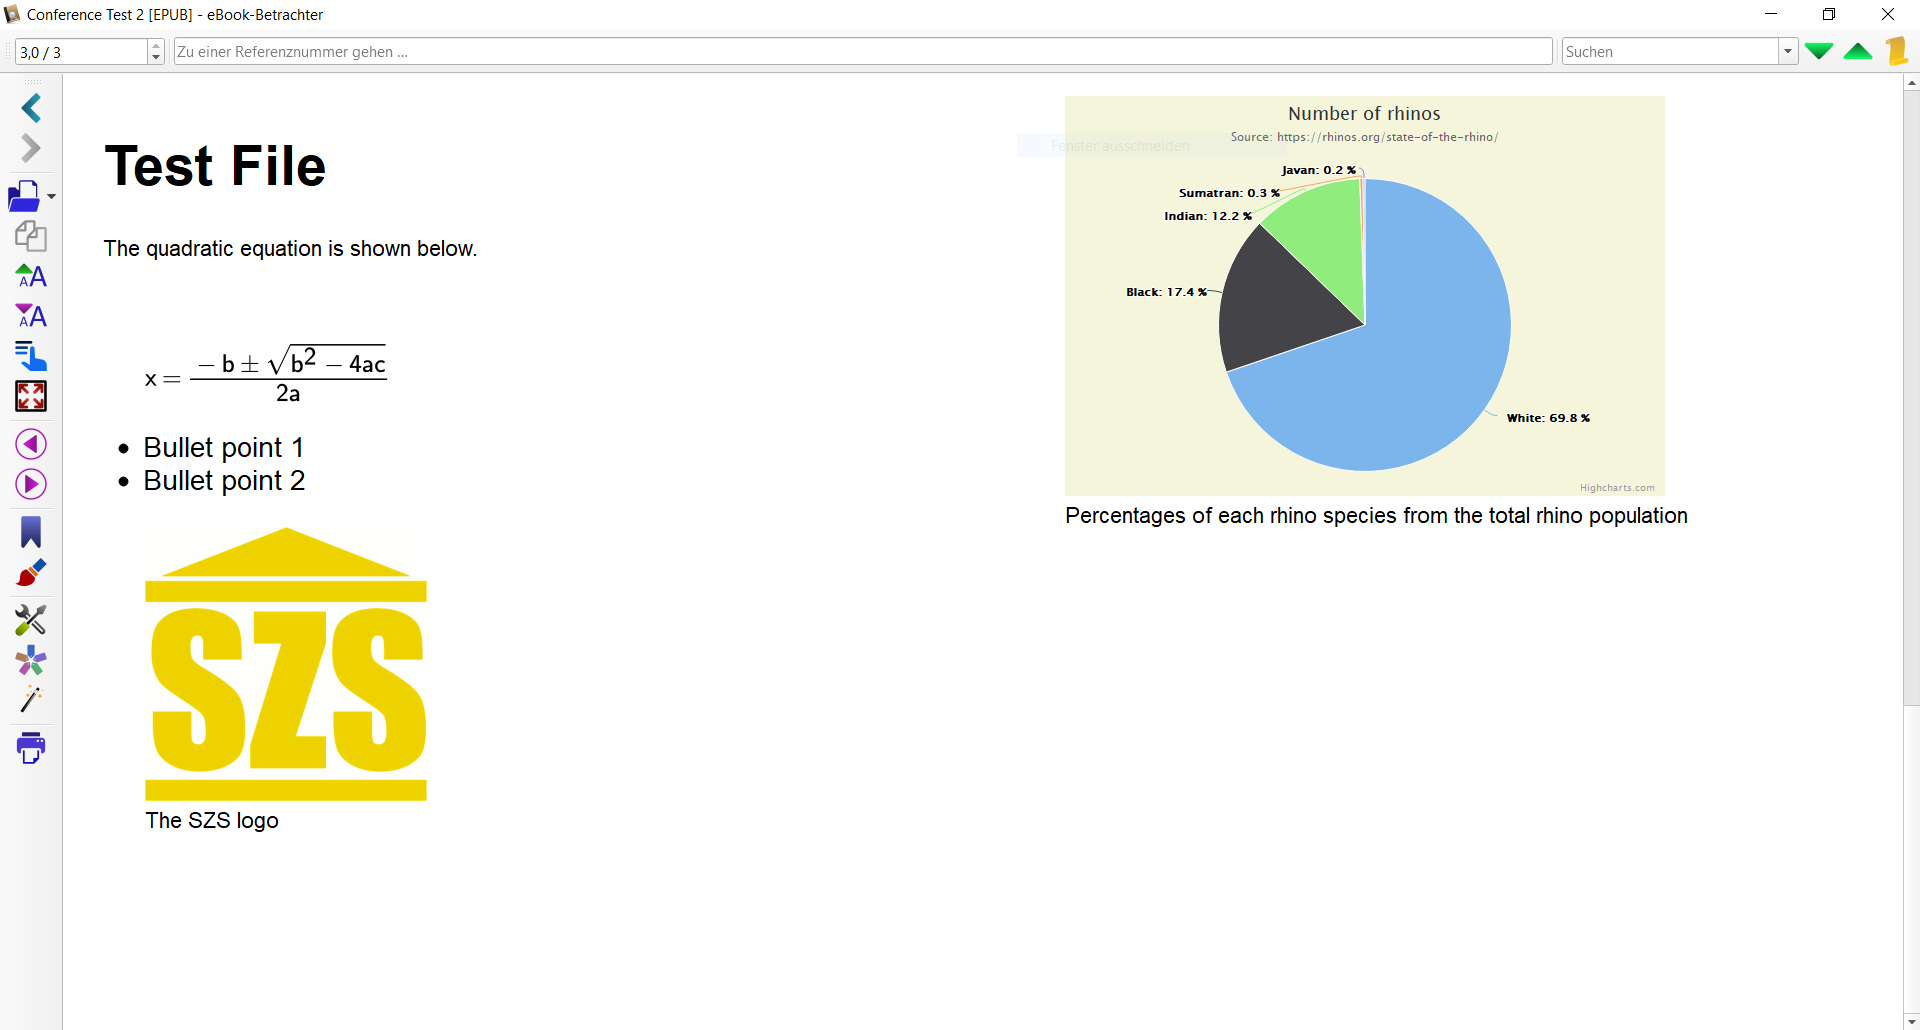
\includegraphics[width=\linewidth]{figures/calibreVi.png}}
	\caption{The visually impaired display style in Calibre}
	\label{fig:calibreVi}
\end{figure}

Calibre is an open source E-Book management system\footnote{https://calibre-ebook.com/}. Calibre is the only reading system to support the JavaScript switching. It has session and not local storage, meaning that the display style is remembered until the EPUB is closed. When it is opened again, it goes back to the default display style. As seen in figure \ref{fig:calibreVi} and \ref{fig:calibreBl}, all elements are shown properly, and when the images are hidden in the blind display style, the alternative text is shown properly. The CSS display style is not supported. One major problem with Calibre is that screen readers are not supported, as it is impossible to access figures and text.

\begin{figure}[H]
	\centering
	\fbox{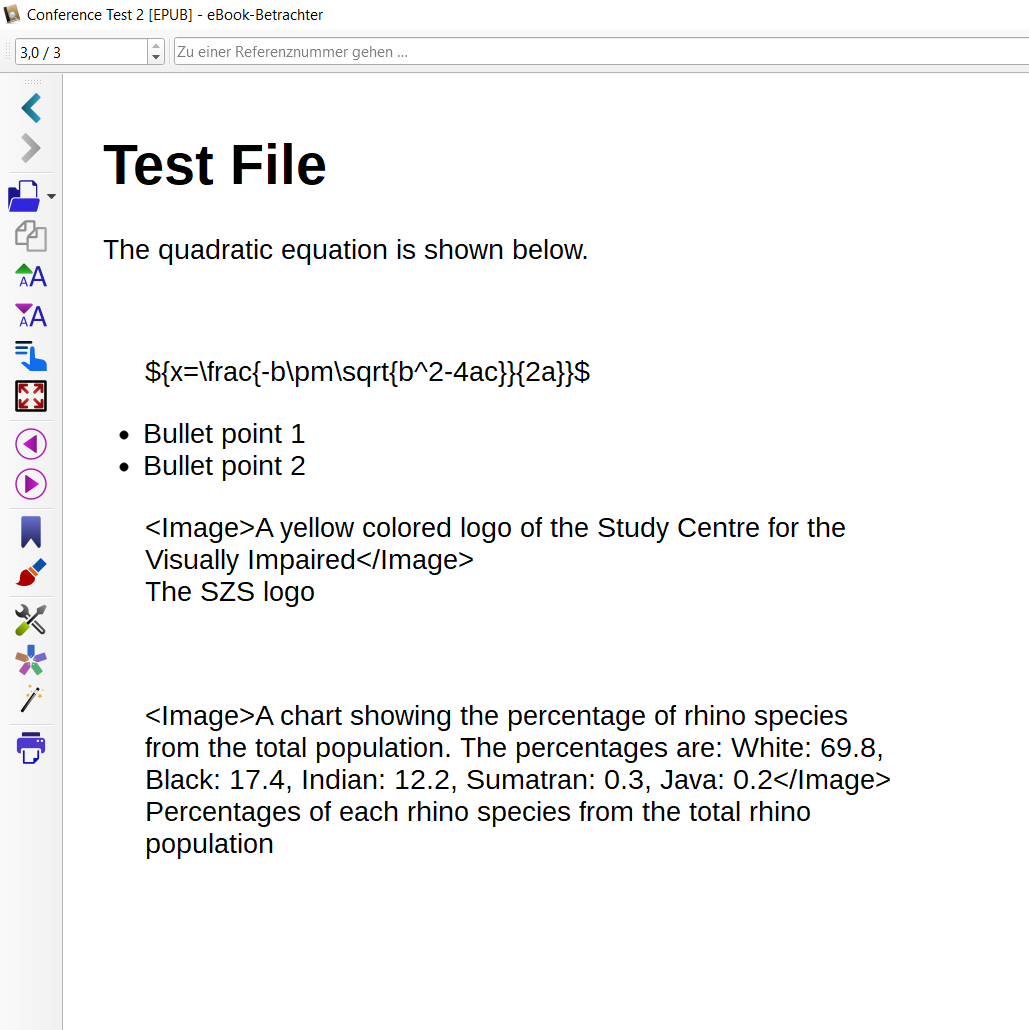
\includegraphics[width=\linewidth*3/5]{figures/calibreBl.png}}
	\caption{The blind display style in Calibre}
	\label{fig:calibreBl}
\end{figure}

\subsection{Readium}

\begin{figure}[H]
	\centering
	\fbox{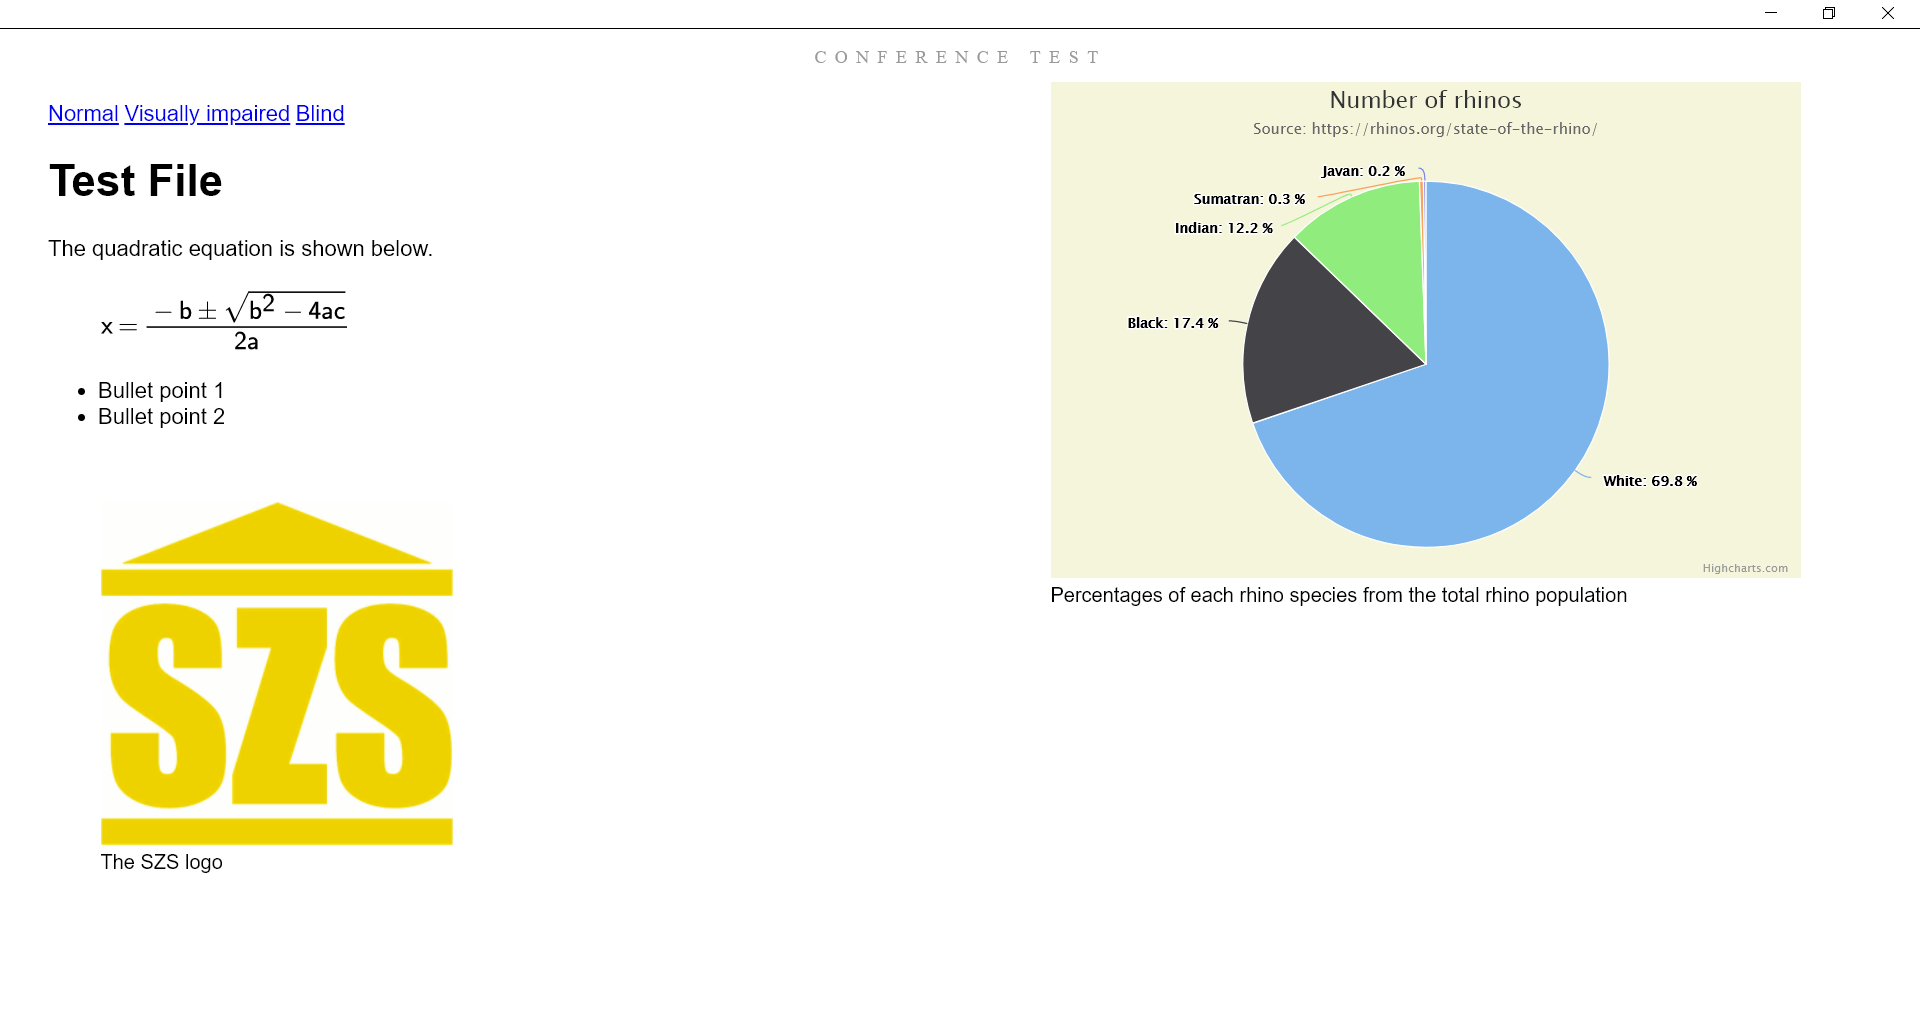
\includegraphics[width=\linewidth]{figures/ReadiumVi.png}}
	\caption{The visually impaired display style in Readium}
	\label{fig:ReadiumVi}
\end{figure}
Readium began as a project of the IDPF as an open source application to create reading systems which follow the newest EPUB standards\footnote{http://readium.org/about/faq}. As such, it supports many of the new features. As shown in figures \ref{fig:ReadiumVi} and \ref{fig:ReadiumBl}, both the visually impaired and blind display style of the CSS standard are shown as intended. The JavaScript standard does not work. It supports screen readers and everything is identified correctly. However, there still is one issue. While testing several CSS EPUB documents, the switching in the short ones did not function properly. In the preview browser in Accessible EPUB and when the individual XHTML files were opened in web browsers, the switching mechanism behaved correctly.


\begin{figure}[H]
	\centering
	\fbox{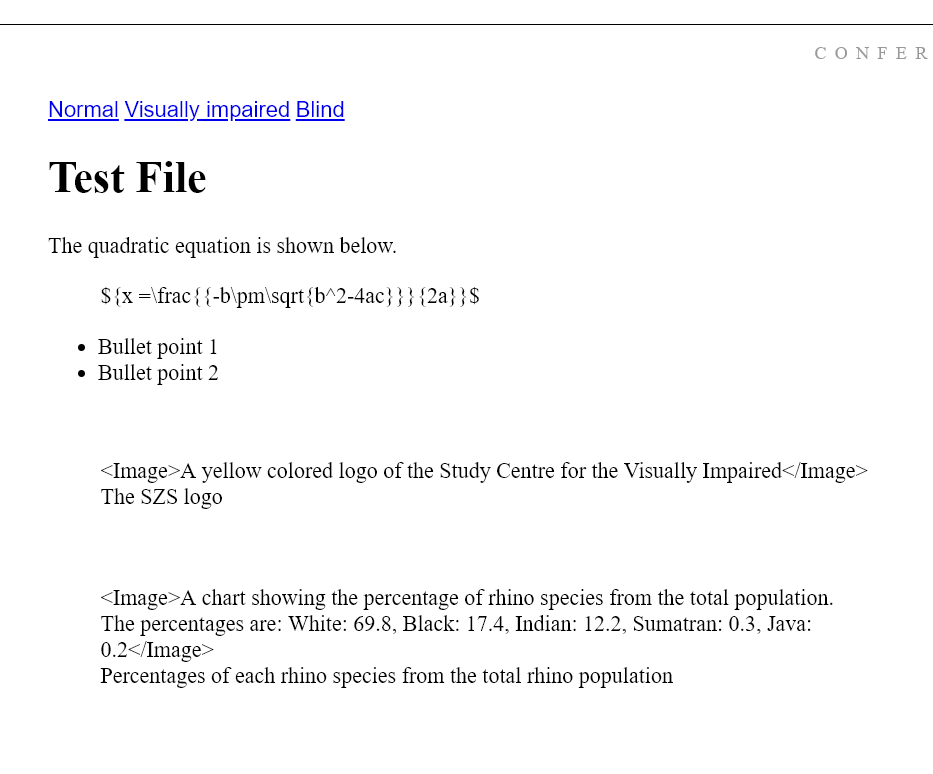
\includegraphics[width=\linewidth]{figures/ReadiumBl.png}}
	\caption{The blind display style in Readium}
	\label{fig:ReadiumBl}
\end{figure}


\subsection{Unusable reading systems}
\subsubsection{Bluefire Reader}
Figure \ref{fig:Bluefire} of the Bluefire Reader\footnote{http://www.bluefirereader.com/bluefire-reader.html} is very similar to figure \ref{fig:tolino} of the Tolino app. They don't show the images and cannot display MathML properly. Both CSS and JavaScript switching do not work. Screen readers can also not read the content of the document.
\begin{figure}[H]
	\centering
	\fbox{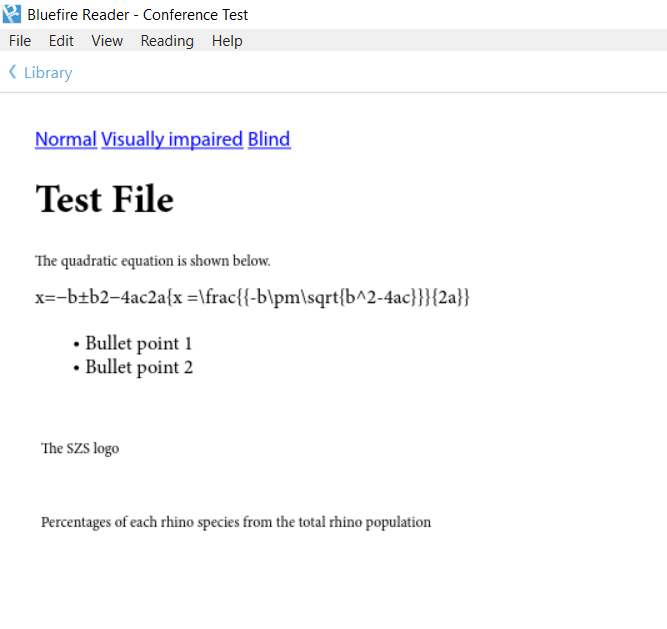
\includegraphics[width=\linewidth*3/5]{figures/Bluefire.png}}
	\caption{The CSS file in Bluefire Reader}
	\label{fig:Bluefire}
\end{figure}
\subsubsection{Icecream Ebook Reader}
Figure \ref{fig:Icecream} shows the CSS test file open in Icecream Ebook Reader\footnote{https://icecreamapps.com/Ebook-Reader/}. While MathML is not displayed properly, the SVG and PNG are shown correctly. The switching mechanism does not work either with CSS or JavaScript and there is no screen reader support.
\begin{figure}[H]
	\centering
	\fbox{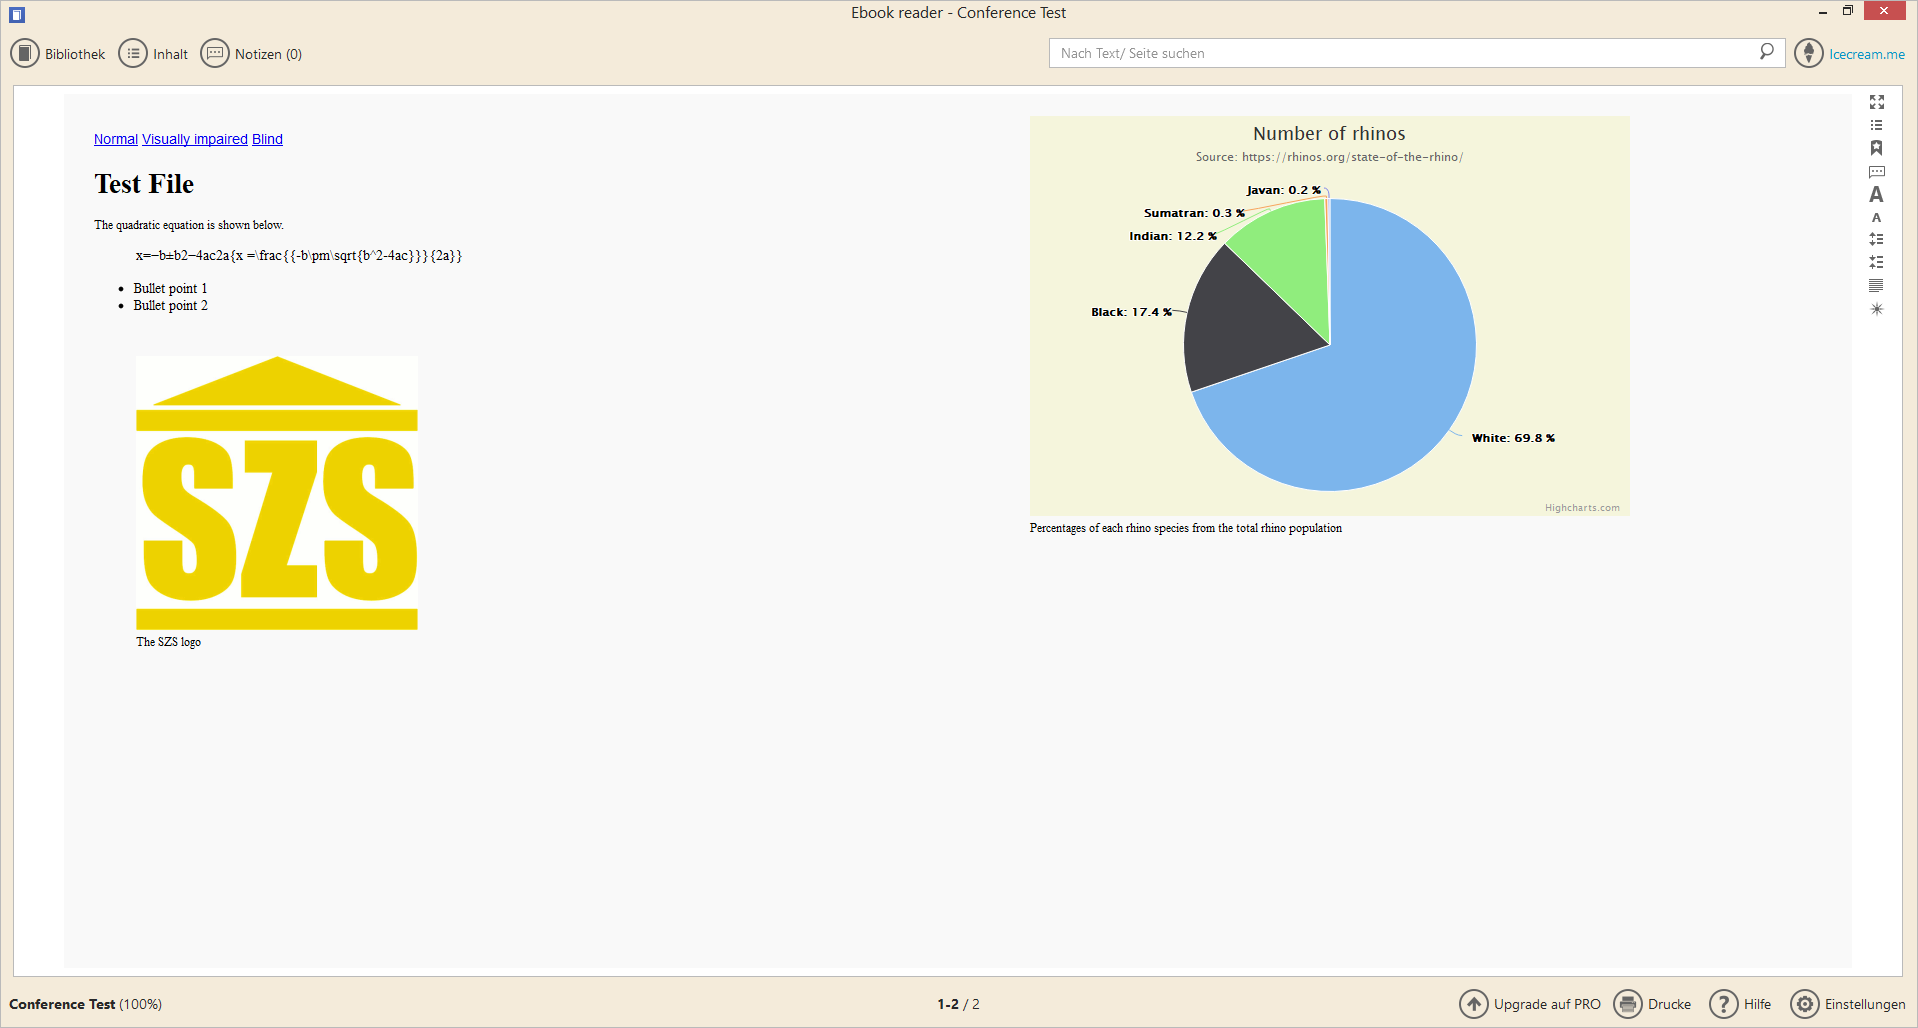
\includegraphics[width=\linewidth]{figures/Icecream.png}}
		\caption{The CSS file in Icecream Ebook Reader}
	\label{fig:Icecream}
\end{figure}

\subsubsection{AZARDI}
AZARDI Desktop\footnote{http://azardi.infogridpacific.com/} is a E-Book reader recommended by the DAISY consortium \cite{daisyAZARDI} as it supports accessibility and it works with the JAWS screen reader. Furthermore, as seen in figure \ref{fig:AZARDI}, it displays most of the content correctly, including MathML. The elements it does not display correctly are the links. They are shown as normal text and it is not indicated that they can be clicked. The switching mechanism does not work in both CSS and JavaScript.
\begin{figure}[H]
	\centering
	\fbox{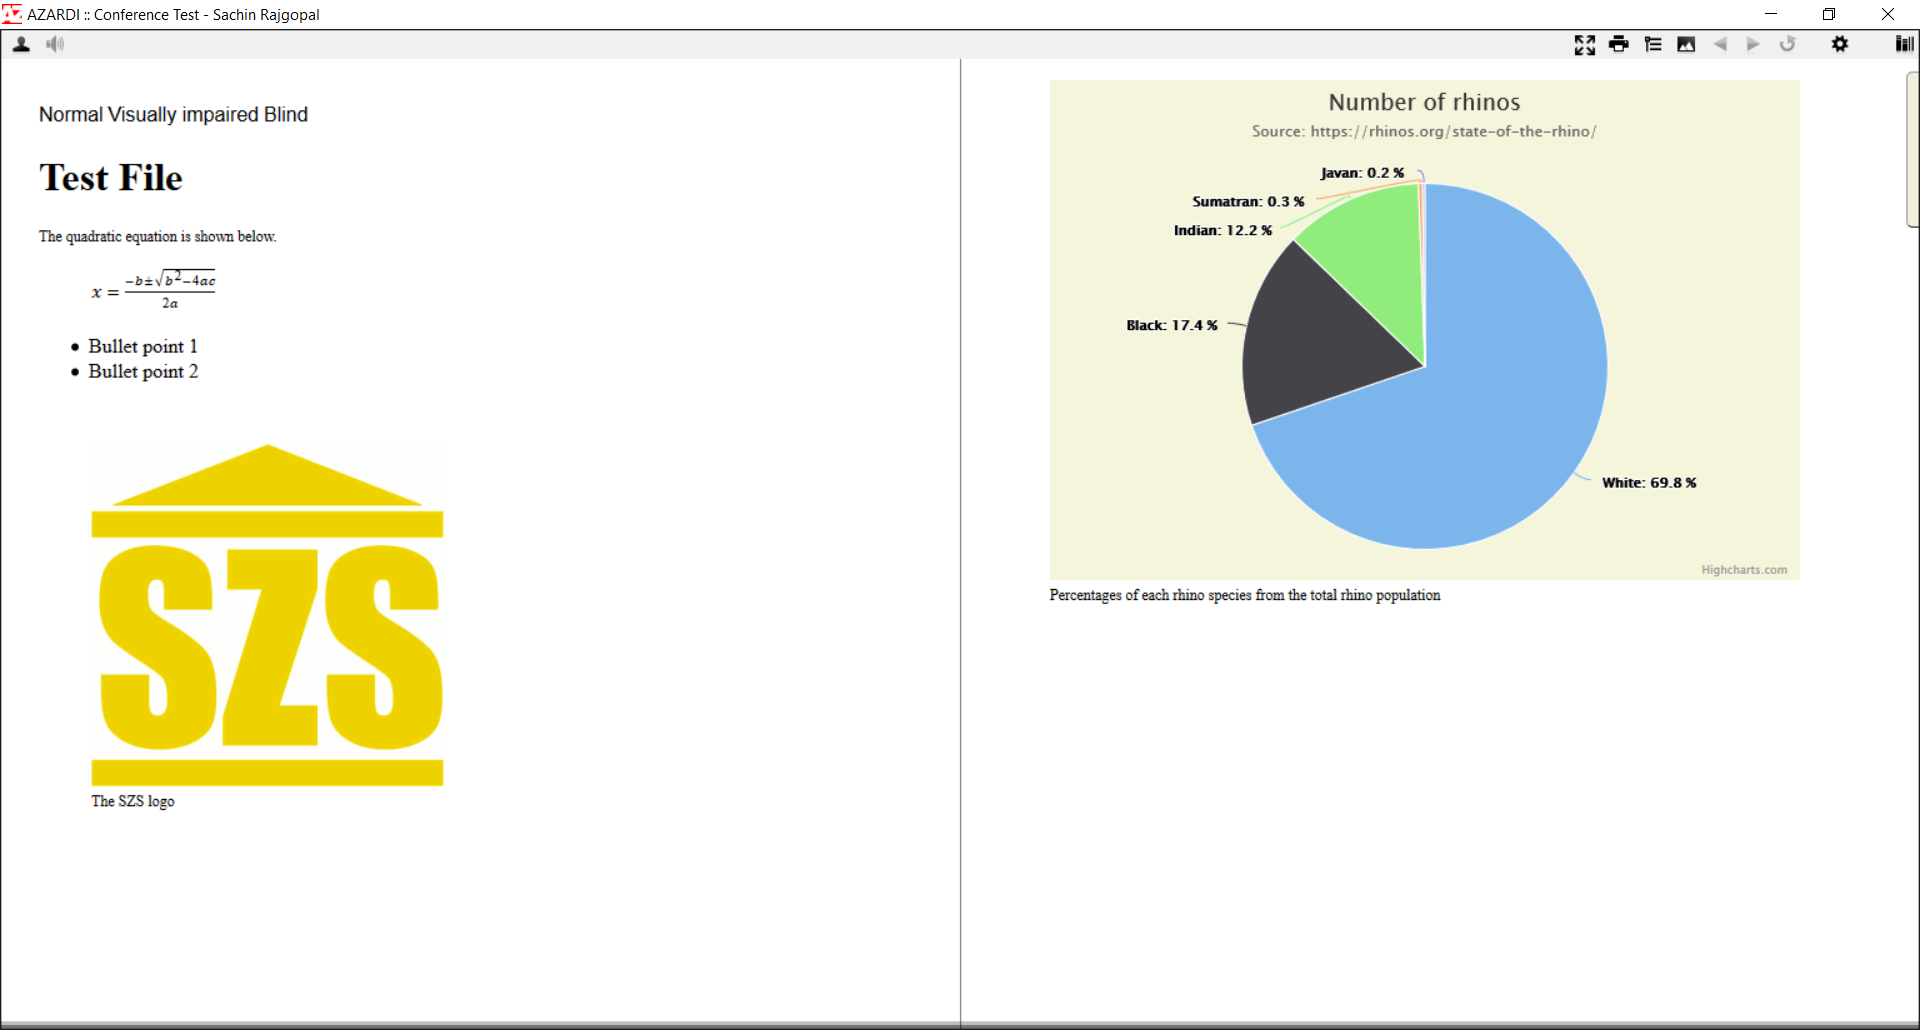
\includegraphics[width=\linewidth]{figures/Azardi.png}}
	\caption{The CSS file in AZARDI}
	\label{fig:AZARDI}
\end{figure}

\subsubsection{Adobe Digital Editions}
\begin{figure}[H]
	\centering
	\fbox{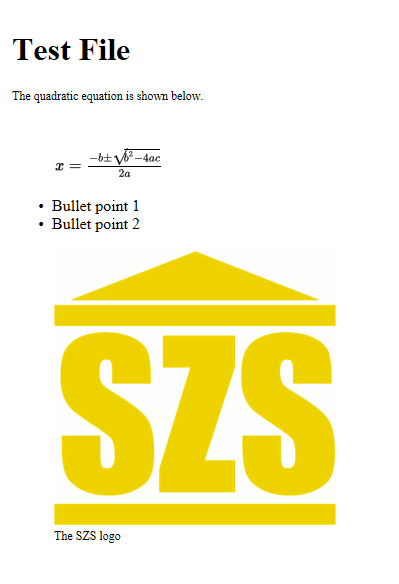
\includegraphics[width=\linewidth/3]{figures/AdobeDigitalEditions.png}}
	\caption{The JavaScript file in Adobe Digital Editions}
	\label{fig:adobeDigital}
\end{figure}

In figure \ref{fig:adobeDigital} the first half of the content in Adobe Digital Editions\footnote{https://www.adobe.com/solutions/ebook/digital-editions.html} is shown. While the equation and the images were displayed correctly, the equation has not been rendered well. The root symbol is poorly formatted and it is not properly spaced. Screen readers do not work.

\section{Discussion: what do developers have to do?}

The EPUB 3 specification \cite{EPUBspecs} was recommended on the 11th of October 2011. More than 6 years later, most of the EPUB reading systems do not support the new features, such as MathML and CSS 3. Developers have to start supporting the new features as soon as possible. The CSS standard only works in Reasily and Readium, while the JavaScript standard  works in Marvin and Calibre. JavaScript is optional so developers don't have to necessarily support that standard, but CSS is part of the EPUB specification. It is important that the new CSS features will be supported soon, so that the CSS standard functions properly. Even Readium which was originally created by the IDPF does not support the CSS perfectly. It seems like EPUB 3 will remain the standard for a longer period of time as EPUB 3.1 specification was just recommended on the 5th of January 2017 and it was just a small update. So developers of EPUB reading systems can be assured that the EPUB 3 specification won't be completely overworked in the foreseeable future and have some security for the future. 

\section{Conclusion}
\begin{table}
	\centering
	\caption{Features supported by several EPUB reading systems}
	\begin{tabular}{| c | c | c | c | c |}
		\hline
		& CSS & JavaScript & MathML & Screen reader \\ \hline
		\textbf{Reasily} & \cmark & \xmark & \cmark & \cmark \\  \hline
		Tolino & \xmark & \xmark & \xmark & \xmark \\ \hline
		Gitden & \xmark & \xmark & \cmark & \cmark \\ \hline
		FBReader & \xmark & \xmark & \xmark & \xmark \\ \hline
		UB Reader & \xmark & \xmark & \xmark & \xmark \\ \hline
		
		\textbf{Marvin} & \xmark & \cmark & \cmark & \cmark \\ \hline
		iBooks & \xmark & \xmark & \cmark & \cmark \\ \hline
		Yomu & \xmark & \xmark & \cmark & \cmark \\ \hline
		
		\textbf{Calibre} & \xmark & \cmark & \cmark & \xmark \\ \hline
		\textbf{Readium} & \cmark & \xmark & \cmark & \cmark \\ \hline		
		Bluefire Reader & \xmark & \xmark & \xmark & \xmark \\ \hline
		Icecream Ebook Reader & \xmark & \xmark & \xmark & \xmark \\ \hline
		AZARDI & \xmark & \xmark & \cmark & \cmark \\ \hline		
		Adobe Digital Editions & \xmark & \xmark & \cmark & \cmark \\ \hline
		
	\end{tabular}
	\label{fig:table}
\end{table}

As seen figure \ref{fig:table}, many EPUB reading systems do not even process MathML correctly, and many were chosen in this thesis due to them listing MathML support as a feature. Even fewer can use the switching mechanism with either version. A few of them do work though. On Android Reasily is the recommended app as it works well with the CSS version. Marvin can display with JavaScript version correctly in iOS. On Windows 10 Calibre works the best with the JavaScript version, but screen readers do not identify the content area. Readium works well with CSS version, but there are still some usability issues where short files do not switch display styles. It is, however, still the best option on Windows as it screen readers can work with it.
\chapter{AccessibleEPUB Editor}
\label{ch:AccessibleEPUB Editor}

The AccessibleEPUB editor will be presented with each Windows form covering a separate section.

\section{Requirements}

There are a variety of requirements which have to be fulfilled the editor. Most importantly, it has easy to use and not require any programming knowledge to use, except for LaTeX code for equations. If no equations are needed in the document, then there must be programming ability asked of the user. 

\section{Programming language}

The first question was in which programming language should the editor be implemented in. C\# and Java were picked early as the two main options, as both of them are object oriented and natively support forms. Furthermore, both support the ability to make the programs themselves accessible for blind users. C\# has several accessibility properties, like AccessibilityDescription and AccessibilityName, which are passed to the screen reader. Java uses the Java Accessibility Bridge which makes it accessible to screen readers. Java is platform independent, and while C\# programs can run on Mac OS and Linux, it relies heavily on Windows and its features. However, Java is not already installed on any operating system, while C\# programs can run on Windows machine with only .NET as prerequisite. The target .NET version of the editor is contained in Windows 10. Therefore the editor was programmed in C\#, as the users were predominantly Windows users and don't have to install prerequisites.

\section{Main window with editor and preview}

\subsubsection{HTML Editor}

\begin{figure}
	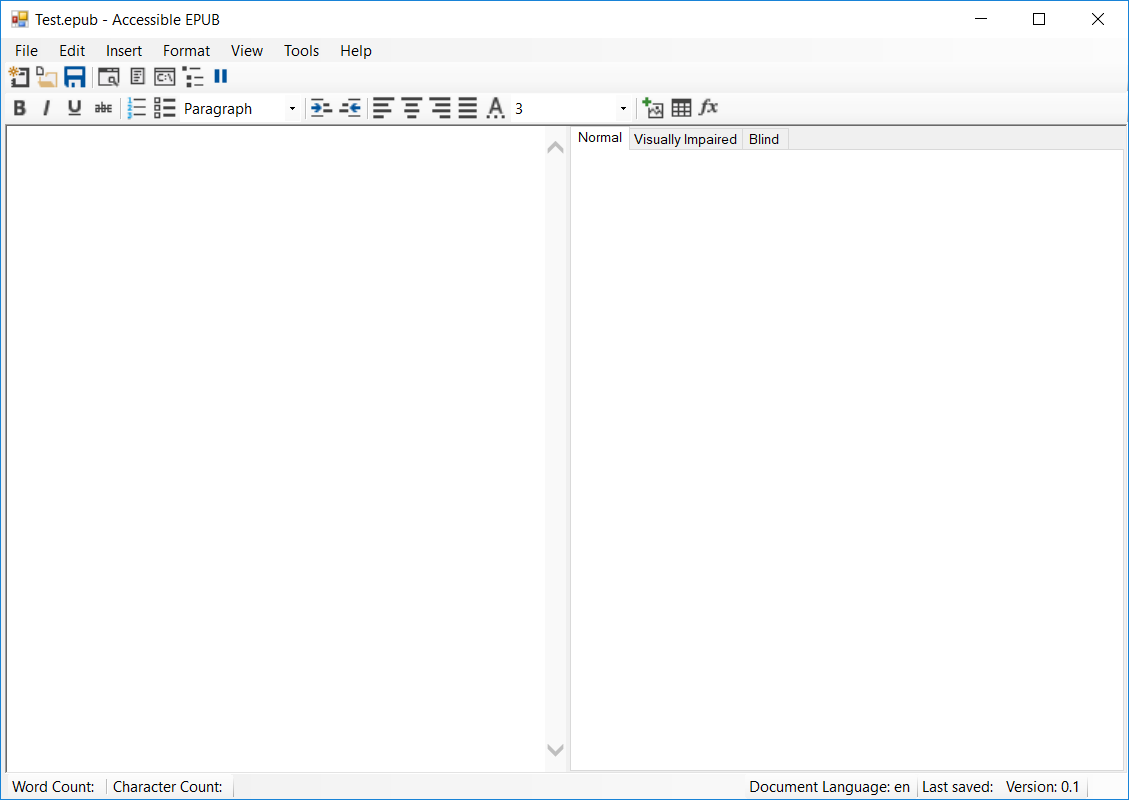
\includegraphics[width=\linewidth]{figures/formJs.png}	
	\caption{Main window with HTML editor and JavaScript switching preview}
	\label{fig:formJs}
\end{figure}

The main window required the most programming and therefore also had its fair share of problems. The first issue was regarding the editor on the left hand side in figure \ref{fig:formJs}. At first a What-You-See-Is-What-You-Get(WYSIWYG) HTML editor was not intended, as it hides semantic information about the EPUB. The initial approach involved editing semantic information of XHTML elements, like images, and changing things like the src, alt, etc. This was still in the early, rough stages and the approach seemed too complicated, so the WYSIWYG editor was chosen instead. 

The second issue was how to implement the WYSIWYG HTML editor. Programming it from scratch would not be possible in the time allocated to a bachelor thesis, as it would involve creating a browser engine. Fortunately, the inbuilt browser in C\#, WebBrowser, allows editing with just a few lines of code. The WebBrowser control is based on Internet Explorer and displays web pages like it. It uses Internet Explorer version 6 as default, which does not display certain CSS properties such as \lstinline|max-width| and cannot display SVGs. To fix this issue, some code has to be run when the form has loaded which determines the Internet Explorer version on the computer and loads the newest one to the HTML editor. After this SVGs and the CSS properties functioned as desired. 

A major issue with the HTML editor is that content written in it is in HTML, while EPUB requires XHTML. While there aren't major differences, there are some small ones such as independent tags like \lstinline|<br>| have to be self closing and written as \lstinline|<br/>| in XHTML. If this is not done the EPUB reader will specify an error. Therefore a tool has to convert the HTML code to XHTML. There are several packages available, one of them being HtmlAgilityPack\footnote{http://html-agility-pack.net/}. It can convert HTML and XHTML and also correct HTML parsing errors such as not closed tags. HtmlAgilityPack functioned well and as expected at first. The resulting code was in XHTML. However, there soon was an error. Many Greek signs, such as the sign "$\wedge$", were displayed as question mark. This meant HtmlAgilityPack could not be used. 

Another available package was TidyManaged\footnote{https://github.com/markbeaton/TidyManaged}, was also used, but it did not convert the code properly to XHTMl. The third attempt involved using SgmlReader\footnote{https://github.com/lovettchris/SgmlReader}, which converts SGML content, like HTML, to XML content, like XHTML. It successfully parsed the HTML and was able to convert mathematical signs properly. It did not create a XML declaration at the top of the document, but this was simpler to solve. A standard XML declaration was just added to the document and the new XHTML document was properly rendered by the browser.


\begin{figure}
	\begin{center}
		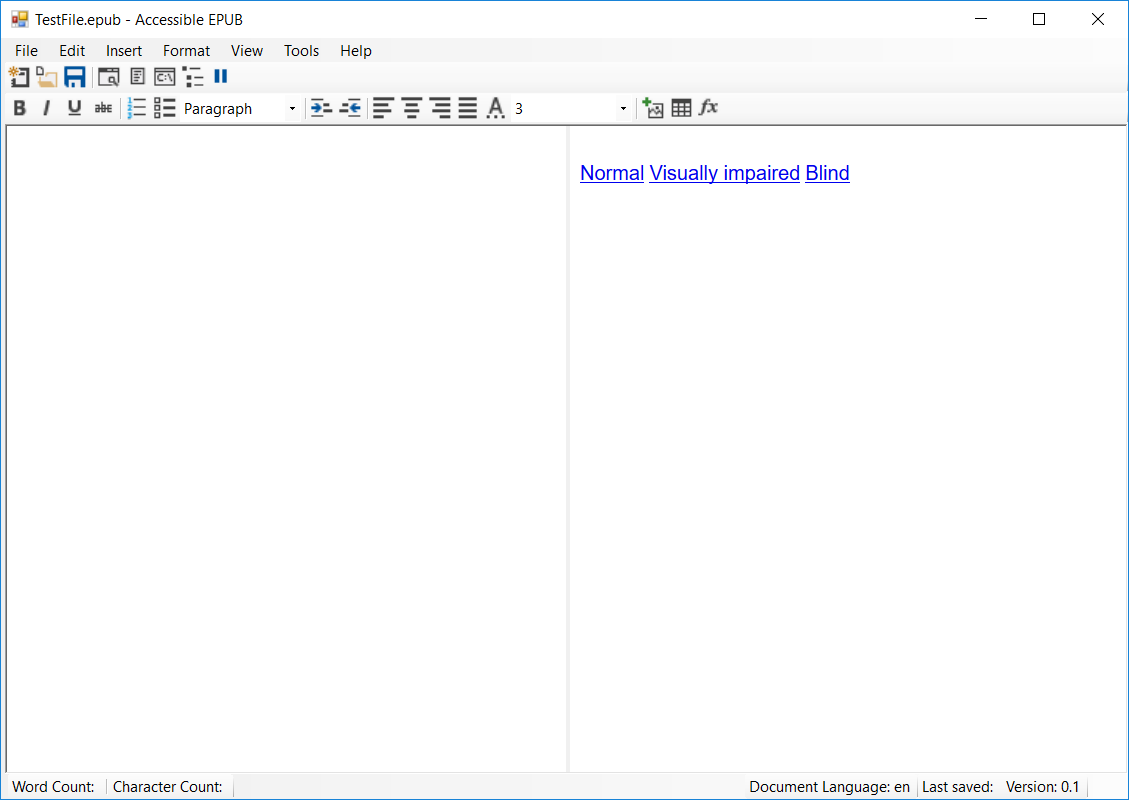
\includegraphics[width=\linewidth]{figures/formCss.png}	
		\caption{Main window with HTML editor and CSS switching preview}
		\label{fig:formCss}
	\end{center}
\end{figure}

\subsubsection{Preview browser}

On the right hand size of the main window is the preview browser. It should display XHTML page in each of three versions(normal, visually impaired, blind). Since the HTML editor uses the WebBrowser control, it would have been easiest to use it on the right side too. However, Internet Explorer is unable to display MathML. Instead of showing the quadratic equation, as shown in figure \ref{fig:quadEquaPng}, it showed figure \ref{fig:IEmathml}. As a result, another browser had to be found. Only two browsers are able properly show MathML, Mozilla Firefox and Safari by Apple. The Firefox engine, Gecko, was chosen as it is open source and had a C\# browser package. After inserting an instance of a \lstinline|GeckoWebBrowser| in the form MathML was displayed properly.

\begin{figure}
	\begin{center}
		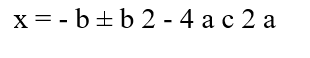
\includegraphics[width=\linewidth/2]{figures/IEmathml.png}	
		\caption{MathML depiction of the quadratic equation in Internet Explorer}
		\label{fig:IEmathml}
	\end{center}
\end{figure}

As seen in figures \ref{fig:formJs} and \ref{fig:formCss}, there is a small difference between the user interface of the JavaScript and CSS versions. The CSS version only uses one browser tab as preview, while the JavaScript version uses three. This is mentioned in chapter \ref{ch:EPUB Document Standard} and is due to the JavaScript version having a separate file named VersionChanger.xhtml, which handles switching versions. In the CSS version the whole content is in one XHTML file. Consequently, the CSS version is very easy to show in the preview. Only the three links shown in figure \ref{fig:css_switch} have to be added to HTML editor content and file is done.

This is much more complicated in the JavaScript version, since the default display style will always be shown. The CSS of the blind and visually impaired version had to be changed. The initial attempt to solve this problem was done by changing the CSS of each browser in a tab and accessing the \lstinline|GeckoStyleSheet| of a browser. Unfortunately, even after changing the \lstinline|GeckoStyleSheet| of a document, it still displayed the default one. An alternative approach consisted of accessing the head(\lstinline|<head>|) of the XHTML document and inserting the CSS there, but this too did not work. These two methods were preferable as they do not have significant input and output (IO) operations. Unfortunately, even slightly altered methods of the two did not function properly. As such an IO intensive approach had to be taken. The XHTML file with the content, \lstinline|Content.XHTML| had to be copied to two new files, \lstinline|BliContent.XHTML| and \lstinline|ImpContent.XHTML| for the blind and visually impaired version, respectively. Then the single line linking the style in XHTML head was replaced with one linking the corresponding CSS. 
Both files are then removed before saving the EPUB and then created again. This is additional overhead, but it was the method which succeeded.

\textcolor{red}{pandoc } %┬▒}

\includegraphics[width=2em]{figures/pandocSigns.png}

%\chapter{Evaluation Editor}
\label{ch:Evaluation Editor}



%%% analyse.tex
%% $Id: analyse.tex 28 2007-01-18 16:31:32Z bless $

\chapter{Analysis}
\label{ch:Analysis}


     % Analyse
%%% entwurf.tex
%% $Id: entwurf.tex 28 2007-01-18 16:31:32Z bless $
%%
%% ==============================
\chapter{Design}
\label{ch:Design}


     % Entwurf
%\chapter{Implementation of your Project}
\label{ch:Implementation}    % Implementierung
%%% eval.tex
%% $Id: eval.tex 5 2005-10-10 20:55:48Z bless $

%%%%%%%%%%%%%
\chapter{Evaluation}
\label{ch:Evaluation}
%%%%%%%%%%%%%
        % Evaluierung
%% zusammenf.tex
%% $Id: zusammenf.tex 4 2005-10-10 20:51:21Z bless $
%%

\chapter{Future Work}
\label{ch:FutureWork}
%% ==============================
%
The Accessible EPUB editor is in a functional state where accessible EPUBs of the both new document standards, CSS and JavaScript can be created and edited. However, there is still much to be done.

The JavaScript document standard supports multiple HTML files as content documents. If the reading system supports local or session storage, it remembers which display style is to be displayed across several HTML files. This is actually the case with JavaScript standard in its current state as the first page with version switching mechanism is on a different page from the actual content. Accessible EPUB does not yet support multiple content pages. One issue mentioned in chapter \ref{ch:AccessibleEPUB Editor} is there are issues with long documents. The preview browser automatically scrolls to the top as soon as the user writes something in the editor. If Accessible EPUB allows the user to add another content page, this problem can be avoided. Furthermore, the user can create documents with several sections and these can be managed individually. This does not work with the CSS standard as CSS changes are local to a HTML file and do not persist across multiple of them.

Future development will focus on usability and simplified import of other document standards. Allowing users to import files of different formats will allow an easier transition to Accessible EPUB. The features will be implemented for two formats at first: text documents and HTML files. Importing text documents is quite simple as the file just has to be read and the contents have to be inserting into the editor. Importing HTML files is a bit more complicated. Instead of inserting into the editor, the back end web browser of the editor must be inserted to. Images and equations will not be in the form of the accessible EPUB document standard, so they have to be converted into the correct form. The program will present the user with a process to examine every image and equation and insert alternative text when necessary. Other formats can be imported with the tool pandoc converting them. It is already a part of Accessible EPUB so it does not require any additional programs.

Another feature advanced users may want is a source code editor. As mentioned in chapter \ref{ch:AccessibleEPUB Editor} a code viewer is already available, but it currently displays the entire file with the inner workings. It is also disabled as there were several issues with it. If a code editor is included, the user should not be able to see the inner workings of the document standard, since editing those might break the EPUB file and make it unreadable. 

\begin{comment}
\begin{figure}
	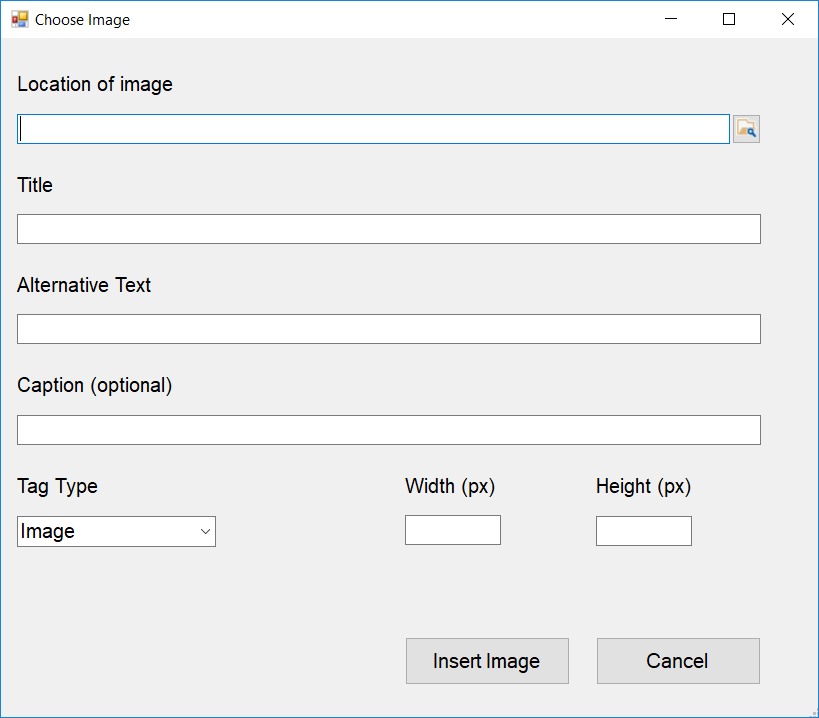
\includegraphics[width=\linewidth]{figures/imageDialogBox.png}	
	\caption{Insert image window of Accessible EPUB}
	\label{fig:imageDialogBox1}
\end{figure}
\end{comment}

To improve accessibility for visually impaired users, it should be possible to add an alternative image which can be a high contrast version of the original image. In addition to the one image document creators have to add, there will be an option to another one. This image will only be shown in the visually impaired display style. If no secondary image was chosen, the regular image will be displayed instead.

Training material has to be prepared so that users can get to know the EPUB standard and Accessible EPUB, like workshops which will users to test the standard and program. There will also be step-by-step tutorials to guide people through the document creation process and how to use all tools in the program.


\begin{comment}
There is still some room for improvement in the compatibility of the EPUB standard, so that it will also be possible to use the documents better with "older" EPUB readers. 
The JavaScript document standard supports multiple HTML files as content documents. If the reader system supports local or session storage, it remembers which version is to be displayed across several HTML files. Accessible EPUB does not yet support this. Adding this feature would allow users to create longer documents and manage individual sections.

Future development will focus on usability and simplified import of other document standards. Currently, users can already import text and HTML documents with certain restrictions so that they can keep their work in these formats. The tool PANDOC can serve as a basis for many formats.
Furthermore, images and formulas will not yet be in the format specified by the document standard during an import, so a wizard will be added that works through each image and formula and allows the user to enter alternative texts.  

Another feature advanced users may want is a source code editor. A code viewer is already available, but currently displays the entire file with the inner workings. The user should not be able to see it, since the processing increases the error possibilities in the document.

We are also considering whether we will start developing suitable readers for various end devices.
\end{comment}

\chapter{Conclusion}
\label{ch:Conclusion}

A short introduction is given where the motivation of this project and a short overview of the file format EPUB is presented. An EPUB document standard has been developed to allow visually impaired, blind and normal-sighted users to use the same document while meeting their respective accessibility requirements. There are two different versions of it, one using JavaScript and the other using CSS. Both versions of the document standard were tested on several reading systems. Only very few of the reading systems were able to show MathML equations and even fewer were able to display the document standards properly. 

EPUB 3 is not widely supported by reading systems. The switching mechanism only worked on four out of fourteen. MathML rendered on nine of them, and many reading systems were chosen because they supported it. Developers still have a lot of work to do for EPUB 3 to have support in their reading systems.

An editor called "Accessible EPUB" was created so that users without programming knowledge can create accessible documents. It allows the user to write text much like in an word processor and insert mathematical equations, images and tables. The document standard uses EPUB 3, which is not yet fully supported by most EPUB reading systems. It is planned to add features to improve the usability of Accessible EPUB, such as importing files of different formats and further tools for accessibility.
  % Future Work
\include{summary}   % Zusammenfassung und Ausblick

%% ++++++++++++++++++++++++++++++++++++++++++
%% Anhang
%% ++++++++++++++++++++++++++++++++++++++++++

\appendix
%\include{anhang_a}
%\include{anhang_b}

%% ++++++++++++++++++++++++++++++++++++++++++
%% Literatur
%% ++++++++++++++++++++++++++++++++++++++++++
%  mit dem Befehl \nocite werden auch nicht 
%  zitierte Referenzen abgedruckt
\cleardoublepage
\phantomsection
\addcontentsline{toc}{chapter}{\bibname}
%%
%\nocite{*} % nur angeben, wenn auch nicht im Text zitierte Quellen 
           % erscheinen sollen
%\bibliographystyle{itmabbrv} % mit abgekürzten Vornamen der Autoren
%\bibliographystyle{gerplain} % abbrvnat unsrtnat
% spezielle Zitierstile: Labels mit vier Buchstaben und Jahreszahl
%\bibliographystyle{itmalpha}  % ausgeschriebene Vornamen der Autoren

\sloppy
\printbibliography
%% ++++++++++++++++++++++++++++++++++++++++++
%% Index
%% ++++++++++++++++++++++++++++++++++++++++++
\ifnotdraft{
\cleardoublepage
\phantomsection
\printindex            % Index, Stichwortverzeichnis
}

\end{document}
%% end of file

